 \documentclass[oneside,11pt]{article}


\usepackage{soul}
\usepackage{natbib}
\usepackage{hyperref}
\usepackage{bookmark}
\usepackage{graphicx}             
\graphicspath{{./Figuras/}}
\usepackage[dvipsnames]{xcolor}
\usepackage{todonotes}
\usepackage{makecell}
\usepackage[margin=1in]{geometry}
\usepackage{float}                
\usepackage{amsmath}
\usepackage{amscd}
\usepackage{amsfonts}
\usepackage{amssymb}
\usepackage{bbm}
\usepackage{booktabs}
\usepackage{nameref}
\usepackage{multirow}
\usepackage[nokeyprefix]{refstyle}
\usepackage{rotating}
\usepackage{threeparttable}
\usepackage{afterpage}
\usepackage{lscape}
\usepackage{enumerate}
\usepackage{caption}
\usepackage{subcaption}
\usepackage{epstopdf}
\usepackage{setspace}
\usepackage{svg}
\usepackage{dsfont}
\usepackage{amsthm}
\usepackage{tocloft}
\usepackage{etoc}
\usepackage{lmodern}
\usepackage{bm}
\usepackage[T1]{fontenc}
\usepackage{tgpagella}

\epstopdfDeclareGraphicsRule{.tiff}{png}{.png}{convert #1 \OutputFile}
\AppendGraphicsExtensions{.tiff}

\epstopdfDeclareGraphicsRule{.tif}{png}{.png}{convert #1 \OutputFile}
\AppendGraphicsExtensions{.tif}

\def\sym#1{\ifmmode^{#1}\else\(^{#1}\)\fi}

\usepackage{tikz}
\usetikzlibrary{shapes.geometric, arrows}
\usetikzlibrary{calc}
\usetikzlibrary{matrix}

\tikzset{ 
    table/.style={
        matrix of nodes,
        row sep=-\pgflinewidth,
        column sep=-\pgflinewidth,
        nodes={
            rectangle,
            draw=black,
            align=center
        },
        minimum height=1.5em,
        text depth=0.5ex,
        text height=2ex,
        nodes in empty cells,
%%
        every even row/.style={
            nodes={fill=gray!20}
        },
        column 1/.style={
            nodes={text width=2em,font=\bfseries}
        },
        row 1/.style={
            nodes={
                fill=black,
                text=white,
                font=\bfseries
            }
        }
    }
}


\usepackage{colortbl}
\usepackage{url}
\urlstyle{rm}
\definecolor{darkblue}{rgb}{0,0,.4}
\hypersetup{colorlinks=true, breaklinks=true, citecolor=Maroon, linkcolor=darkblue, menucolor=darkblue, urlcolor=darkblue}

\newtheorem{theorem}{Theorem}
\newtheorem{claim}[theorem]{Claim}
\newtheorem{prop}[theorem]{Proposition} 
\newtheorem{cor}[theorem]{Corollary} 
\newtheorem{assumption}{Assumption} 
\newtheorem{lem}{Lemma} 

\DeclareRobustCommand{\hlgr}[1]{{\sethlcolor{green}\hl{#1}}}


\usepackage{comment}
%para esconder columnas en tablas (enrique)
\usepackage{array}
\newcolumntype{H}{>{\setbox0=\hbox\bgroup}c<{\egroup}@{}}
\linespread{1.25}

\newcommand{\wh}{\widehat}
\usepackage{anyfontsize}

\usepackage[linesnumbered,vlined,ruled,commentsnumbered]{algorithm2e}

\DontPrintSemicolon
\newcommand{\To}{\mbox{\upshape\bfseries to}}
\newcommand{\E}{\mathbb{E}}

\DeclareCaptionFormat{cont}{#1 (cont.)#2#3\par}
%%% HELPER CODE FOR DEALING WITH EXTERNAL REFERENCES
\usepackage{xr}
\makeatletter
\newcommand*{\addFileDependency}[1]{
  \typeout{(#1)}
  \@addtofilelist{#1}
  \IfFileExists{#1}{}{\typeout{No file #1.}}
}
\makeatother


\newcommand*{\myexternaldocument}[1]{
    \externaldocument{#1}
    \addFileDependency{#1.tex}
    \addFileDependency{#1.aux}
}

%\myexternaldocument{OA}

%%%%%%%%%%%%%%%%%%%%%%%%%%%%%%%% DOCUMENT
\begin{document}


\title{IMSS RPCI \thanks{We want to thank.}}
\author{Eduardo Alcaraz \and Gabriela López \and Luis Martínez \and Marco Medina \and Enrique Seira  \thanks{Seira: ITAM, enrique.seira@gmail.com (corresponding author); Alcaraz: IMSS, eduardo.alcarazp@imss.gob.mx; López: IMSS, ; Martínez: IMSS, luis.martinezch@imss.gob.mx; Medina:  ITAM, marco.medina@itam.mx}}
\date{This draft:  \today \\[2 cm]}

%\vspace{.5in}


\maketitle
\thispagestyle{empty}
\begin{abstract}

%Abstract here. 

\end{abstract}

\vspace{.3in}

\textbf{Keywords: }

\textbf{JEL codes:}

\newpage

\pagenumbering{arabic}
\etocdepthtag.toc{mtchapter}
\etocsettagdepth{mtchapter}{subsection}
\etocsettagdepth{mtappendix}{none}



\section{Introduction}
Workers in Mexico with formal jobs are registered by their employer to the Instituto Mexicano del Seguro Social (IMSS), the
Mexican social security agency. Employers report to IMSS the wage earned by the worker. Taxes and employer's social security contributions are proportional to the reported wage. Employers may under report the actual wage earned by the worker \citep{kumler2020enlisting}. Under reporting wages can be perjudicial to the worker, since social security, retirement and pension benefits depend on the reported wage. Workers tend to discover under reporting until they are about to retire, when they ask for their report on quoted weeks (quoted weeks are the period of time quoted by the worker with the IMSS). The report contains the information for each job the worker has been registered for at IMSS, including wages, employers firm name, and tenure. Since they ask for the report when they are about to retire, there isn't much they can do if they find under reporting. With this in mind, IMSS created the RPCI, a personalized report on the worker's current job. The objective is to make access to information on the worker's register easier.

\section{Context} \label{context}

\section{Experimental Design} \label{Experiment}

\subsection{Survey Data and Summary Statistics}

\subsection{Balance in the Experimental Sample}

\section{Experimental Analysis} \label{experiment}

\subsection{Matching} \label{matching}
We perform matching using nearest neighbor matching with replacement and bias-adjustment, procedure developed by \cite{abadie2006large} as described by \cite{imbens2015matching}. We match using worker characteristics at baseline such as gender, age range, their mean wage and the wage standard deviation during 2020, temporary status, outsourcing status, and characteristics of the firm at their baseline job, such as if their job was in a government agency, firm size, firm industry and state. 

We calculate the distance between two values of the covariate vector $x$ and $x'$, using the Mahalonobis distance metric and the sample covariance matrix of covariates as weighting matrix: $\lVert x,x' \rVert = (x-x')'\hat{\Omega}^{-1}_{X}(x-x')$. Now for each worker $i = 1, \dots, N$ in the sample, let $\ell(i)$ be the index for the closest match, defined as:

$$\ell(i) = \arg \min_{j:W_j \neq W_i} = \rVert X_i - X_j \lVert$$ 

where we take the first match in case of ties (we set a seed and randomize the order of the observations before matching to get a stable match). Given $\ell(i)$ define:

$$\hat{Y}_i(0) = 
\begin{cases}
Y_{i}^{obs} &\quad \text{if } W_i = 0\\ 
Y_{\ell(i)} &\quad \text{if } W_i = 1
\end{cases}
\quad \quad
\hat{Y}_i(1) = 
\begin{cases}
Y_{\ell(i)} &\quad \text{if } W_i = 0\\ 
Y_{i}^{obs} &\quad \text{if } W_i = 1
\end{cases}$$

Define the matched values for the covariates:

$$\hat{X}_i(0) = 
\begin{cases}
X_{i} &\quad \text{if } W_i = 0\\ 
X_{\ell(i)} &\quad \text{if } W_i = 1
\end{cases}
\quad \quad
\hat{X}_i(1) = 
\begin{cases}
X_{\ell(i)} &\quad \text{if } W_i = 0\\ 
X_{i} &\quad \text{if } W_i = 1
\end{cases}$$

This leads to a matched sample with $N$ pairs.

\section{Conclusion} \label{conclusion}


%%%%%%%%%%%%%%%%%%%%%%%%%%%%%%%%%%%%%%%%%%%%%%%%%%%%%%%%%%%%%

\newpage

%%%%%%%%%%%%%%%%%%%%%%%%%%%%%%%%%%%%%%%%%%%%%%%%%%%%%%%%%%%%%
%BIBLIOGRAPHY


\clearpage
\bibliographystyle{authordate1}
%\bibliographystyle{amsalpha}
%\bibliographystyle{AEA}

\bibliography{References}



%\FloatBarrier
%%%%%%%%%%%%%%%%%%%%%%%%%%%%%%%%%%%%%%%%

\clearpage
\singlespacing

\section{Tables}

\begin{table}[H]
    \caption{Balance table}
    \label{balance_1}
    \begin{center}
    \scriptsize{% Table generated by Excel2LaTeX from sheet 'SelfUpdate_balance_1'
\begin{tabular}{r|rrr}
\toprule
\toprule
\multicolumn{1}{p{12.085em}|}{} & \multicolumn{1}{c}{Worker didn't} & \multicolumn{1}{c}{Worker} &  \\
\multicolumn{1}{p{12.085em}|}{Variables} & \multicolumn{1}{c}{Downloaded RPCI} & \multicolumn{1}{c}{Downloaded RPCI} & \multicolumn{1}{c}{t-test} \\
\midrule
\multicolumn{1}{p{12.085em}|}{} &                 &                 &  \\
\multicolumn{1}{p{12.085em}|}{Women} & \multicolumn{1}{c}{0.394} & \multicolumn{1}{c}{0.404} & \multicolumn{1}{c}{0.010*} \\
\multicolumn{1}{p{12.085em}|}{} & \multicolumn{1}{c}{(0.489)} & \multicolumn{1}{c}{(0.491)} & \multicolumn{1}{c}{(0.005)} \\
\multicolumn{1}{p{12.085em}|}{Wage} & \multicolumn{1}{c}{365.076} & \multicolumn{1}{c}{387.122} & \multicolumn{1}{c}{22.046***} \\
                & \multicolumn{1}{c}{(375.164)} & \multicolumn{1}{c}{(379.881)} & \multicolumn{1}{c}{(4.496)} \\
\multicolumn{1}{p{12.085em}|}{Temporary worker} & \multicolumn{1}{c}{0.169} & \multicolumn{1}{c}{0.150} & \multicolumn{1}{c}{-0.019***} \\
\multicolumn{1}{p{12.085em}|}{} & \multicolumn{1}{c}{(0.375)} & \multicolumn{1}{c}{(0.357)} & \multicolumn{1}{c}{(0.004)} \\
\multicolumn{1}{p{12.085em}|}{Government} & \multicolumn{1}{c}{0.066} & \multicolumn{1}{c}{0.079} & \multicolumn{1}{c}{0.013***} \\
\multicolumn{1}{p{12.085em}|}{} & \multicolumn{1}{c}{(0.249)} & \multicolumn{1}{c}{(0.270)} & \multicolumn{1}{c}{(0.003)} \\
\multicolumn{1}{p{12.085em}|}{Outsourcing} & \multicolumn{1}{c}{0.251} & \multicolumn{1}{c}{0.292} & \multicolumn{1}{c}{0.041***} \\
                & \multicolumn{1}{c}{(0.434)} & \multicolumn{1}{c}{(0.455)} & \multicolumn{1}{c}{(0.005)} \\
\multicolumn{1}{p{12.085em}|}{Agriculture} & \multicolumn{1}{c}{0.048} & \multicolumn{1}{c}{0.013} & \multicolumn{1}{c}{-0.036***} \\
\multicolumn{1}{p{12.085em}|}{} & \multicolumn{1}{c}{(0.214)} & \multicolumn{1}{c}{(0.111)} & \multicolumn{1}{c}{(0.003)} \\
\multicolumn{1}{p{12.085em}|}{Extractive Ind.} & \multicolumn{1}{c}{0.006} & \multicolumn{1}{c}{0.006} & \multicolumn{1}{c}{-0.000} \\
\multicolumn{1}{p{12.085em}|}{} & \multicolumn{1}{c}{(0.077)} & \multicolumn{1}{c}{(0.076)} & \multicolumn{1}{c}{(0.001)} \\
\multicolumn{1}{p{12.085em}|}{Transformation Ind.} & \multicolumn{1}{c}{0.261} & \multicolumn{1}{c}{0.204} & \multicolumn{1}{c}{-0.057***} \\
\multicolumn{1}{p{12.085em}|}{} & \multicolumn{1}{c}{(0.439)} & \multicolumn{1}{c}{(0.403)} & \multicolumn{1}{c}{(0.005)} \\
\multicolumn{1}{p{12.085em}|}{Construction Ind.} & \multicolumn{1}{c}{0.099} & \multicolumn{1}{c}{0.081} & \multicolumn{1}{c}{-0.018***} \\
\multicolumn{1}{p{12.085em}|}{} & \multicolumn{1}{c}{(0.299)} & \multicolumn{1}{c}{(0.273)} & \multicolumn{1}{c}{(0.004)} \\
\multicolumn{1}{p{12.085em}|}{Electric Ind.} & \multicolumn{1}{c}{0.006} & \multicolumn{1}{c}{0.007} & \multicolumn{1}{c}{0.000} \\
\multicolumn{1}{p{12.085em}|}{} & \multicolumn{1}{c}{(0.078)} & \multicolumn{1}{c}{(0.081)} & \multicolumn{1}{c}{(0.001)} \\
\multicolumn{1}{p{12.085em}|}{Commerce} & \multicolumn{1}{c}{0.196} & \multicolumn{1}{c}{0.227} & \multicolumn{1}{c}{0.031***} \\
                & \multicolumn{1}{c}{(0.397)} & \multicolumn{1}{c}{(0.419)} & \multicolumn{1}{c}{(0.005)} \\
\multicolumn{1}{p{12.085em}|}{Transport} & \multicolumn{1}{c}{0.056} & \multicolumn{1}{c}{0.062} & \multicolumn{1}{c}{0.006**} \\
\multicolumn{1}{p{12.085em}|}{} & \multicolumn{1}{c}{(0.229)} & \multicolumn{1}{c}{(0.240)} & \multicolumn{1}{c}{(0.003)} \\
\multicolumn{1}{p{12.085em}|}{Personal services} & \multicolumn{1}{c}{0.232} & \multicolumn{1}{c}{0.293} & \multicolumn{1}{c}{0.061***} \\
\multicolumn{1}{p{12.085em}|}{} & \multicolumn{1}{c}{(0.422)} & \multicolumn{1}{c}{(0.455)} & \multicolumn{1}{c}{(0.005)} \\
\multicolumn{1}{p{12.085em}|}{Social services} & \multicolumn{1}{c}{0.095} & \multicolumn{1}{c}{0.109} & \multicolumn{1}{c}{0.013***} \\
\multicolumn{1}{p{12.085em}|}{} & \multicolumn{1}{c}{(0.294)} & \multicolumn{1}{c}{(0.311)} & \multicolumn{1}{c}{(0.004)} \\
\midrule
\multicolumn{1}{p{12.085em}|}{Observations} & \multicolumn{1}{c}{316,807} & \multicolumn{1}{c}{8,585} & \multicolumn{1}{c}{325,392} \\
                &                 &                 &  \\
\bottomrule
\bottomrule
\end{tabular}%
}
    %\textit{Do file: balance_rpci.do}
    \end{center}
\end{table}

\scriptsize{
\noindent \textit{Sample:} 1\% of the workers registered at the Mexican Institute of Social Security (IMSS) between January 2020 and August 2022. Balance table elaborated with the workers' characteristics during 2020, before the launch of the RPCI app.
}

\clearpage

\subsection{TWFE}

\begin{table}[H]
    \caption{RPCI effect on wage}
    \label{twfe_wage}
    \begin{center}
    \scriptsize{% Table generated by Excel2LaTeX from sheet 'twfe_wage'
\begin{tabular}{ccccccc}
\toprule
\toprule
      & (1)   & (2)   & (3)   & (4)   & (5)   & (6) \\
\cmidrule{2-7}      & \multicolumn{6}{c}{\textit{A) Wage}} \\
\midrule
RPCI  & 9.8*** & 6.5*** & 8.8*** & 8.4*** & 9.4*** & 4.3** \\
      & (2.04) & (2.12) & (2.12) & (2.12) & (2.11) & (2.09) \\
Constant & 436.9*** & 448.7*** & 448.6*** & 448.6*** & 448.6*** & 448.7*** \\
      & (0.02) & (0.02) & (0.02) & (0.02) & (0.02) & (0.02) \\
Mean  & 437.0 & 448.7 & 448.7 & 448.7 & 448.8 & 448.8 \\
\cmidrule{2-7}      & \multicolumn{6}{c}{\textit{B) Log Wage}} \\
\midrule
RPCI  & 0.02*** & 0.01*** & 0.02*** & 0.02*** & 0.02*** & 0.01*** \\
      & (0.004) & (0.004) & (0.004) & (0.004) & 0.004 & 0.004 \\
Constant & 5.78*** & 5.80*** & 5.80*** & 5.80*** & 5.80*** & 5.80*** \\
      & (0.000) & (0.000) & (0.000) & (0.000) & (0.000) & (0.000) \\
Mean  & 5.78  & 5.80  & 5.80  & 5.80  & 5.80  & 5.80 \\
\midrule
Observations & 6,380,963 & 5,913,975 & 5,913,975 & 5,913,975 & 5,913,144 & 5,913,144 \\
Workers & 306,909 & 248,935 & 248,935 & 248,935 & 248,830 & 248,830 \\
Firms & 164,727 & 145,687 & 145,687 & 145,687 & 145,648 & 145,648 \\
\midrule
\textit{Linear Trends FE} &       &       &       &       &       &  \\
Age   &       & \checkmark &       &       &       & \checkmark \\
Firm Industry &       &       & \checkmark &       &       & \checkmark \\
State &       &       &       & \checkmark &       & \checkmark \\
Wage Decile &       &       &       &       & \checkmark & \checkmark \\
\bottomrule
\bottomrule
\end{tabular}%
}
    %\textit{Do file: twfe_rpci.do}
    \end{center}
\end{table}

\scriptsize{
\noindent This table shows the effect of registering to the RPCI on the reported wage. \textit{Sample:} 1\% of the workers registered at the Mexican Institute of Social Security (IMSS) between January 2020 and August 2022. Regressions use the TWFE specification $y_{it} = \gamma_{i} + \theta_{t}+ \beta RPCI_{it} +\epsilon_{it}$, where $\gamma_{i}$ are dummies for each worker id, $\theta_{t}$ are dummies for each monthly period, and $RPCI_{it}$ are dummies where 1 means that the worker registered for the RPCI during that month or previous month. Regressions on columns (2)-(6) include fixed effects on linear trends, by interacting dummies on worker's baseline characteristics with a set of dummies for each quarterly period: (2) age group, (3) firm industry, (4) state, (5) wage decile, (6) all previous. Robust standard errors clustered by worker id in parenthesis. *** $p<0.01$, ** $p<0.05$, * $p<0.1$.
}

\clearpage

\begin{table}[H]
    \caption{RPCI effect on wage for workers with a unique employer}
    \label{twfe_wage_same_idrfc}
    \begin{center}
    \scriptsize{% Table generated by Excel2LaTeX from sheet 'twfe_wage_same_idrfc'
\begin{tabular}{c|cccc|cccc}
\toprule
\toprule
      & \multicolumn{4}{c|}{Wage}     & \multicolumn{4}{c}{Log Wage} \\
Variables & (1a)  & (1b)  & (1c)  & (1d)  & (2a)  & (2b)  & (2c)  & (2d) \\
\midrule
      &       &       &       &       &       &       &       &  \\
RPCI  & 9.2*** & 8.8*** & 5.9** & 6.3*** & 0.00  & 0.01* & 0.01*** & 0.01*** \\
      & (2.30) & (2.29) & (2.33) & (2.33) & (0.004) & (0.003) & (0.003) & (0.003) \\
Constant & 466.4*** & 466.4*** & 482.7*** & 482.7*** & 5.83*** & 5.83*** & 5.86*** & 5.86*** \\
      & (0.02) & (0.02) & (0.02) & (0.02) & (0.000) & (0.000) & (0.000) & (0.000) \\
      &       &       &       &       &       &       &       &  \\
\midrule
Observations & 3,265,260 & 3,265,260 & 2,983,149 & 2,983,149 & 3,265,260 & 3,265,260 & 2,983,149 & 2,983,149 \\
Mean  & 466.5 & 466.5 & 482.7 & 482.7 & 5.83  & 5.83  & 5.86  & 5.86 \\
Workers & 161,085 & 161,085 & 122,937 & 122,937 & 161,085 & 161,085 & 122,937 & 122,937 \\
Firms & 77,067 & 77,067 & 58,909 & 58,909 & 77,067 & 77,067 & 58,909 & 58,909 \\
\bottomrule
\bottomrule
\end{tabular}%
}
    %\textit{Do file: twfe_rpci.do}
    \end{center}
\end{table}

\scriptsize{
\noindent \textit{Sample:} 1\% of the workers registered at the Mexican Institute of Social Security (IMSS) between January 2020 and August 2022, restricted to those workers with a unique employer across the 33 months of the sample. Regressions on columns (a) use the TWFE specification $y_{it} = \gamma_{i} + \theta_{t}+ \beta RPCI_{it} +\epsilon_{it}$, where $\gamma_{i}$ are dummies for each worker id, $\theta_{t}$ are dummies for each monthly period, and $RPCI_{it}$ are dummies where 1 means that the worker registered for the RPCI during that month or previous month. Regressions on columns (b) include dummies for each state interacted with a set of dummies for each quarterly period. Regressions on columns (c) include dummies for each wage decile of the wage distribution during 2020, interacted with a set of dummies for each quarterly period. Regressions on columns (d) include dummies for each state and dummies for each wage decile of the wage distribution during 2020, both interacted with dummies for each quarterly period. Robust standard errors clustered by worker id in parenthesis. *** $p<0.01$, ** $p<0.05$, * $p<0.1$.
\todo[inline]{Marco: update this table with the same format as \ref{twfe_wage}}
}


\clearpage

\begin{table}[H]
    \caption{RPCI effect on discharges and job changes}
    \label{twfe_job}
    \begin{center}
    \scriptsize{% Table generated by Excel2LaTeX from sheet 'twfe_job'
\begin{tabular}{c|cccccc}
\toprule
\toprule
      & Enrolled & Enrollment & Discharge & Perm. Discharge & Wage Change & Job Change \\
Variables & \multicolumn{1}{p{7.085em}}{(1)} & \multicolumn{1}{p{7.085em}}{(2)} & \multicolumn{1}{p{7.085em}}{(3)} & \multicolumn{1}{p{7.085em}}{(4)} & \multicolumn{1}{p{7.085em}}{(5)} & \multicolumn{1}{p{7.085em}}{(6)} \\
\midrule
      &       &       &       &       &       &  \\
RPCI  & \multicolumn{1}{p{7.085em}}{0.050***} & 0.001 & \multicolumn{1}{p{7.085em}}{0.011***} & \multicolumn{1}{p{7.085em}}{0.010***} & 0.002 & \multicolumn{1}{p{7.085em}}{0.004***} \\
      & (0.004) & (0.001) & (0.001) & (0.000) & (0.002) & (0.001) \\
Constant & \multicolumn{1}{p{7.085em}}{0.725***} & \multicolumn{1}{p{7.085em}}{0.025***} & \multicolumn{1}{p{7.085em}}{0.029***} & \multicolumn{1}{p{7.085em}}{0.010***} & \multicolumn{1}{p{7.085em}}{0.327***} & \multicolumn{1}{p{7.085em}}{0.025***} \\
      & (0.000) & (0.000) & (0.000) & (0.000) & (0.000) & (0.000) \\
      &       &       &       &       &       &  \\
\midrule
Observations & 8,164,128 & 8,164,128 & 8,164,128 & 8,164,128 & 5,645,627 & 5,645,627 \\
Mean  & 0.725 & 0.025 & 0.029 & 0.010 & 0.327 & 0.025 \\
Workers & 255,129 & 255,129 & 255,129 & 255,129 & 242,602 & 242,602 \\
Firms & 147,147 & 147,147 & 147,147 & 147,147 & 137,124 & 137,124 \\
\bottomrule
\bottomrule
\end{tabular}%
}
    %\textit{Do file: twfe_rpci.do}
    \end{center}
\end{table}

\scriptsize{
\noindent \textit{Sample:} 1\% of the workers registered at the Mexican Institute of Social Security (IMSS) between January 2020 and August 2022. \textit{Discharge} is a dummy where 1 means the worker had a job registered during period $t$, but didn't have one during period $t+1$. \textit{Permanent Discharge} is a dummy where 1 means the worker had a register during period $t$, but never had a job registered again for the rest of the months in the sample. \textit{Job Change} is a dummy where 1 means the worker had a job registered during period $t$, and has a job registered at a different firm during period $t+1$. Regressions use the TWFE specification $y_{it} = \gamma_{i} + \theta_{t}+ \beta RPCI_{it} +\epsilon_{it}$, where $\gamma_{i}$ are dummies for each worker id, $\theta_{t}$ are dummies for each monthly period, and $RPCI_{it}$ are dummies where 1 means that the worker registered for the RPCI during that month or previous month. Regressions include fixed effects on linear trends for age group, firm industry, state and wage decile, by interacting dummies on worker's baseline characteristics with a set of dummies for each quarterly period. Robust standard errors clustered by worker id in parenthesis. *** $p<0.01$, ** $p<0.05$, * $p<0.1$.
}

\clearpage

\begin{table}[H]
    \caption{RPCI effect on job changes according to wage changes}
    \label{twfe_job_change_wage}
    \begin{center}
    \scriptsize{% Table generated by Excel2LaTeX from sheet 'twfe_job_change_wage'
\begin{tabular}{c|ccc}
\toprule
\toprule
      & Job Change & Job Change & Job Change \\
      & Higher Wage & Lower Wage & Same Wage \\
Variables & (1)   & (2)   & (3) \\
\midrule
      &       &       &  \\
RPCI  & 0.000 & 0.001 & 0.000 \\
      & (0.001) & (0.001) & (0.000) \\
Constant & \multicolumn{1}{p{6.25em}}{0.011***} & \multicolumn{1}{p{6.25em}}{0.009***} & \multicolumn{1}{p{6.25em}}{0.004***} \\
      & (0.000) & (0.000) & (0.000) \\
      &       &       &  \\
\midrule
Observations & 5,915,501 & 5,915,501 & 5,915,501 \\
Mean  & 0.011 & 0.009 & 0.004 \\
Workers & 248,846 & 248,846 & 248,846 \\
Firms & 145,687 & 145,687 & 145,687 \\
\bottomrule
\bottomrule
\end{tabular}%
}
    %\textit{Do file: twfe_rpci.do}
    \end{center}
\end{table}

\scriptsize{
\noindent \textit{Sample:} 1\% of the workers registered at the Mexican Institute of Social Security (IMSS) between January 2020 and August 2022. \textit{Job Change Higher Wage}, \textit{Job Change Lower Wage}, and \textit{Job Change Same Wage} are a dummies where 1 means the worker had a job registered during period $t$, and has a job registered at a different firm during period $t+1$, and their new wage is higher, lower or the same as in the former job. Regressions use the TWFE specification $y_{it} = \gamma_{i} + \theta_{t}+ \beta RPCI_{it} +\epsilon_{it}$, where $\gamma_{i}$ are dummies for each worker id, $\theta_{t}$ are dummies for each monthly period, and $RPCI_{it}$ are dummies where 1 means that the worker registered for the RPCI during that month or previous month. Regressions include fixed effects on linear trends for age group, firm industry, state and wage decile, by interacting dummies on worker's baseline characteristics with a set of dummies for each quarterly period. Robust standard errors clustered by worker id in parenthesis. *** $p<0.01$, ** $p<0.05$, * $p<0.1$.
\todo[inline]{Marco: I have to create a similar table, but for Discharge instead of Job Change. Q: how to define higher / lower / same wage if you were discharged and we won't observe your wage for the next period?}
}

\clearpage

\subsection{TWFE - Heterogeneity}

\begin{table}[H]
    \caption{RPCI effect on wage by worker characteristics}
    \label{twfe_wage_hetero_wrk_char}
    \begin{center}
    \scriptsize{% Table generated by Excel2LaTeX from sheet 'twfe_wage_hetero_wrk_char'
\begin{tabular}{ccccc}
\toprule
\toprule
      & Men   & Women & Outsourcing & Temporary \\
      & (1)   & (2)   & (3)   & (4) \\
\cmidrule{2-5}      & \multicolumn{4}{c}{\textit{A) Wage}} \\
\midrule
RPCI  & 9.3*** & -2.8  & -1.7  & 10.5** \\
      & (2.960) & (2.720) & (4.230) & (5.260) \\
Constant & 470.7*** & 413.5*** & 521.5*** & 395.6*** \\
      & (0.030) & (0.030) & (0.060) & (0.060) \\
Mean  & 470.8 & 413.5 & 521.5 & 395.7 \\
\cmidrule{2-5}      & \multicolumn{4}{c}{\textit{B) Log Wage}} \\
\midrule
RPCI  & 0.02*** & 0.00  & 0.00  & 0.03** \\
      & (0.005) & (0.005) & (0.007) & (0.010) \\
Constant & 5.83*** & 5.74*** & 5.95*** & 5.73*** \\
      & (0.000) & (0.000) & (0.000) & (0.000) \\
Mean  & 5.83  & 5.74  & 5.95  & 5.73 \\
\midrule
Observations & 3,636,851 & 2,276,293 & 1,529,005 & 834,197 \\
Workers & 153,534 & 95,296 & 63,303 & 41,351 \\
Firms & 109,939 & 64,446 & 36,040 & 36,671 \\
\bottomrule
\bottomrule
\end{tabular}%
}
    %\textit{Do file: twfe_rpci.do}
    \end{center}
\end{table}
\scriptsize{
\noindent This table looks into heterogeneity in the RPCI effect by worker characteristics. Each column conditions on a worker characteristics at baseline, during 2020, previous to the RPCI launch. Columns (1) and (2) condition on the worker gender. Column (3) conditions on workers hired through outsourcing. Column (4) conditions on temporary workers. \textit{Sample:} 1\% of the workers registered at the Mexican Institute of Social Security (IMSS) between January 2020 and August 2022. Regressions use the TWFE specification $y_{it} = \gamma_{i} + \theta_{t}+ \beta RPCI_{it} +\epsilon_{it}$, where $\gamma_{i}$ are dummies for each worker id, $\theta_{t}$ are dummies for each monthly period, and $RPCI_{it}$ are dummies where 1 means that the worker registered for the RPCI during that month or previous month. Regressions include fixed effects on linear trends for age group, firm industry, state and wage decile, by interacting dummies on worker's baseline characteristics with a set of dummies for each quarterly period. Robust standard errors clustered by worker id in parenthesis. *** $p<0.01$, ** $p<0.05$, * $p<0.1$.
\textit{Do file: twfe\_heterogeneity\_rpci.do}
}

\clearpage

\begin{table}[H]
    \caption{RPCI effect on discharge and job change by worker characteristics}
    \label{twfe_job_hetero_wrk_char}
    \begin{center}
    \scriptsize{% Table generated by Excel2LaTeX from sheet 'twfe_job_hetero_wrk_char'
\begin{tabular}{ccccc}
\toprule
\toprule
      & Men   & Women & Outsourcing & Temporary \\
      & (1)   & (2)   & (3)   & (4) \\
\cmidrule{2-5}      & \multicolumn{4}{c}{\textit{A) Discharge}} \\
\midrule
RPCI  & -0.002 & 0.002 & 0.004 & -0.001 \\
      & (0.002) & (0.002) & (0.002) & (0.003) \\
Constant & 0.041*** & 0.034*** & 0.038*** & 0.071*** \\
      & (0.000) & (0.000) & (0.000) & (0.000) \\
Mean  & 0.04  & 0.03  & 0.04  & 0.07 \\
\cmidrule{2-5}      & \multicolumn{4}{c}{\textit{B) Permanent Discharge}} \\
\midrule
RPCI  & -0.001 & 0.003*** & 0.002* & -0.004** \\
      & (0.001) & (0.001) & (0.001) & (0.002) \\
Constant & 0.013*** & 0.013*** & 0.012*** & 0.021*** \\
      & (0.000) & (0.000) & (0.000) & (0.000) \\
Mean  & 0.01  & 0.01  & 0.01  & 0.02 \\
\cmidrule{2-5}      & \multicolumn{4}{c}{\textit{C) Job Change}} \\
\midrule
RPCI  & 0.001 & 0.000 & 0.004** & 0.000 \\
      & (0.001) & (0.001) & (0.002) & (0.003) \\
Constant & 0.026*** & 0.020*** & 0.038*** & 0.033*** \\
      & (0.000) & (0.000) & (0.000) & (0.000) \\
Mean  & 0.03  & 0.02  & 0.04  & 0.03 \\
\midrule
Observations & 3,638,670 & 2,276,831 & 1,529,153 & 834,668 \\
Workers & 153,547 & 95,299 & 63,304 & 41,353 \\
Firms & 109,958 & 64,469 & 36,045 & 36,678 \\
\bottomrule
\bottomrule
\end{tabular}%
}
    %\textit{Do file: twfe_rpci.do}
    \end{center}
\end{table}
\scriptsize{
\noindent This table looks into heterogeneity in the RPCI effect by worker characteristics. Each column conditions on a worker characteristics at baseline, during 2020, previous to the RPCI launch. Columns (1) and (2) condition on the worker gender. Column (3) conditions on workers hired through outsourcing. Column (4) conditions on temporary workers. \textit{Sample:} 1\% of the workers registered at the Mexican Institute of Social Security (IMSS) between January 2020 and August 2022. \textit{Discharge} is a dummy where 1 means the worker had a job registered during period $t$, but didn't have one during period $t+1$. \textit{Permanent Discharge} is a dummy where 1 means the worker had a register during period $t$, but never had a job registered again for the rest of the months in the sample. \textit{Job Change} is a dummy where 1 means the worker had a job registered during period $t$, and has a job registered at a different firm during period $t+1$. Regressions use the TWFE specification $y_{it} = \gamma_{i} + \theta_{t}+ \beta RPCI_{it} +\epsilon_{it}$, where $\gamma_{i}$ are dummies for each worker id, $\theta_{t}$ are dummies for each monthly period, and $RPCI_{it}$ are dummies where 1 means that the worker registered for the RPCI during that month or previous month. Regressions include fixed effects on linear trends for age group, firm industry, state and wage decile, by interacting dummies on worker's baseline characteristics with a set of dummies for each quarterly period. Robust standard errors clustered by worker id in parenthesis. *** $p<0.01$, ** $p<0.05$, * $p<0.1$.
\textit{Do file: twfe\_heterogeneity\_rpci.do}
}

\clearpage

\begin{landscape}

\begin{table}[H]
    \caption{RPCI effect on wage by firm characteristics}
    \label{twfe_wage_hetero_firm_char}
    \begin{center}
    \scriptsize{% Table generated by Excel2LaTeX from sheet 'twfe_wage_hetero_firm_char'
\begin{tabular}{ccccccccc}
\toprule
\toprule
      & Transf. Ind. & Constr. Ind. & Commerce & Transport & Pers. Serv. & Soc. Serv. & Small Firm & Big Firm \\
      & (1)   & (2)   & (3)   & (4)   & (5)   & (6)   & (7)   & (8) \\
\cmidrule{2-9}      & \multicolumn{8}{c}{\textit{A) Wage}} \\
\midrule
RPCI  & 4.7   & 20.9** & 5.8   & 9.4   & 7.2   & 7.7*  & 3.2   & 8.8** \\
      & (4.190) & (9.060) & (4.060) & (7.690) & (4.720) & (4.030) & (2.280) & (4.090) \\
Constant & 463.7*** & 317.3*** & 387.1*** & 478.6*** & 456.1*** & 575.4*** & 360.7*** & 567.8*** \\
      & (0.040) & (0.100) & (0.050) & (0.090) & (0.070) & (0.060) & (0.030) & (0.050) \\
Mean  & 463.7 & 317.5 & 387.2 & 478.7 & 456.2 & 575.6 & 360.8 & 567.9 \\
\cmidrule{2-9}      & \multicolumn{8}{c}{\textit{B) Log Wage}} \\
\midrule
RPCI  & 0.01* & 0.04** & 0.02* & 0.03* & 0.03*** & 0.01** & 0.01*** & 0.02*** \\
      & (0.007) & (0.017) & (0.008) & (0.014) & (0.008) & (0.006) & (0.005) & (0.007) \\
Constant & 5.88*** & 5.51*** & 5.69*** & 5.86*** & 5.73*** & 6.10*** & 5.59*** & 6.08*** \\
      & (0.000) & (0.000) & (0.000) & (0.000) & (0.000) & (0.000) & (0.000) & (0.000) \\
Mean  & 5.88  & 5.51  & 5.69  & 5.86  & 5.73  & 6.1   & 5.59  & 6.08 \\
\midrule
Observations & 1,638,601 & 443,291 & 1,200,875 & 353,164 & 1,342,614 & 663,882 & 3,000,417 & 1,566,956 \\
Workers & 65,310 & 24,002 & 49,401 & 14,143 & 58,131 & 24,306 & 158,754 & 62,049 \\
Firms & 35,787 & 31,310 & 39,397 & 13,749 & 50,968 & 10,109 & 137,679 & 18,849 \\
\bottomrule
\bottomrule
\end{tabular}%
}
    %\textit{Do file: twfe_rpci.do}
    \end{center}
\end{table}
\scriptsize{
\noindent This table looks into heterogeneity in the RPCI effect by firm characteristics. Each column conditions on firm characteristics at baseline, during 2020, previous to the RPCI launch. Columns (1) to (6) condition on the firm industry: (1) transformation industry, (2) construction industry, (3) commerce, (4) communications and transportation, (5) services for firms and people, (6) communal and social services. Columns (7) and (8) condition on firm size categories: (7) small firms (less than 250 workers), (8) big firms (more than 1000 workers). \textit{Sample:} 1\% of the workers registered at the Mexican Institute of Social Security (IMSS) between January 2020 and August 2022. Regressions use the TWFE specification $y_{it} = \gamma_{i} + \theta_{t}+ \beta RPCI_{it} +\epsilon_{it}$, where $\gamma_{i}$ are dummies for each worker id, $\theta_{t}$ are dummies for each monthly period, and $RPCI_{it}$ are dummies where 1 means that the worker registered for the RPCI during that month or previous month. Regressions include fixed effects on linear trends for age group, firm industry, state and wage decile, by interacting dummies on worker's baseline characteristics with a set of dummies for each quarterly period. Robust standard errors clustered by worker id in parenthesis. *** $p<0.01$, ** $p<0.05$, * $p<0.1$.
\textit{Do file: twfe\_heterogeneity\_rpci.do}
}

\end{landscape}

\clearpage

\begin{landscape}

\begin{table}[H]
    \caption{RPCI effect on discharge and job change by firm characteristics}
    \label{twfe_job_hetero_firm_char}
    \begin{center}
    \scriptsize{% Table generated by Excel2LaTeX from sheet 'twfe_job_hetero_firm_char'
\begin{tabular}{ccccccccc}
\toprule
\toprule
      & Transf. Ind. & Constr. Ind. & Commerce & Transport & Pers. Serv. & Soc. Serv. & Small Firm & Big Firm \\
      & (1)   & (2)   & (3)   & (4)   & (5)   & (6)   & (7)   & (8) \\
\cmidrule{2-9}      & \multicolumn{8}{c}{\textit{A) Enrolled}} \\
\midrule
RPCI  & 0.044*** & 0.083*** & 0.050*** & 0.035** & 0.056*** & 0.039*** & 0.000 & 0.044*** \\
      & (0.009) & (0.014) & (0.009) & (0.015) & (0.008) & (0.010) & (0.002) & (0.007) \\
Constant & 0.770*** & 0.548*** & 0.743*** & 0.769*** & 0.704*** & 0.846*** & 0.950*** & 0.774*** \\
      & (0.000) & (0.000) & (0.000) & (0.000) & (0.000) & (0.000) & (0.000) & (0.000) \\
Mean  & 0.77  & 0.55  & 0.74  & 0.77  & 0.71  & 0.85  & 0.95  & 0.77 \\
\cmidrule{2-9}      & \multicolumn{8}{c}{\textit{B) Enrollment}} \\
\midrule
RPCI  & 0.000 & 0.005 & 0.000 & 0.007** & 0.000 & 0.000 & -0.006*** & 0.000 \\
      & (0.002) & (0.003) & (0.002) & (0.003) & (0.002) & (0.002) & (0.002) & (0.001) \\
Constant & 0.022*** & 0.044*** & 0.021*** & 0.023*** & 0.025*** & 0.013*** & 0.035*** & 0.022*** \\
      & (0.000) & (0.000) & (0.000) & (0.000) & (0.000) & (0.000) & (0.000) & (0.000) \\
Mean  & 0.02  & 0.04  & 0.02  & 0.02  & 0.03  & 0.01  & 0.04  & 0.02 \\
\cmidrule{2-9}      & \multicolumn{8}{c}{\textit{C) Discharge}} \\
\midrule
RPCI  & 0.009*** & 0.013*** & 0.010*** & 0.012*** & 0.015*** & 0.004*** & 0.002 & 0.008*** \\
      & (0.002) & (0.003) & (0.002) & (0.003) & (0.001) & (0.002) & (0.002) & (0.001) \\
Constant & 0.025*** & 0.048*** & 0.025*** & 0.026*** & 0.030*** & 0.016*** & 0.041*** & 0.025*** \\
      & (0.000) & (0.000) & (0.000) & (0.000) & (0.000) & (0.000) & (0.000) & (0.000) \\
Mean  & 0.03  & 0.05  & 0.03  & 0.03  & 0.03  & 0.02  & 0.04  & 0.03 \\
\cmidrule{2-9}      & \multicolumn{8}{c}{\textit{D) Permanent Discharge}} \\
RPCI  & 0.008*** & 0.013*** & 0.009*** & 0.009*** & 0.013*** & 0.005*** & 0.000 & 0.009*** \\
      & (0.001) & (0.002) & (0.001) & (0.002) & (0.001) & (0.001) & (0.001) & (0.001) \\
Constant & 0.009*** & 0.015*** & 0.010*** & 0.009*** & 0.011*** & 0.007*** & 0.016*** & 0.009*** \\
      & (0.000) & (0.000) & (0.000) & (0.000) & (0.000) & (0.000) & (0.000) & (0.000) \\
Mean  & 0.01  & 0.02  & 0.01  & 0.01  & 0.01  & 0.01  & 0.02  & 0.01 \\
\midrule
Observations & 2,128,320 & 810,816 & 1,616,672 & 459,296 & 1,906,816 & 785,056 & 3,165,117 & 2,026,016 \\
Workers & 66,510 & 25,338 & 50,521 & 14,353 & 59,588 & 24,533 & 165,727 & 63,313 \\
Firms & 35,993 & 31,830 & 39,739 & 13,829 & 51,326 & 10,170 & 139,912 & 18,870 \\
\bottomrule
\bottomrule
\end{tabular}%
}
    %\textit{Do file: twfe_rpci.do}
    \end{center}
\end{table}
\scriptsize{
\noindent This table looks into heterogeneity in the RPCI effect by firm characteristics. Each column conditions on firm characteristics at baseline, during 2020, previous to the RPCI launch. Columns (1) to (6) condition on the firm industry: (1) transformation industry, (2) construction industry, (3) commerce, (4) communications and transportation, (5) services for firms and people, (6) communal and social services. Columns (7) and (8) condition on firm size categories: (7) small firms (less than 250 workers), (8) big firms (more than 1000 workers). \textit{Sample:} 1\% of the workers registered at the Mexican Institute of Social Security (IMSS) between January 2020 and August 2022. \textit{Discharge} is a dummy where 1 means the worker had a job registered during period $t$, but didn't have one during period $t+1$. \textit{Permanent Discharge} is a dummy where 1 means the worker had a register during period $t$, but never had a job registered again for the rest of the months in the sample. \textit{Job Change} is a dummy where 1 means the worker had a job registered during period $t$, and has a job registered at a different firm during period $t+1$. Regressions use the TWFE specification $y_{it} = \gamma_{i} + \theta_{t}+ \beta RPCI_{it} +\epsilon_{it}$, where $\gamma_{i}$ are dummies for each worker id, $\theta_{t}$ are dummies for each monthly period, and $RPCI_{it}$ are dummies where 1 means that the worker registered for the RPCI during that month or previous month. Regressions include fixed effects on linear trends for age group, firm industry, state and wage decile, by interacting dummies on worker's baseline characteristics with a set of dummies for each quarterly period. Robust standard errors clustered by worker id in parenthesis. *** $p<0.01$, ** $p<0.05$, * $p<0.1$.
\textit{Do file: twfe\_heterogeneity\_rpci.do}
}

\end{landscape}

\clearpage

\begin{landscape}

\begin{table}[H]
    \caption{RPCI effect on wage by firm size}
    \label{twfe_wage_hetero_firm_size}
    \begin{center}
    \scriptsize{% Table generated by Excel2LaTeX from sheet 'twfe_wage_hetero_firm_size'
\begin{tabular}{cccccccc}
\toprule
\toprule
      & 1     & 2 to 5 & 6 to 50 & 51 to 250 & 251 to 500 & 501 to 1000 & 1000+ \\
      & (1)   & (2)   & (3)   & (4)   & (5)   & (6)   & (7) \\
\cmidrule{2-8}      & \multicolumn{7}{c}{\textit{A) Wage}} \\
\midrule
RPCI  & 9.4   & 16.3* & 7.8** & 8.2*  & 12.3* & -6.2  & 8.8** \\
      & (16.23) & (8.43) & (3.80) & (4.64) & (6.56) & (6.27) & (4.09) \\
Constant & 221.9*** & 234.2*** & 327.2*** & 436.7*** & 495.0*** & 502.9*** & 567.8*** \\
      & (0.11) & (0.08) & (0.04) & (0.06) & (0.08) & (0.08) & (0.05) \\
Mean  & 222   & 234.4 & 327.3 & 436.8 & 495.1 & 502.9 & 567.9 \\
\cmidrule{2-8}      & \multicolumn{7}{c}{\textit{B) Log Wage}} \\
\midrule
RPCI  & 0.04  & 0.04** & 0.02*** & 0.03*** & 0.03*** & -0.01 & 0.02*** \\
      & (0.043) & (0.015) & (0.008) & (0.008) & (0.010) & (0.010) & (0.007) \\
Constant & 5.22*** & 5.28*** & 5.52*** & 5.77*** & 5.90*** & 5.93*** & 6.08*** \\
      & (0.000) & (0.000) & (0.000) & (0.000) & (0.000) & (0.000) & (0.000) \\
Mean  & 5.22  & 5.28  & 5.52  & 5.77  & 5.9   & 5.93  & 6.08 \\
\midrule
Observations & 75,072 & 327,278 & 1,229,857 & 1,379,195 & 685,360 & 647,223 & 1,566,956 \\
Workers & 3,214 & 14,491 & 54,228 & 59,133 & 28,758 & 26,815 & 62,049 \\
Firms & 4,158 & 20,517 & 72,914 & 53,372 & 21,616 & 15,879 & 18,849 \\
\bottomrule
\bottomrule
\end{tabular}%
}
    %\textit{Do file: twfe_rpci.do}
    \end{center}
\end{table}
\scriptsize{
\noindent This table looks into heterogeneity in the RPCI effect by firm size. Each column conditions on firm size at baseline, during 2020, previous to the RPCI launch: (1) 1 job, (2) 2 to 5 jobs, (3) 6 to 50 jobs, (4) 51 to 250 jobs, (5) 251 to 500 jobs, (6) 501 to 1000 jobs, (7) more than 1000 jobs. \textit{Sample:} 1\% of the workers registered at the Mexican Institute of Social Security (IMSS) between January 2020 and August 2022. Regressions use the TWFE specification $y_{it} = \gamma_{i} + \theta_{t}+ \beta RPCI_{it} +\epsilon_{it}$, where $\gamma_{i}$ are dummies for each worker id, $\theta_{t}$ are dummies for each monthly period, and $RPCI_{it}$ are dummies where 1 means that the worker registered for the RPCI during that month or previous month. Regressions include fixed effects on linear trends for age group, firm industry, state and wage decile, by interacting dummies on worker's baseline characteristics with a set of dummies for each quarterly period. Robust standard errors clustered by worker id in parenthesis. *** $p<0.01$, ** $p<0.05$, * $p<0.1$.
\textit{Do file: twfe\_heterogeneity\_rpci.do}
}

\end{landscape}

\clearpage

\begin{landscape}

\begin{table}[H]
    \caption{RPCI effect on discharge and job change by firm size}
    \label{twfe_job_hetero_firm_size}
    \begin{center}
    \scriptsize{% Table generated by Excel2LaTeX from sheet 'twfe_job_hetero_firm_size'
\begin{tabular}{cccccccc}
\toprule
\toprule
      & 1     & 2 to 5 & 6 to 50 & 51 to 250 & 251 to 500 & 501 to 1000 & 1000+ \\
      & (1)   & (2)   & (3)   & (4)   & (5)   & (6)   & (7) \\
\cmidrule{2-8}      & \multicolumn{7}{c}{\textit{A) Discharge}} \\
\midrule
RPCI  & -0.015 & 0.002 & 0.000 & -0.001 & 0.004 & 0.002 & -0.001 \\
      & (0.010) & (0.005) & (0.003) & (0.002) & (0.003) & (0.004) & (0.002) \\
Constant & 0.028*** & 0.034*** & 0.042*** & 0.043*** & 0.041*** & 0.039*** & 0.032*** \\
      & (0.000) & (0.000) & (0.000) & (0.000) & (0.000) & (0.000) & (0.000) \\
Mean  & 0.03  & 0.03  & 0.04  & 0.04  & 0.04  & 0.04  & 0.03 \\
\cmidrule{2-8}      & \multicolumn{7}{c}{\textit{B) Permanent Discharge}} \\
\midrule
RPCI  & -0.003 & 0.005 & 0.001 & -0.002* & 0.004** & -0.001 & 0.002 \\
      & (0.008) & (0.004) & (0.002) & (0.001) & (0.002) & (0.002) & (0.001) \\
Constant & 0.017*** & 0.017*** & 0.016*** & 0.014*** & 0.013*** & 0.012*** & 0.010*** \\
      & (0.000) & (0.000) & (0.000) & (0.000) & (0.000) & (0.000) & (0.000) \\
Mean  & 0.02  & 0.02  & 0.02  & 0.01  & 0.01  & 0.01  & 0.01 \\
\cmidrule{2-8}      & \multicolumn{7}{c}{\textit{C) Job Change}} \\
\midrule
RPCI  & 0.001 & 0.007 & 0.000 & 0.000 & -0.001 & -0.001 & 0.003 \\
      & (0.006) & (0.005) & (0.002) & (0.002) & (0.003) & (0.003) & (0.002) \\
Constant & 0.009*** & 0.012*** & 0.020*** & 0.028*** & 0.031*** & 0.029*** & 0.021*** \\
      & (0.000) & (0.000) & (0.000) & (0.000) & (0.000) & (0.000) & (0.000) \\
Mean  & 0.01  & 0.01  & 0.02  & 0.03  & 0.03  & 0.03  & 0.02 \\
Observations & 75,129 & 327,336 & 1,230,152 & 1,379,570 & 685,660 & 647,799 & 1,567,535 \\
Workers & 3,214 & 14,492 & 54,230 & 59,134 & 28,761 & 26,819 & 62,053 \\
Firms & 4,164 & 20,522 & 72,924 & 53,382 & 21,624 & 15,888 & 18,864 \\
\bottomrule
\bottomrule
\end{tabular}%
}
    %\textit{Do file: twfe_rpci.do}
    \end{center}
\end{table}
\scriptsize{
\noindent This table looks into heterogeneity in the RPCI effect by firm size. Each column conditions on firm size at baseline, during 2020, previous to the RPCI launch: (1) 1 job, (2) 2 to 5 jobs, (3) 6 to 50 jobs, (4) 51 to 250 jobs, (5) 251 to 500 jobs, (6) 501 to 1000 jobs, (7) more than 1000 jobs. \textit{Sample:} 1\% of the workers registered at the Mexican Institute of Social Security (IMSS) between January 2020 and August 2022. \textit{Discharge} is a dummy where 1 means the worker had a job registered during period $t$, but didn't have one during period $t+1$. \textit{Permanent Discharge} is a dummy where 1 means the worker had a register during period $t$, but never had a job registered again for the rest of the months in the sample. \textit{Job Change} is a dummy where 1 means the worker had a job registered during period $t$, and has a job registered at a different firm during period $t+1$. Regressions use the TWFE specification $y_{it} = \gamma_{i} + \theta_{t}+ \beta RPCI_{it} +\epsilon_{it}$, where $\gamma_{i}$ are dummies for each worker id, $\theta_{t}$ are dummies for each monthly period, and $RPCI_{it}$ are dummies where 1 means that the worker registered for the RPCI during that month or previous month. Regressions include fixed effects on linear trends for age group, firm industry, state and wage decile, by interacting dummies on worker's baseline characteristics with a set of dummies for each quarterly period. Robust standard errors clustered by worker id in parenthesis. *** $p<0.01$, ** $p<0.05$, * $p<0.1$.
\textit{Do file: twfe\_heterogeneity\_rpci.do}
}

\end{landscape}


%%%%%%%%%%%%%%%%%%%%%%%%%%%%%%%%%%%%%%%%%%%%%%%%%%%%%%


\clearpage
\singlespacing

\section{Figures}

% \begin{figure}[H]
%     \caption{Balance - Diferencias en descarga del RPCI por estado.}
%     \label{balance_ent_final}
%     \begin{center}
%     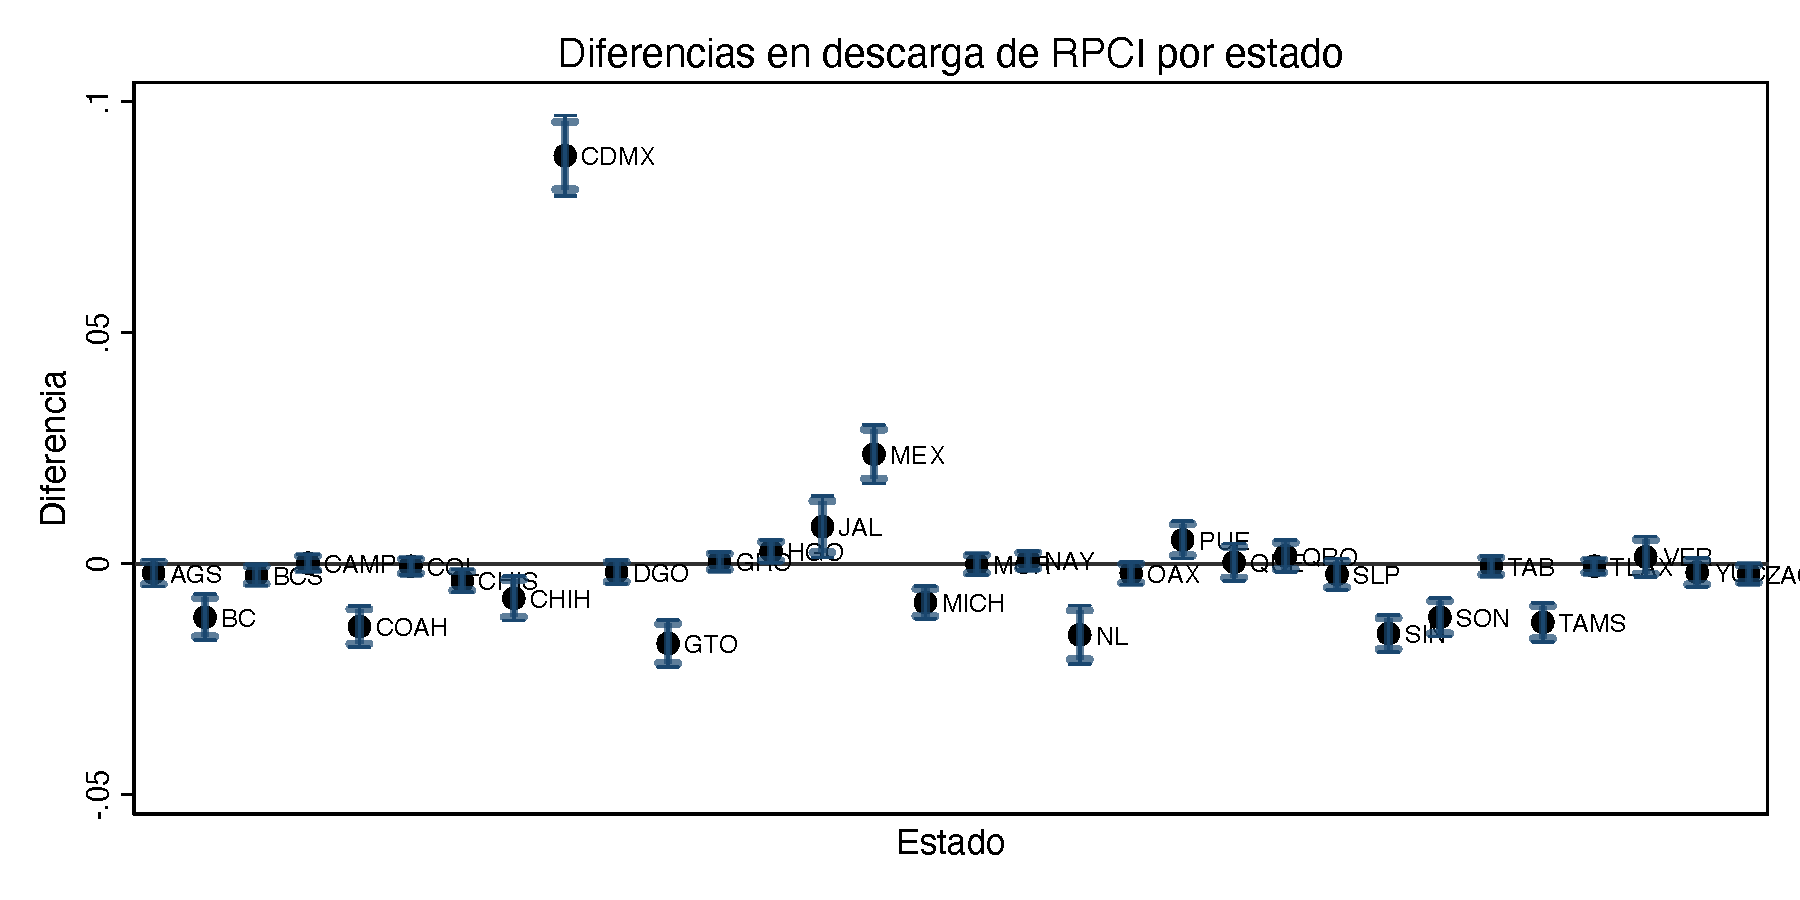
\includegraphics[width=\textwidth]{04_Figures/muestra_1porciento/balance_ent_final_graph.pdf}
%     \end{center}
% \end{figure}
% \scriptsize{
% \noindent Dado un estado, cada punto es el coeficiente resultante de correr la regresión $ent_{i} = T_{i} + \varepsilon$, donde $ent_{i}$ vale 1 si el trabajador laboraba en dicho estado en 2020, y $T_{i}$ vale 1 si el trabajador bajó el RPCI en algún momento. Es decir, dado un estado, cada punto en la figura representa la diferencia entre el porcentaje de trabajadores que bajaron el RPCI y laboran en dicho estado, y el porcentaje de trabajadores que no bajaron el RPCI y laboran en dicho estado. Por ejemplo, 25.2\% de los trabajadores que bajaron el RPCI son de CDMX, mientras que 16.4\% de los trabajadores que no bajaron el RPCI son de CDMX, por lo que la diferencia es de 8.8 pp.
% }

\begin{figure}[H]
    \caption{RPCI registers by month}
    \label{hist_download}
    \begin{center}
    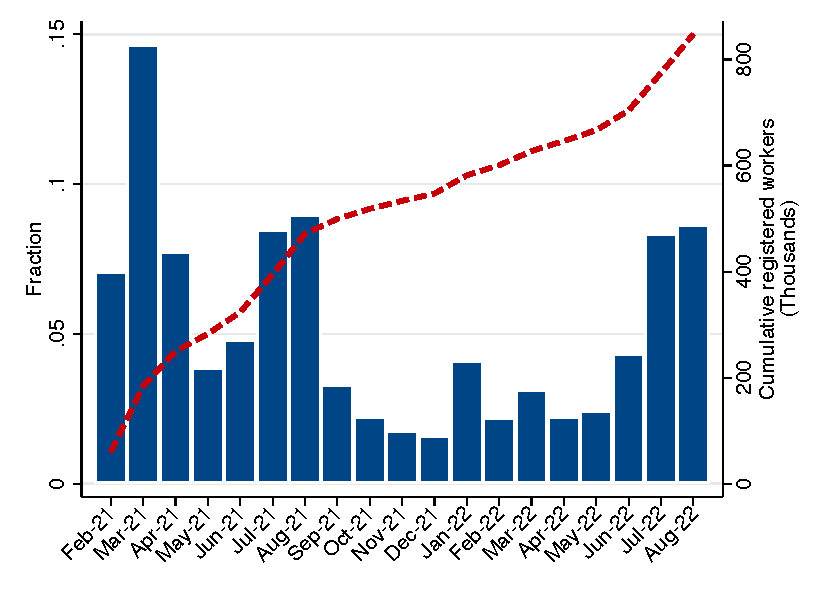
\includegraphics[width=0.75\textwidth]{04_Figures/muestra_1porciento/hist_download_month.pdf}
    \end{center}
\end{figure}
\scriptsize{
\noindent \textit{Sample:} 10\% of the workers registered at the Mexican Institute of Social Security (IMSS) between January 2020 and August 2022. The right y-axis measures the fraction of workers who registered for the RPCI during each month from the total workers who registered for the RPCI in the sample. The left y-axis measures the cumulative number of workers who registered for the RPCI in the sample.
}

\clearpage

\begin{figure}[H]
    \caption{Event studies - RPCI effect}
    \label{event_study}
    \begin{center}
    
    \begin{subfigure}{0.49\textwidth}
    \caption{Effect on wage}
    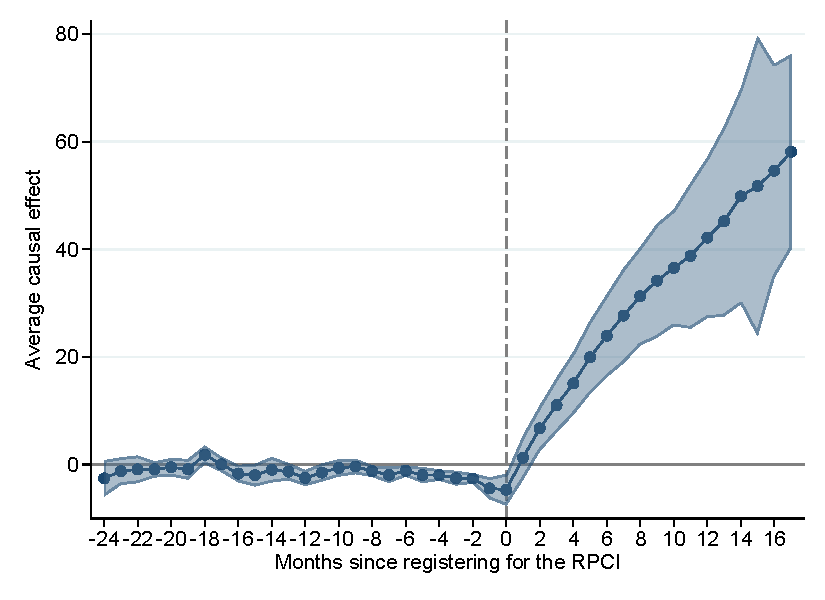
\includegraphics[width=\textwidth]{04_Figures/muestra_10porciento/event_study_sal_cierre_chaisemartin.pdf}
    \end{subfigure}
    \begin{subfigure}{0.49\textwidth}
    \caption{Effect on log wage}
    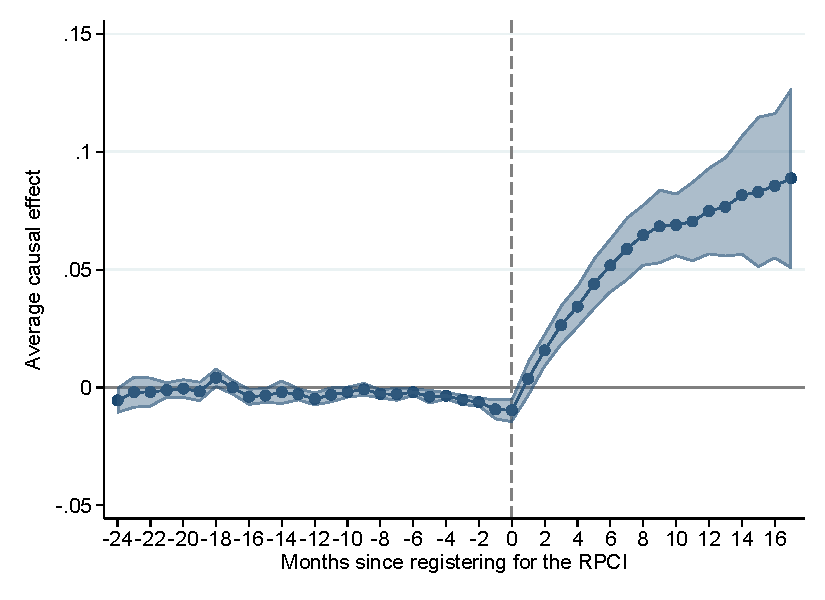
\includegraphics[width=\textwidth]{04_Figures/muestra_10porciento/event_study_log_sal_cierre_chaisemartin.pdf}
    \end{subfigure}
    
    \begin{subfigure}{0.49\textwidth}
    \caption{Effect on discharge}
    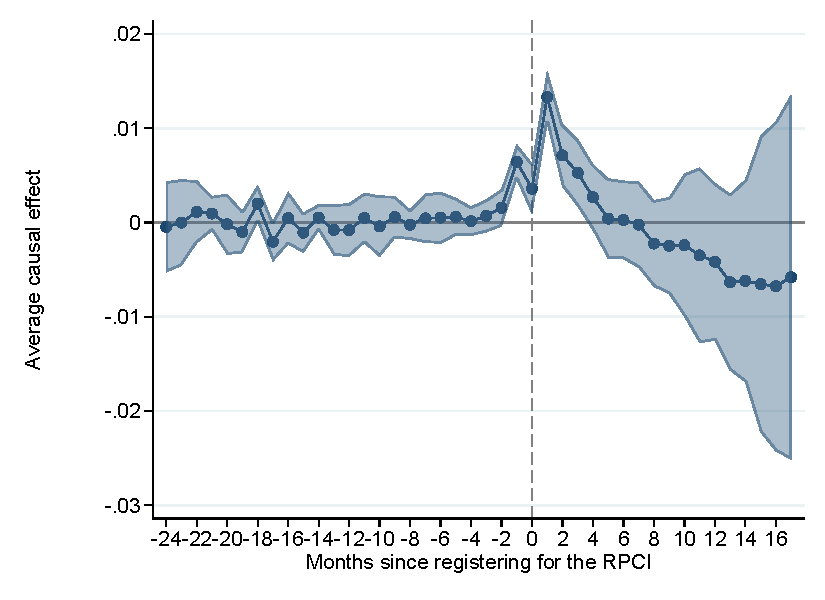
\includegraphics[width=\textwidth]{04_Figures/muestra_10porciento/event_study_baja_cierre_chaisemartin.pdf}
    \end{subfigure}
    \begin{subfigure}{0.49\textwidth}
    \caption{Effect on permanent discharge}
    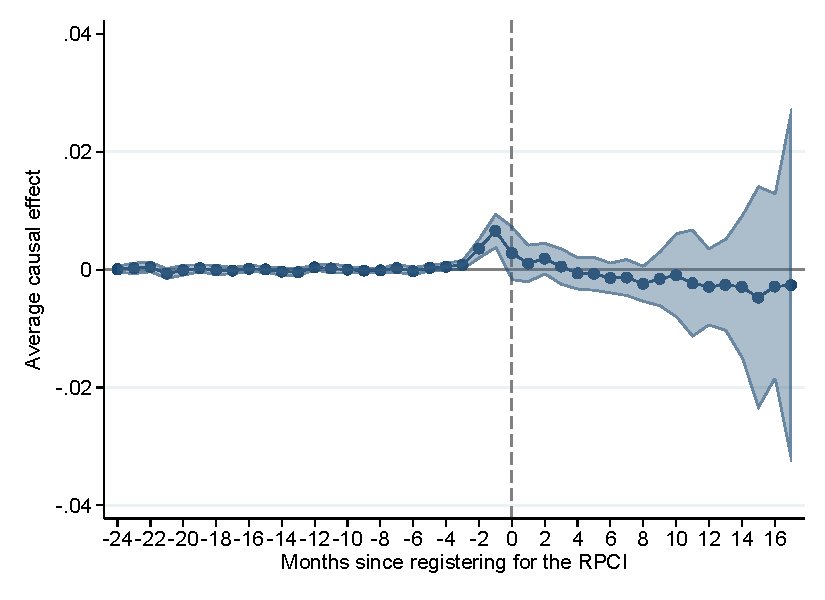
\includegraphics[width=\textwidth]{04_Figures/muestra_10porciento/event_study_baja_permanente_chaisemartin.pdf}
    \end{subfigure}
    
    \begin{subfigure}{0.49\textwidth}
    \caption{Effect on job change}
    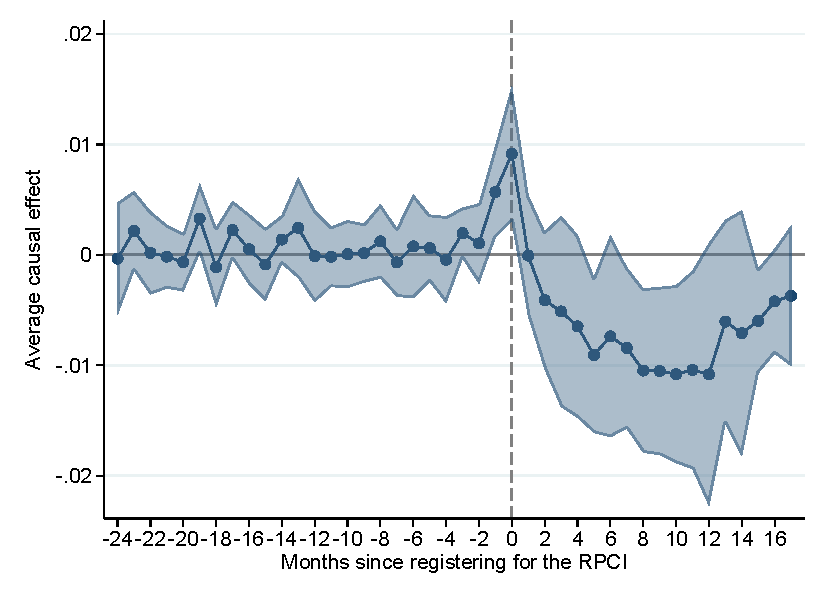
\includegraphics[width=\textwidth]{04_Figures/muestra_10porciento/event_study_cambio_cierre_chaisemartin.pdf}
    \end{subfigure}
    
    %\textit{Do file: did_multiplegt_rpci.do}
    \end{center}
\end{figure}
\scriptsize{
\noindent \textit{Sample:} 10\% of the workers registered at the Mexican Institute of Social Security (IMSS) between January 2020 and August 2022. The graphs use the estimators proposed by Chaisemartin and D'Haultfoeuille to prevent posible negative weights in the Difference in Differences estimators.
}

\clearpage

\begin{figure}[H]
    \caption{Workers by the number of months observed after registering for the RPCI}
    \label{hist_time_since_treated}
    \begin{center}
    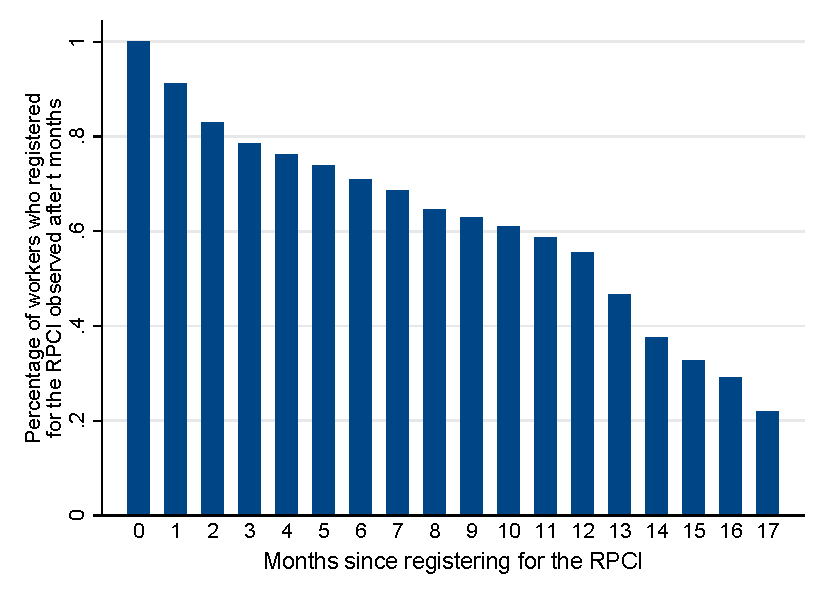
\includegraphics[width=0.5\textwidth]{04_Figures/muestra_10porciento/hist_time_since_treated.pdf}
    \end{center}
\end{figure}
\scriptsize{
\noindent \textit{Sample:} 10\% of the workers registered at the Mexican Institute of Social Security (IMSS) between January 2020 and August 2022. Not all workers registered for the RPCI at the same time, so not all workers are observed the same number of months after registering for the RPCI in the sample. The y-axis measures the percentage of workers observed $t$ months after registering for the RPCI from the total number of workers who registered for the RPCI.
}

\clearpage

\begin{figure}[H]
    \caption{Percentage of workers having the same wage after the RPCI}
    \label{hist_wage_time_since_treated}
    \begin{center}
    
    \begin{subfigure}{0.49\textwidth}
    \caption{Treatment: after registering for the RPCI}
    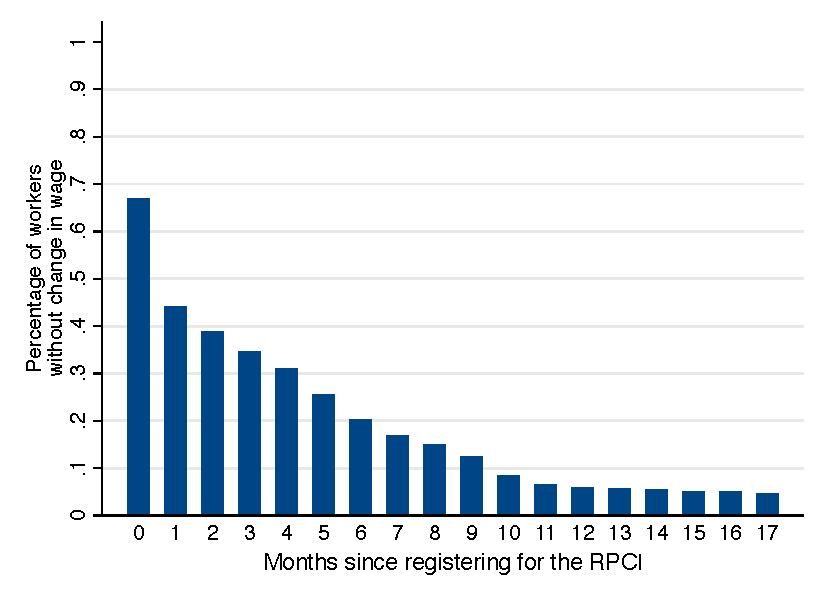
\includegraphics[width=\textwidth]{04_Figures/muestra_1porciento/hist_wage_time_since_treated_treat.pdf}
    \end{subfigure}
    \begin{subfigure}{0.49\textwidth}
    \caption{Control: after the RPCI launch}
    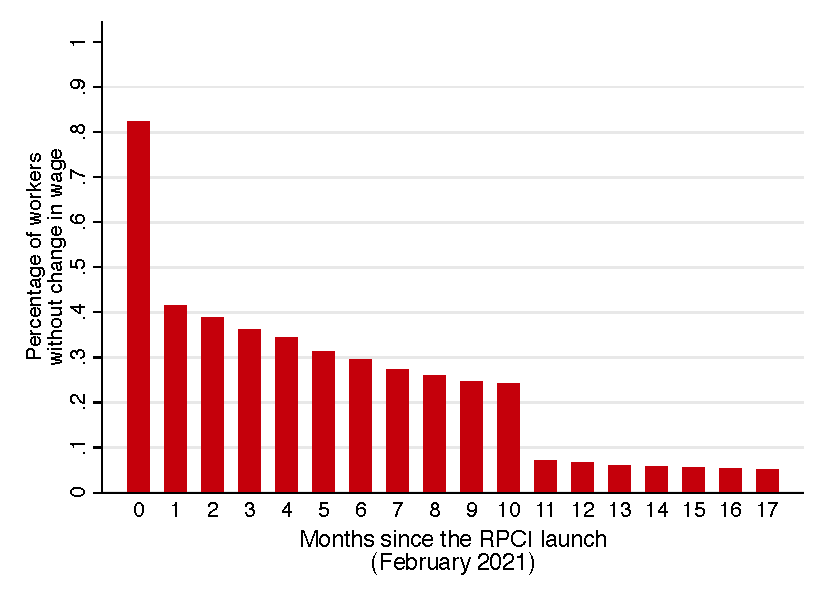
\includegraphics[width=\textwidth]{04_Figures/muestra_1porciento/hist_wage_time_since_treated_control.pdf}
    \end{subfigure}
    
    %\textit{Do file: twfe_beta_cohort_rpci.do}
    \end{center}
\end{figure}
\scriptsize{
\noindent This figures plot the percentage of workers that have the same wage after $t$ months. \textit{Sample:} 1\% of the workers registered at the Mexican Institute of Social Security (IMSS) between January 2020 and August 2022. For the treatment group, compares the wage the worker had one month before registering for the RPCI with the wage after $t$ months of the register. For the control group, compares the wage of January 2021, the month before the RPCI launch, with the wage $t$ months after. The y-axis measures the percentage of workers observed $t$ months with the same wage as in $t = -1$.
\todo[inline]{Marco: I should repeat this figure after having the matched data, since the control figure has clear seasonality. I'll match on baseline characteristics and compare each control and treatment pair for the same monthly periods. Still, after one month, the treatments change more their wage than the controls}
}


\clearpage

\begin{figure}[H]
    \caption{RPCI effect by cohort}
    \label{twfe_beta_cohort}
    \begin{center}
    
    \begin{subfigure}{0.49\textwidth}
    \caption{Effect on wage}
    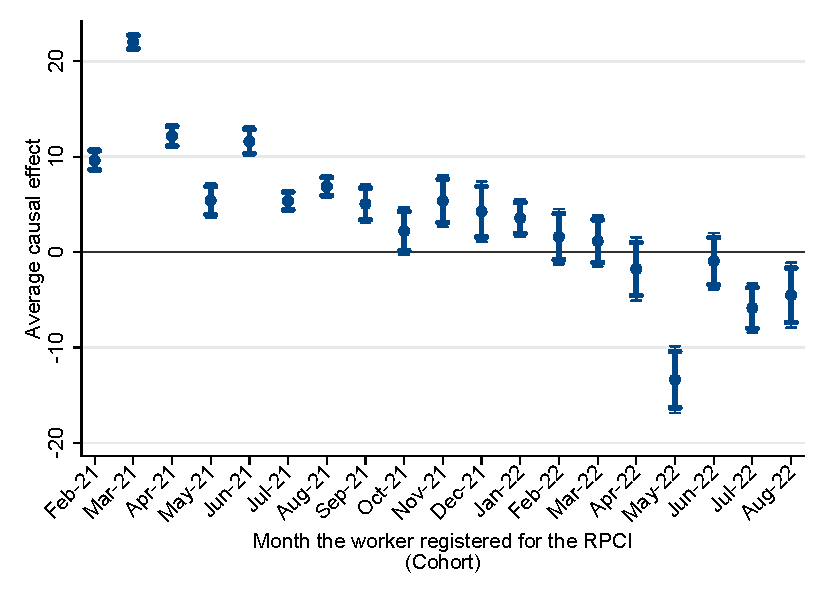
\includegraphics[width=\textwidth]{04_Figures/muestra_10porciento/twfe_beta_cohort_sal_cierre.pdf}
    \end{subfigure}
    \begin{subfigure}{0.49\textwidth}
    \caption{Effect on log wage}
    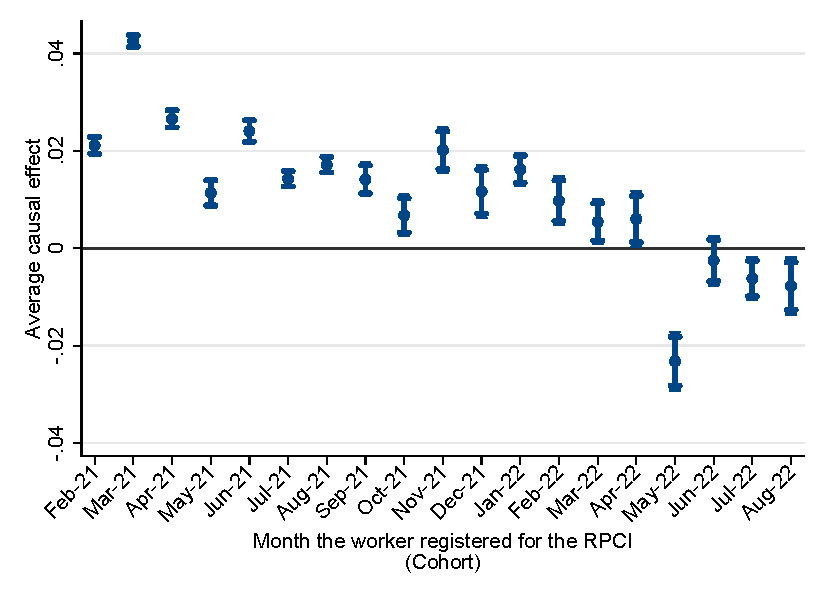
\includegraphics[width=\textwidth]{04_Figures/muestra_10porciento/twfe_beta_cohort_log_sal_cierre.pdf}
    \end{subfigure}
    
    %\textit{Do file: twfe_beta_cohort_rpci.do}
    \end{center}
\end{figure}
\scriptsize{
\noindent \textit{Sample:} 10\% of the workers registered at the Mexican Institute of Social Security (IMSS) between January 2020 and August 2022. Each point in the graph corresponds to the estimated regression coefficient where the sample conditions the treatment group by the cohort of register for the RPCI. All regressions have the same control group, meaning all samples include the workers who never registered for the RPCI. Regressions use the TWFE specification $y_{it} = \gamma_{i} + \theta_{t}+ \beta RPCI_{it} +\epsilon_{it}$, where $\gamma_{i}$ are dummies for each worker id, $\theta_{t}$ are dummies for each monthly period, and $RPCI_{it}$ are dummies where 1 means that the worker registered for the RPCI during that month or previous month, and include dummies for each state and dummies for each wage decile of the wage distribution during 2020, both interacted with dummies for each quarterly period. 
}

\begin{figure}[H]
    \caption{Event studies - RPCI effect on wage by cohort}
    \label{event_study_cohort}
    \begin{center}
    
    \begin{subfigure}{0.49\textwidth}
    \caption{Early adopters}
    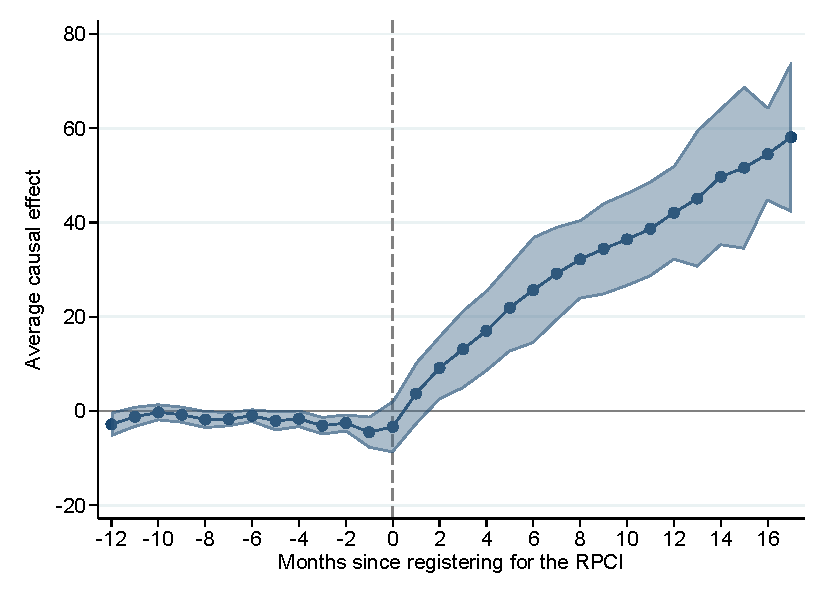
\includegraphics[width=\textwidth]{04_Figures/muestra_10porciento/event_study_sal_cierre_chaisemartin_adopters_early.pdf}
    \end{subfigure}
    \begin{subfigure}{0.49\textwidth}
    \caption{Late adopters}
    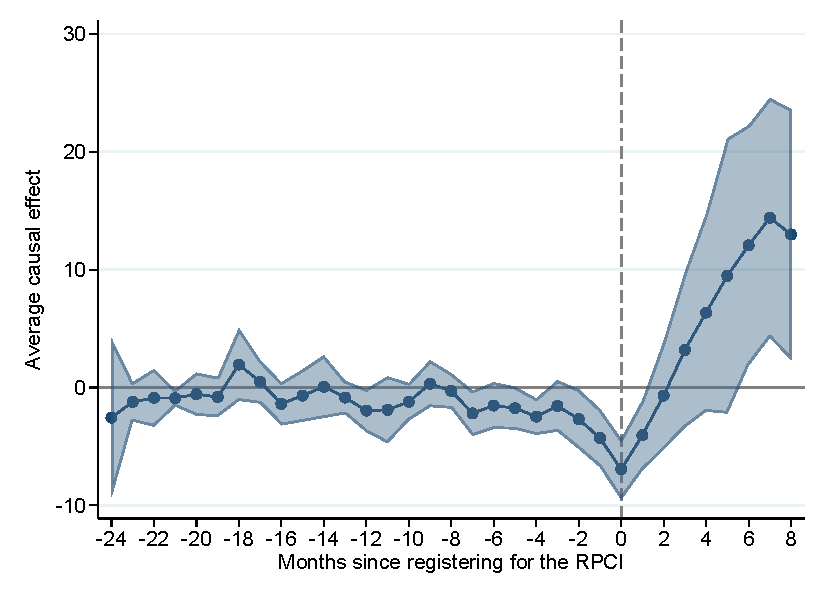
\includegraphics[width=\textwidth]{04_Figures/muestra_10porciento/event_study_sal_cierre_chaisemartin_adopters_late.pdf}
    \end{subfigure}
    
    %\textit{Do file: did_multiplegt_heterogeneity_rpci.do}
    \end{center}
\end{figure}
\scriptsize{
\noindent \textit{Sample:} 10\% of the workers registered at the Mexican Institute of Social Security (IMSS) between January 2020 and August 2022. The graphs use the estimators proposed by Chaisemartin and D'Haultfoeuille to prevent posible negative weights in the Difference in Differences estimators. Each subfigure conditions the treatment group by the cohort of register for the RPCI. Subfigure (a) conditions the treatment group to early adopters, meaning the workers who registered for the RPCI during the first nine months after the RPCI launch (February 2021 to October 2021). Subfigure (b) conditions the treatment group to late adopters, meaning the workers who registered for the RPCI during the next nine months (November 2021 to August 2022). Both subfigures have the same control group, meaning the workers who never registered for the RPCI.
}

\clearpage

\begin{figure}[H]
    \caption{Event studies - RPCI effect on wage by worker characteristics}
    \label{event_study_worker_characteristics}
    \begin{center}
    
    \begin{subfigure}{0.49\textwidth}
    \caption{Men}
    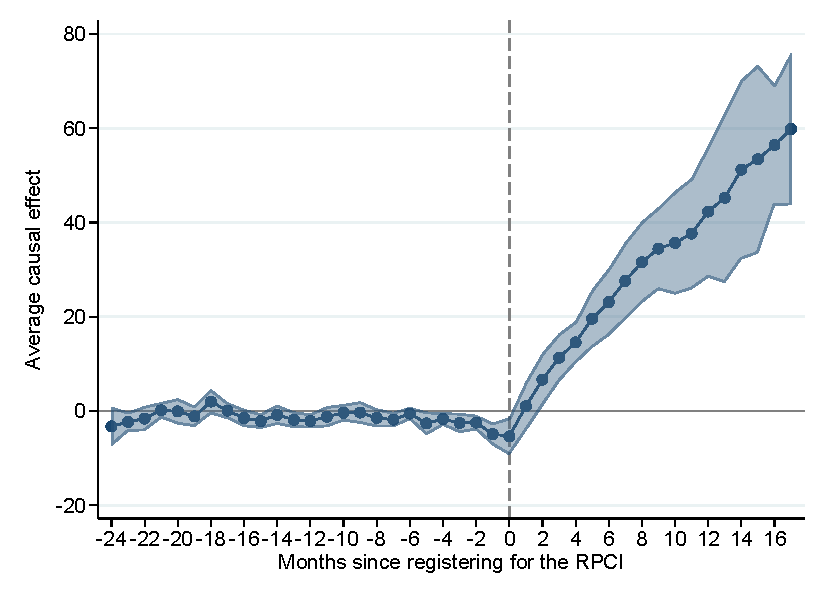
\includegraphics[width=\textwidth]{04_Figures/muestra_10porciento/event_study_sal_cierre_chaisemartin_sexo_0.pdf}
    \end{subfigure}
    \begin{subfigure}{0.49\textwidth}
    \caption{Woman}
    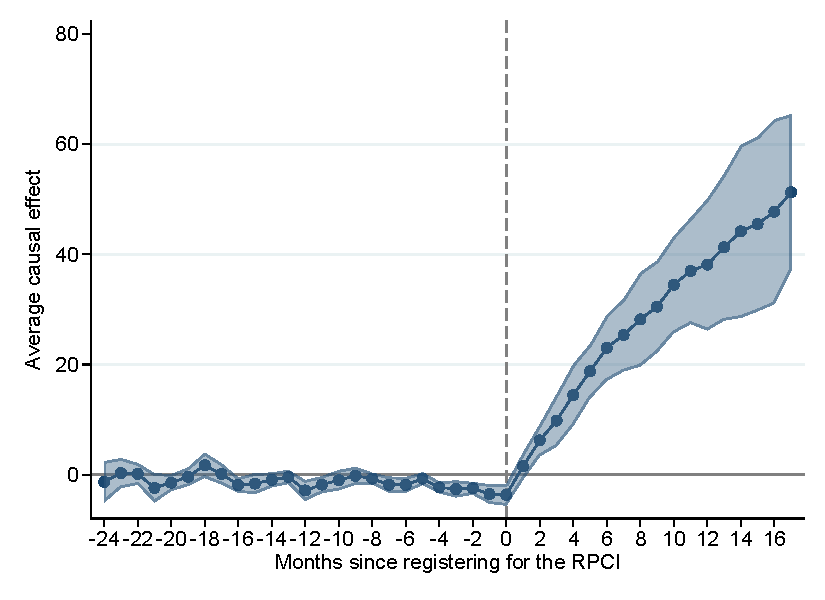
\includegraphics[width=\textwidth]{04_Figures/muestra_10porciento/event_study_sal_cierre_chaisemartin_sexo_1.pdf}
    \end{subfigure}
    
    \begin{subfigure}{0.49\textwidth}
    \caption{Outsourcing}
    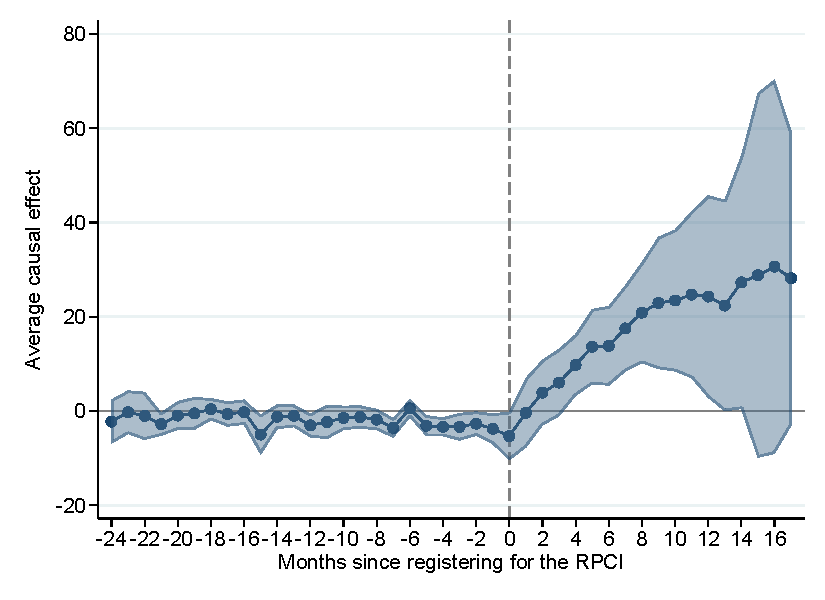
\includegraphics[width=\textwidth]{04_Figures/muestra_10porciento/event_study_sal_cierre_chaisemartin_outsourcing.pdf}
    \end{subfigure}
    \begin{subfigure}{0.49\textwidth}
    \caption{Temporary}
    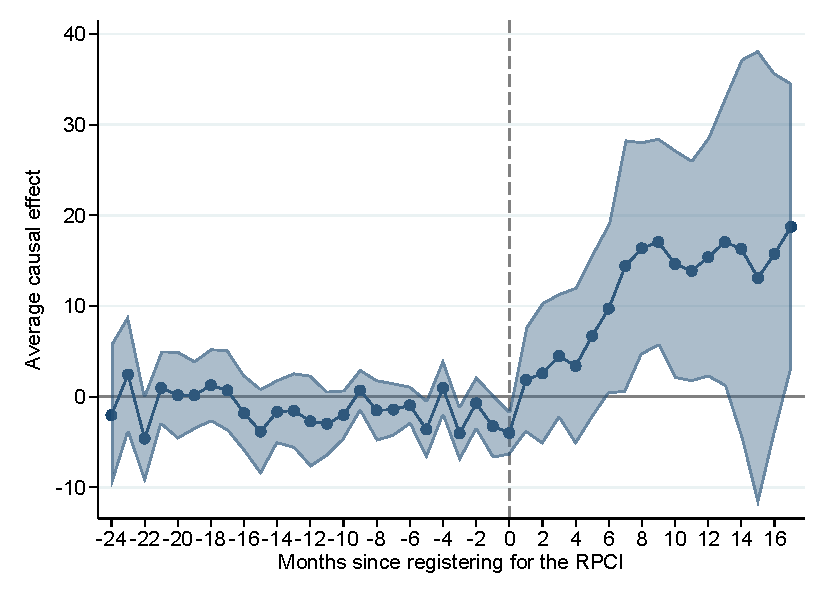
\includegraphics[width=\textwidth]{04_Figures/muestra_10porciento/event_study_sal_cierre_chaisemartin_eventual.pdf}
    \end{subfigure}
    
    %\textit{Do file: did_multiplegt_heterogeneity_rpci.do}
    \end{center}
\end{figure}
\scriptsize{
\noindent \textit{Sample:} 10\% of the workers registered at the Mexican Institute of Social Security (IMSS) between January 2020 and August 2022. The graphs use the estimators proposed by Chaisemartin and D'Haultfoeuille to prevent posible negative weights in the Difference in Differences estimators. Each subfigure conditions on a worker characteristics at baseline, during 2020, previous to the RPCI launch. Subfigures (a) and (b) condition on the worker gender. Subfigure (c) conditions on workers hired through outsourcing. Subfigure (d) conditions on temporary workers.
}

\clearpage

\begin{figure}[H]
    \caption{Event studies - RPCI effect on wage by firm characteristics}
    \label{event_study_firm_characteristics}
    \begin{center}
    
    \begin{subfigure}{0.49\textwidth}
    \caption{Transformation Industry}
    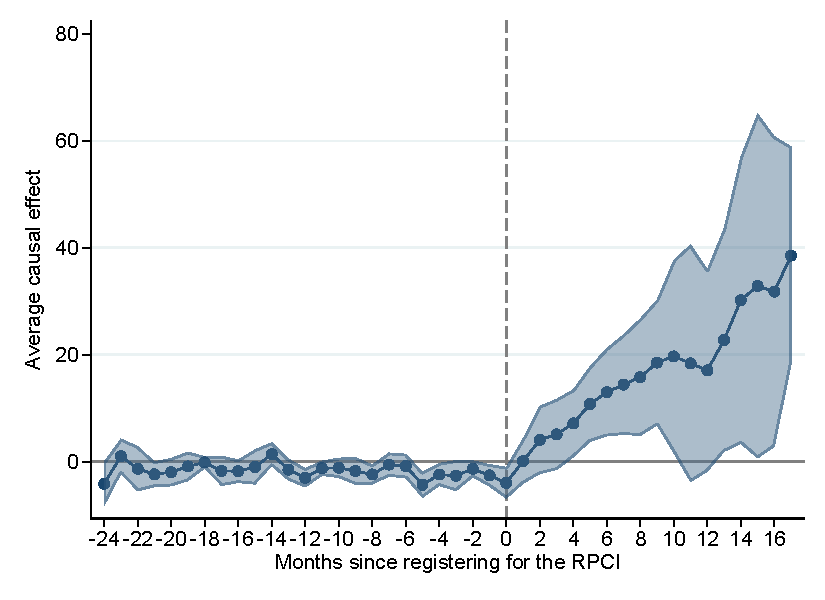
\includegraphics[width=\textwidth]{04_Figures/muestra_10porciento/event_study_sal_cierre_chaisemartin_div_final_3.pdf}
    \end{subfigure}
    \begin{subfigure}{0.49\textwidth}
    \caption{Construction Industry}
    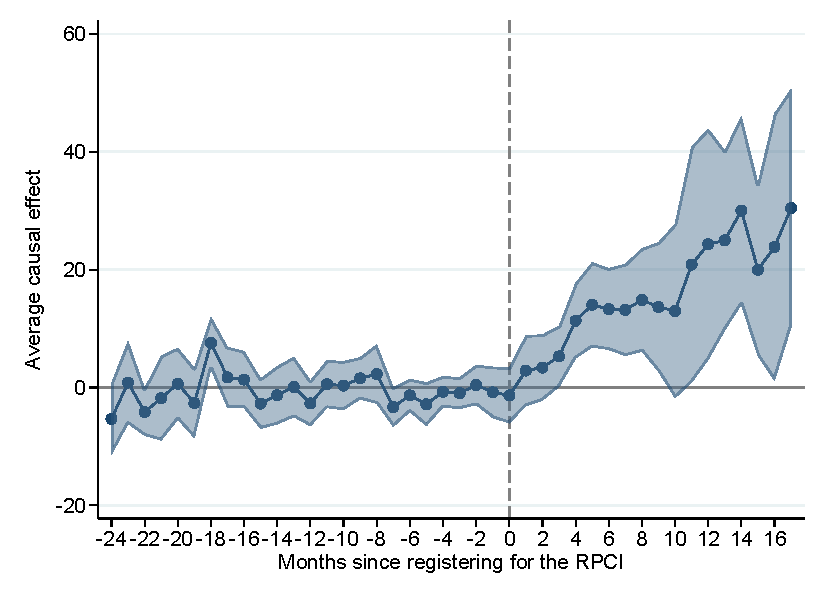
\includegraphics[width=\textwidth]{04_Figures/muestra_10porciento/event_study_sal_cierre_chaisemartin_div_final_4.pdf}
    \end{subfigure}
    
    \begin{subfigure}{0.49\textwidth}
    \caption{Commerce}
    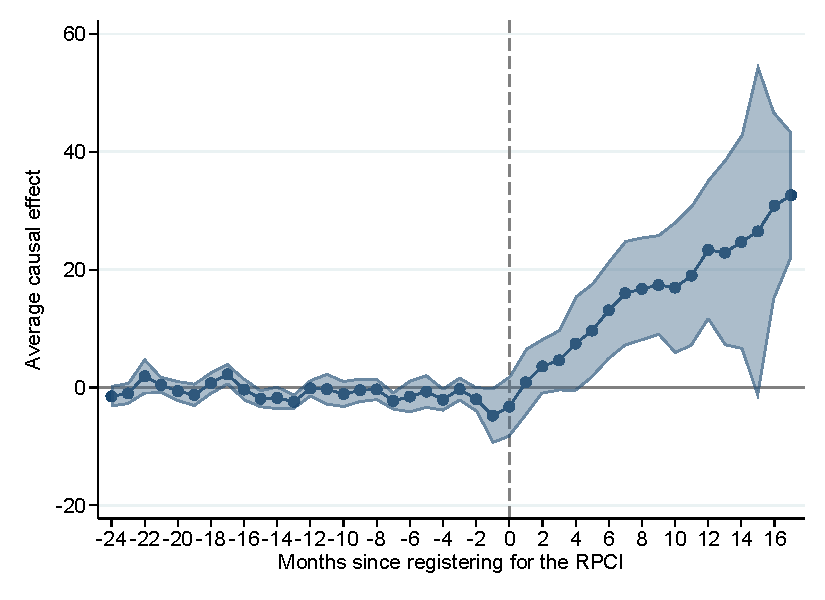
\includegraphics[width=\textwidth]{04_Figures/muestra_10porciento/event_study_sal_cierre_chaisemartin_div_final_6.pdf}
    \end{subfigure}
    \begin{subfigure}{0.49\textwidth}
    \caption{Communications and Transportation}
    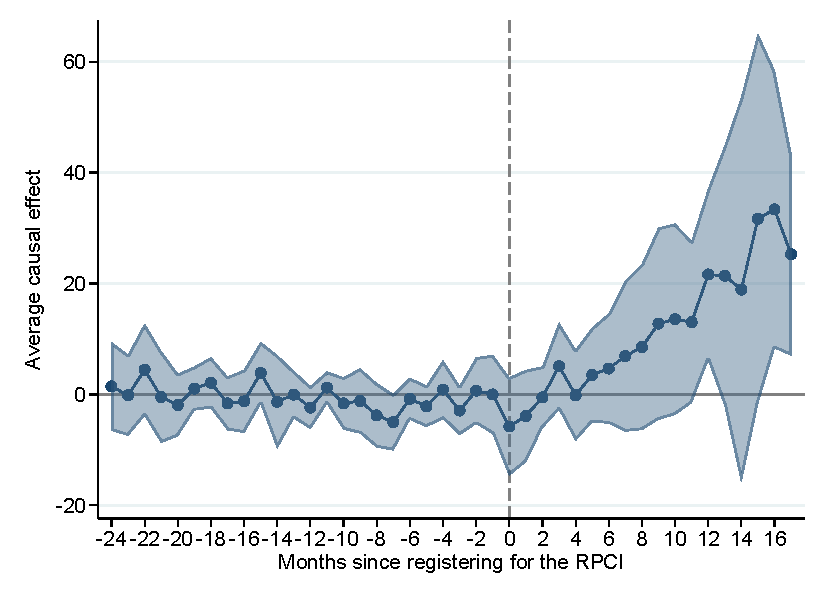
\includegraphics[width=\textwidth]{04_Figures/muestra_10porciento/event_study_sal_cierre_chaisemartin_div_final_7.pdf}
    \end{subfigure}
    
    %\textit{Do file: did_multiplegt_heterogeneity_rpci.do}
    \end{center}
\end{figure}
\scriptsize{
\noindent \textit{Sample:} 10\% of the workers registered at the Mexican Institute of Social Security (IMSS) between January 2020 and August 2022. The graphs use the estimators proposed by Chaisemartin and D'Haultfoeuille to prevent posible negative weights in the Difference in Differences estimators. Each subfigure conditions on firm characteristics at baseline, during 2020, previous to the RPCI launch. Columns (a) to (f) condition on the firm industry: (a) transformation industry, (b) construction industry, (c) commerce, (d) communications and transportation, (e) services for firms and people, (f) communal and social services. Column (g) and (h) condition on firm size categories: (g) small firms (less than 250 workers), (h) big firms (more than 1000 workers).
}

\clearpage

\begin{figure}[H]
    \ContinuedFloat
    \caption{(Continued) Event studies - RPCI effect on wage by firm characteristics}
    \label{event_study_firm_characteristics_cont}
    \begin{center}

    \begin{subfigure}{0.49\textwidth}
    \caption{Services for Firms and People}
    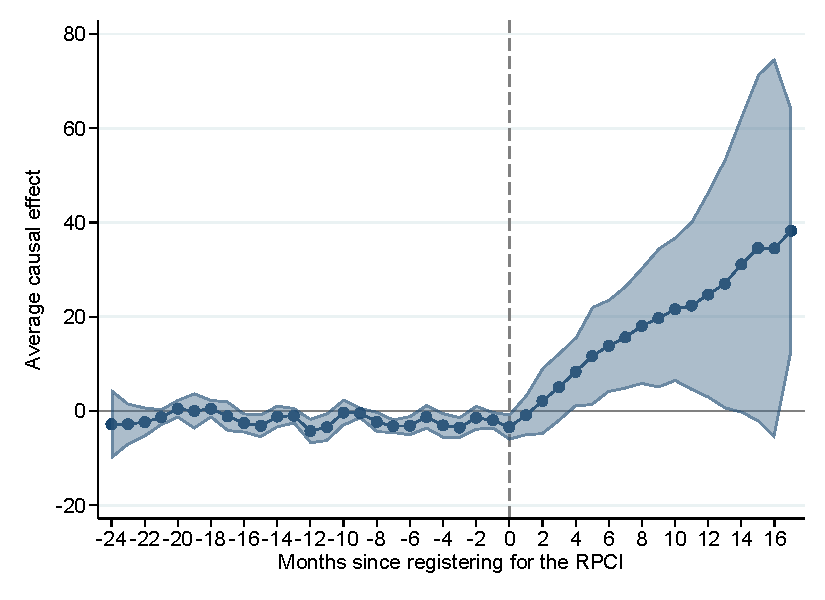
\includegraphics[width=\textwidth]{04_Figures/muestra_10porciento/event_study_sal_cierre_chaisemartin_div_final_8.pdf}
    \end{subfigure}
    \begin{subfigure}{0.49\textwidth}
    \caption{Social and Communal Services}
    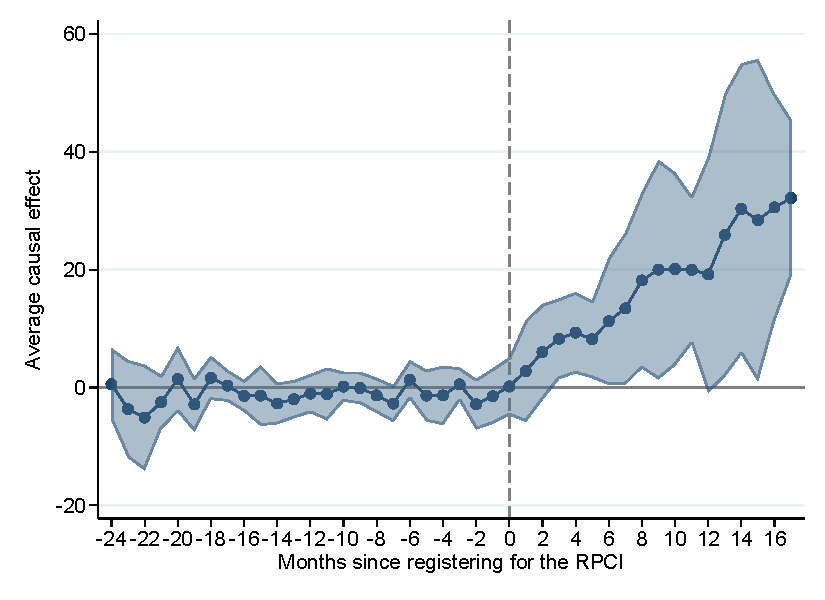
\includegraphics[width=\textwidth]{04_Figures/muestra_10porciento/event_study_sal_cierre_chaisemartin_div_final_9.pdf}
    \end{subfigure}
    
    \begin{subfigure}{0.49\textwidth}
    \caption{Small Firms}
    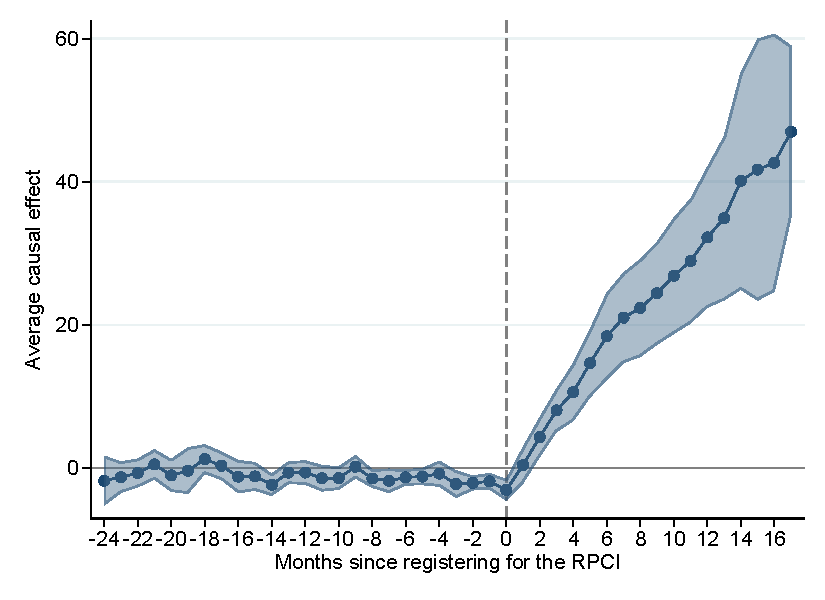
\includegraphics[width=\textwidth]{04_Figures/muestra_10porciento/event_study_sal_cierre_chaisemartin_pyme.pdf}
    \end{subfigure}
    \begin{subfigure}{0.49\textwidth}
    \caption{Big Firms}
    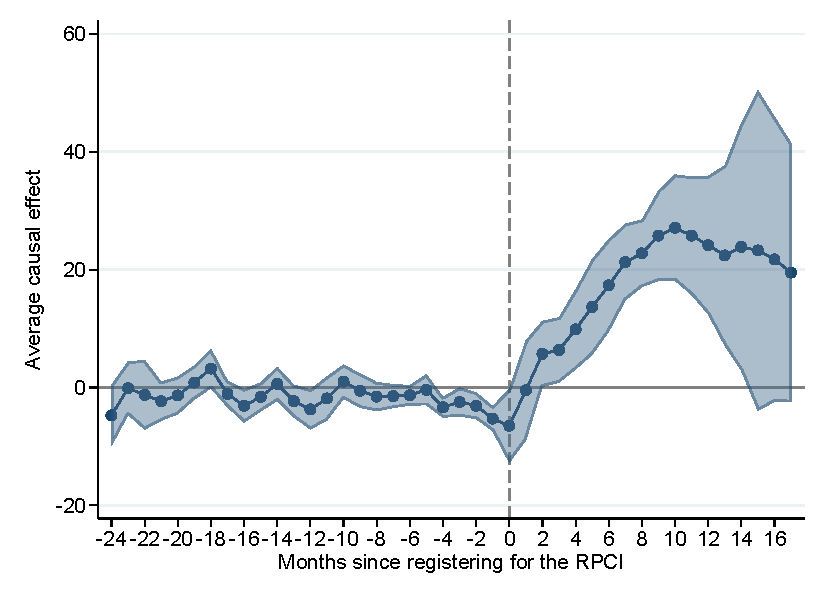
\includegraphics[width=\textwidth]{04_Figures/muestra_10porciento/event_study_sal_cierre_chaisemartin_emp_grande.pdf}
    \end{subfigure}
    
    %\textit{Do file: did_multiplegt_heterogeneity_rpci.do}
    \end{center}
\end{figure}

\scriptsize{
\noindent \textit{Sample:} 10\% of the workers registered at the Mexican Institute of Social Security (IMSS) between January 2020 and August 2022. The graphs use the estimators proposed by Chaisemartin and D'Haultfoeuille to prevent posible negative weights in the Difference in Differences estimators. Each subfigure conditions on firm characteristics at baseline, during 2020, previous to the RPCI launch. Subfigures (a) to (f) condition on the firm industry: (a) transformation industry, (b) construction industry, (c) commerce, (d) communications and transportation, (e) services for firms and people, (f) communal and social services. Subfigures (g) and (h) condition on firm size categories: (g) small firms (less than 250 workers), (h) big firms (more than 1000 workers).
}

\clearpage

\begin{figure}[H]
    \caption{Event studies - RPCI effect on wage by firm size}
    \label{event_study_firm_size}
    \begin{center}
    
    \begin{subfigure}{0.49\textwidth}
    \caption{1 Job}
    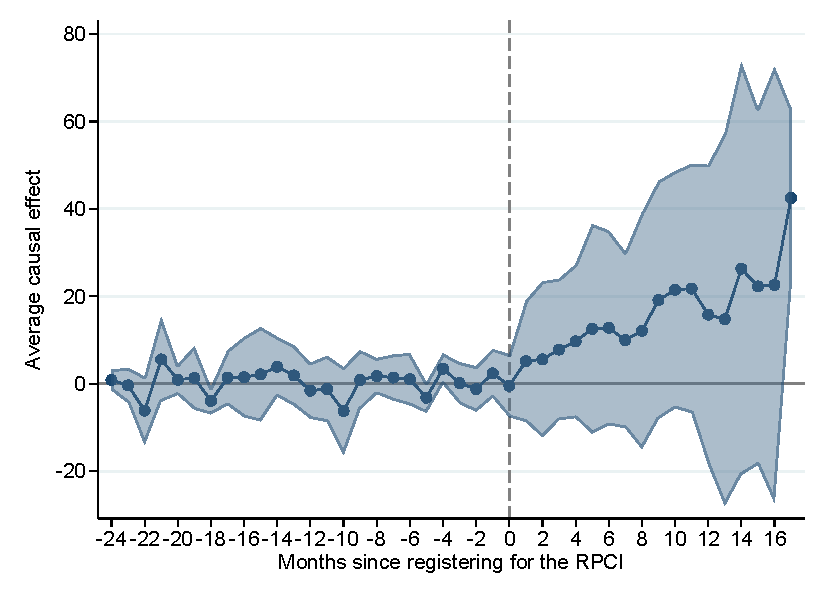
\includegraphics[width=\textwidth]{04_Figures/muestra_10porciento/event_study_sal_cierre_chaisemartin_firm_size_1.pdf}
    \end{subfigure}
    \begin{subfigure}{0.49\textwidth}
    \caption{2 to 5 Jobs}
    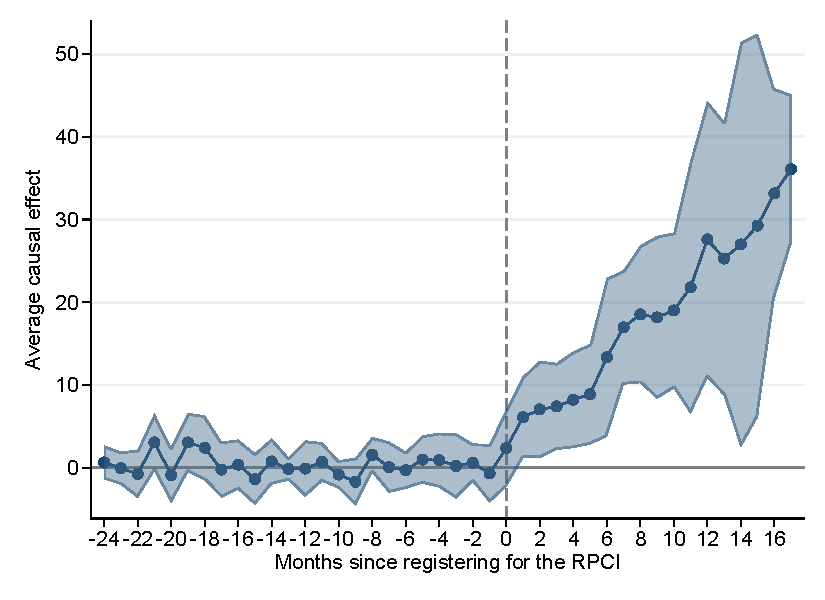
\includegraphics[width=\textwidth]{04_Figures/muestra_10porciento/event_study_sal_cierre_chaisemartin_firm_size_2.pdf}
    \end{subfigure}
    
    \begin{subfigure}{0.49\textwidth}
    \caption{6 to 50 Jobs}
    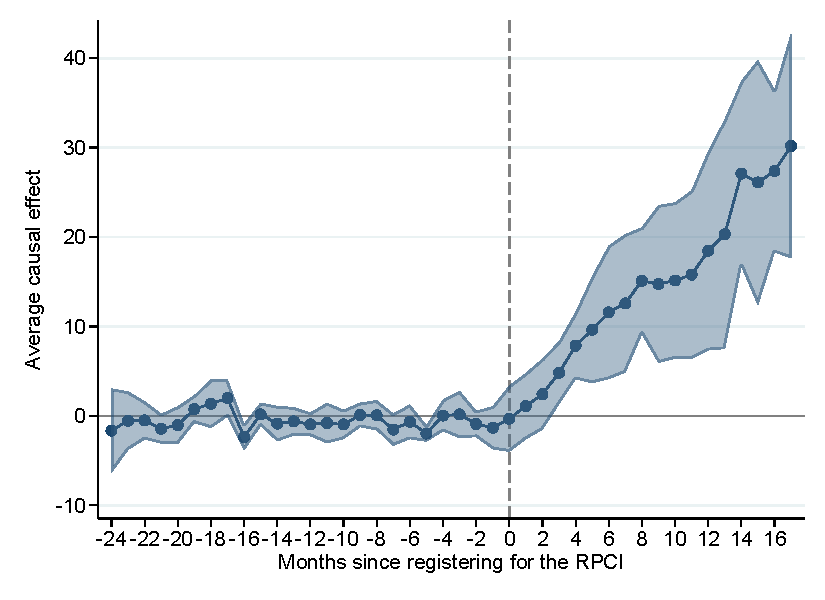
\includegraphics[width=\textwidth]{04_Figures/muestra_10porciento/event_study_sal_cierre_chaisemartin_firm_size_3.pdf}
    \end{subfigure}
    \begin{subfigure}{0.49\textwidth}
    \caption{51 to 250 Jobs}
    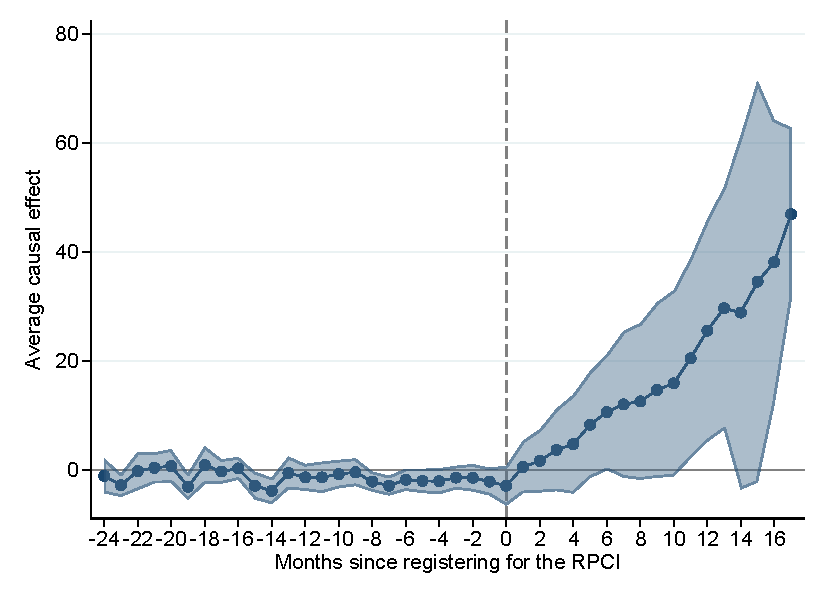
\includegraphics[width=\textwidth]{04_Figures/muestra_10porciento/event_study_sal_cierre_chaisemartin_firm_size_4.pdf}
    \end{subfigure}
    
    %\textit{Do file: did_multiplegt_heterogeneity_rpci.do}
    \end{center}
\end{figure}
\scriptsize{
\noindent \textit{Sample:} 10\% of the workers registered at the Mexican Institute of Social Security (IMSS) between January 2020 and August 2022. The graphs use the estimators proposed by Chaisemartin and D'Haultfoeuille to prevent posible negative weights in the Difference in Differences estimators.  Each subfigure conditions on firm size at baseline, during 2020, previous to the RPCI launch: (a) 1 job, (b) 2 to 5 jobs, (c) 6 to 50 jobs, (d) 51 to 250 jobs, (e) 251 to 500 jobs, (f) 501 to 1000 jobs, (g) more than 1000 jobs.
}


\clearpage

\begin{figure}[H]
    \ContinuedFloat
    \caption{(Continued) Event studies - RPCI effect on wage by firm characteristics}
    \label{event_study_firm_size_cont}
    \begin{center}

    \begin{subfigure}{0.49\textwidth}
    \caption{251 to 500 Jobs}
    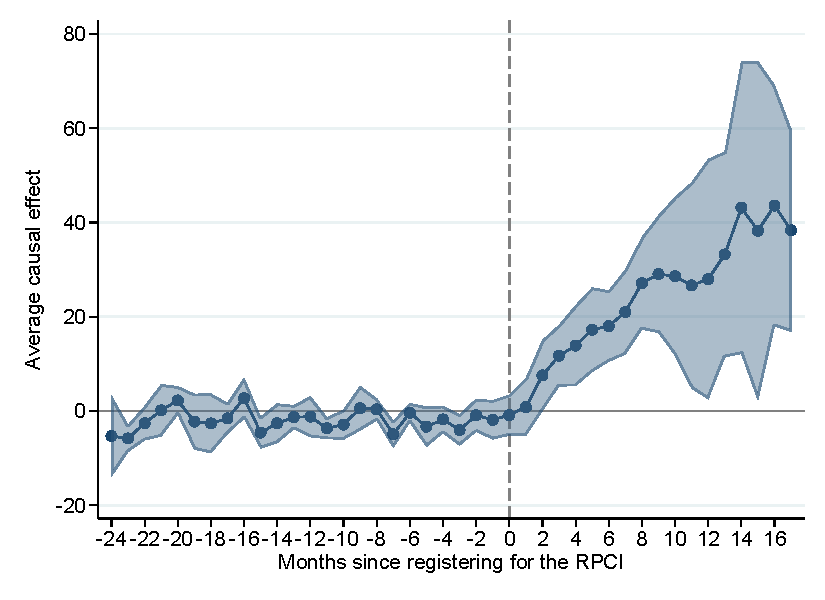
\includegraphics[width=\textwidth]{04_Figures/muestra_10porciento/event_study_sal_cierre_chaisemartin_firm_size_5.pdf}
    \end{subfigure}
    \begin{subfigure}{0.49\textwidth}
    \caption{501 to 1000 Jobs}
    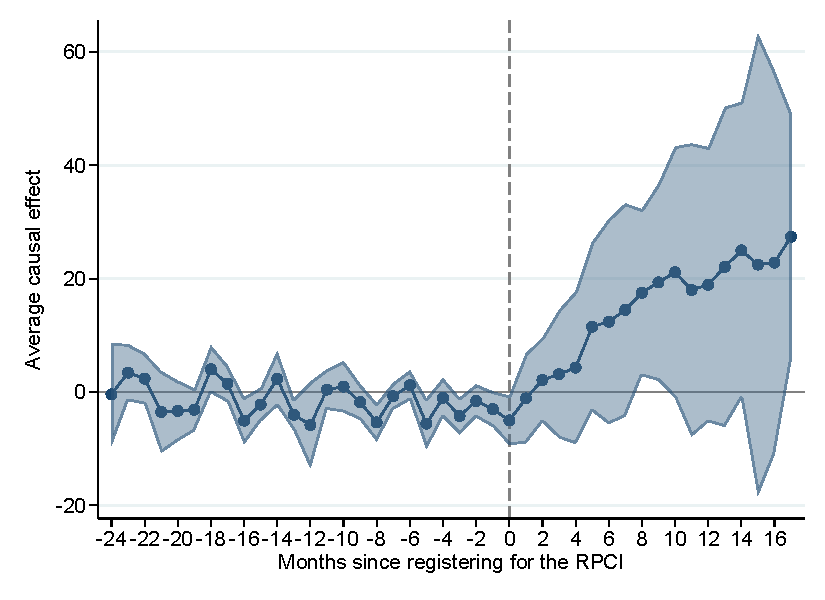
\includegraphics[width=\textwidth]{04_Figures/muestra_10porciento/event_study_sal_cierre_chaisemartin_firm_size_6.pdf}
    \end{subfigure}
    
    \begin{subfigure}{0.49\textwidth}
    \caption{1000+ Jobs}
    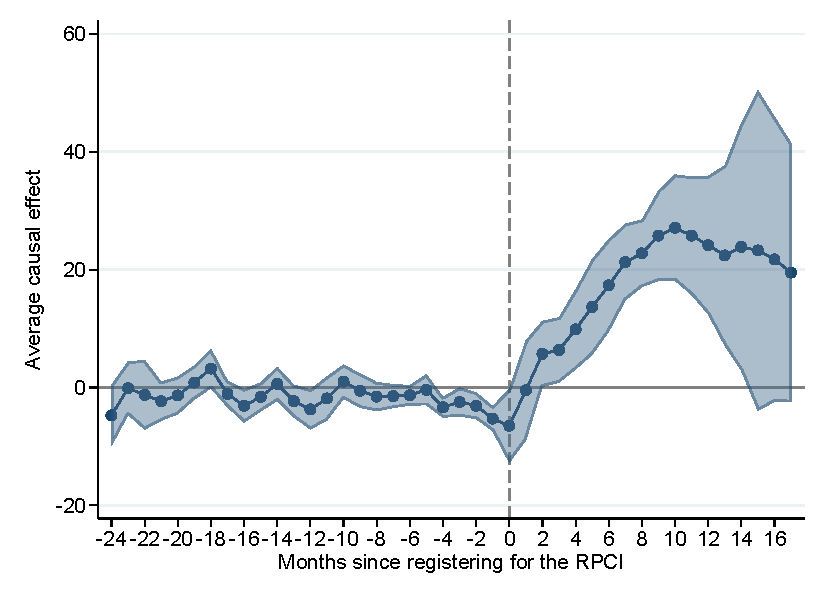
\includegraphics[width=\textwidth]{04_Figures/muestra_10porciento/event_study_sal_cierre_chaisemartin_firm_size_7.pdf}
    \end{subfigure}
    
    %\textit{Do file: did_multiplegt_heterogeneity_rpci.do}
    \end{center}
\end{figure}

\scriptsize{
\noindent \textit{Sample:} 10\% of the workers registered at the Mexican Institute of Social Security (IMSS) between January 2020 and August 2022. The graphs use the estimators proposed by Chaisemartin and D'Haultfoeuille to prevent posible negative weights in the Difference in Differences estimators.  Each subfigure conditions on firm size at baseline, during 2020, previous to the RPCI launch: (a) 1 job, (b) 2 to 5 jobs, (c) 6 to 50 jobs, (d) 51 to 250 jobs, (e) 251 to 500 jobs, (f) 501 to 1000 jobs, (g) more than 1000 jobs.
}

\clearpage

\begin{figure}[H]
    \caption{Worker Survey Graphs}
    \label{worker_surver_1}
    \begin{center}

    \begin{subfigure}{0.49\textwidth}
    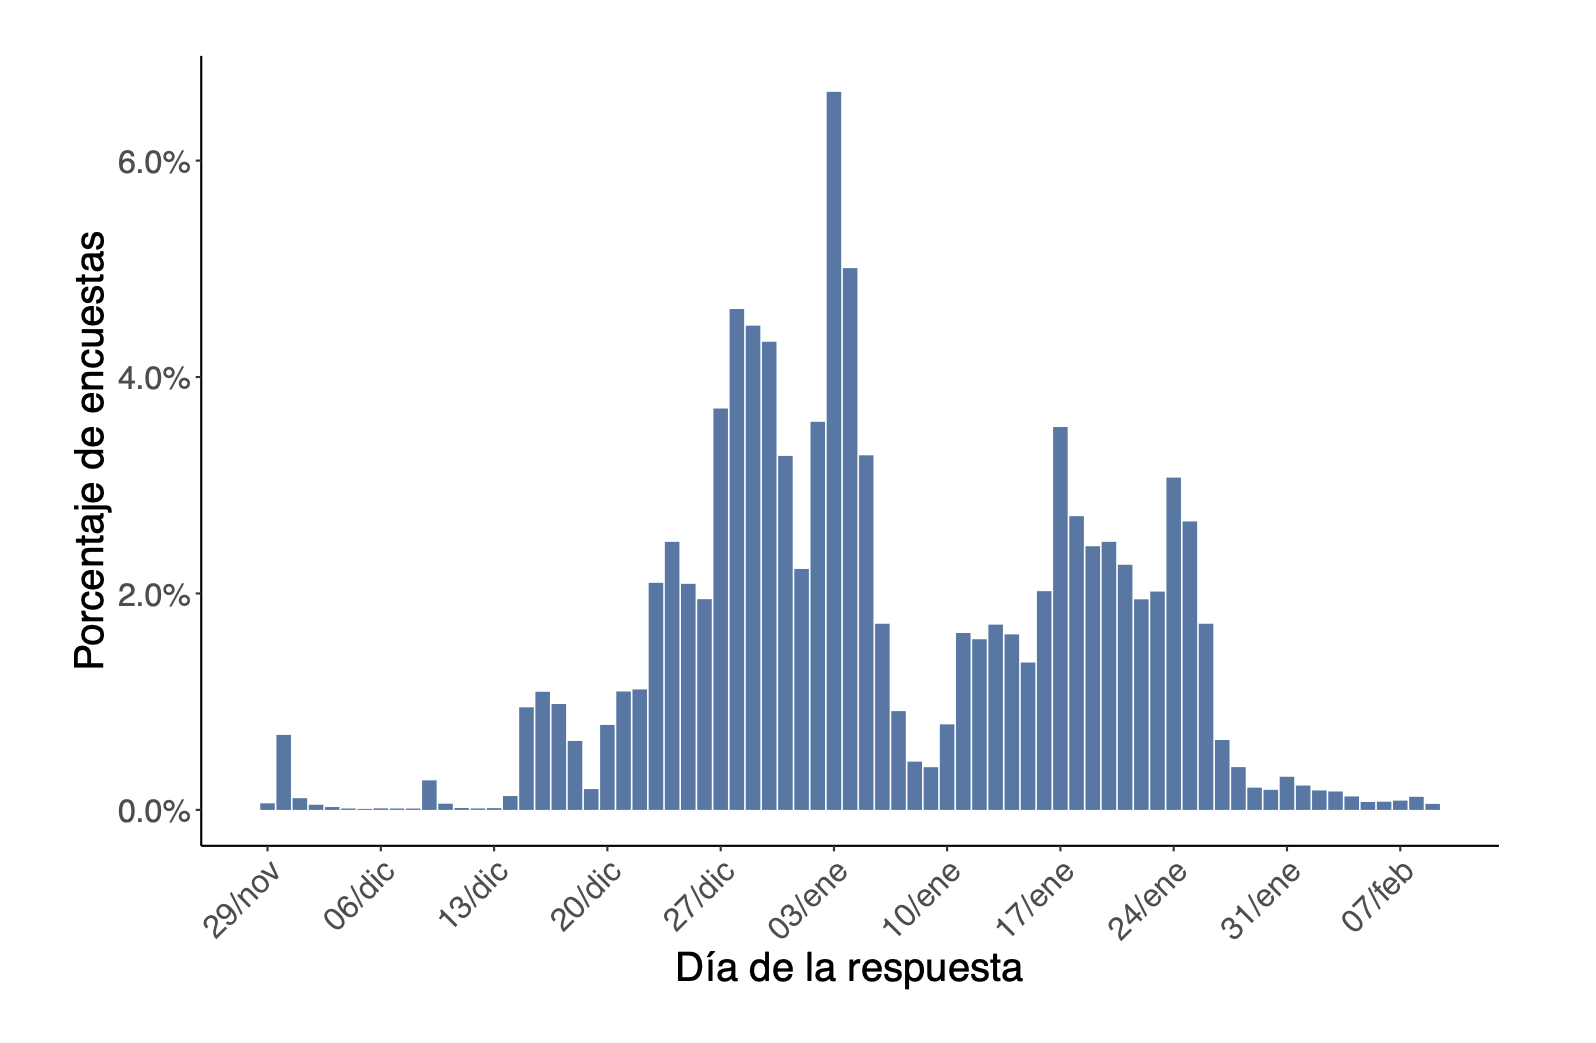
\includegraphics[width=\textwidth]{04_Figures/workey_survey/Exp_1.png}
    \end{subfigure}
    \begin{subfigure}{0.49\textwidth}
    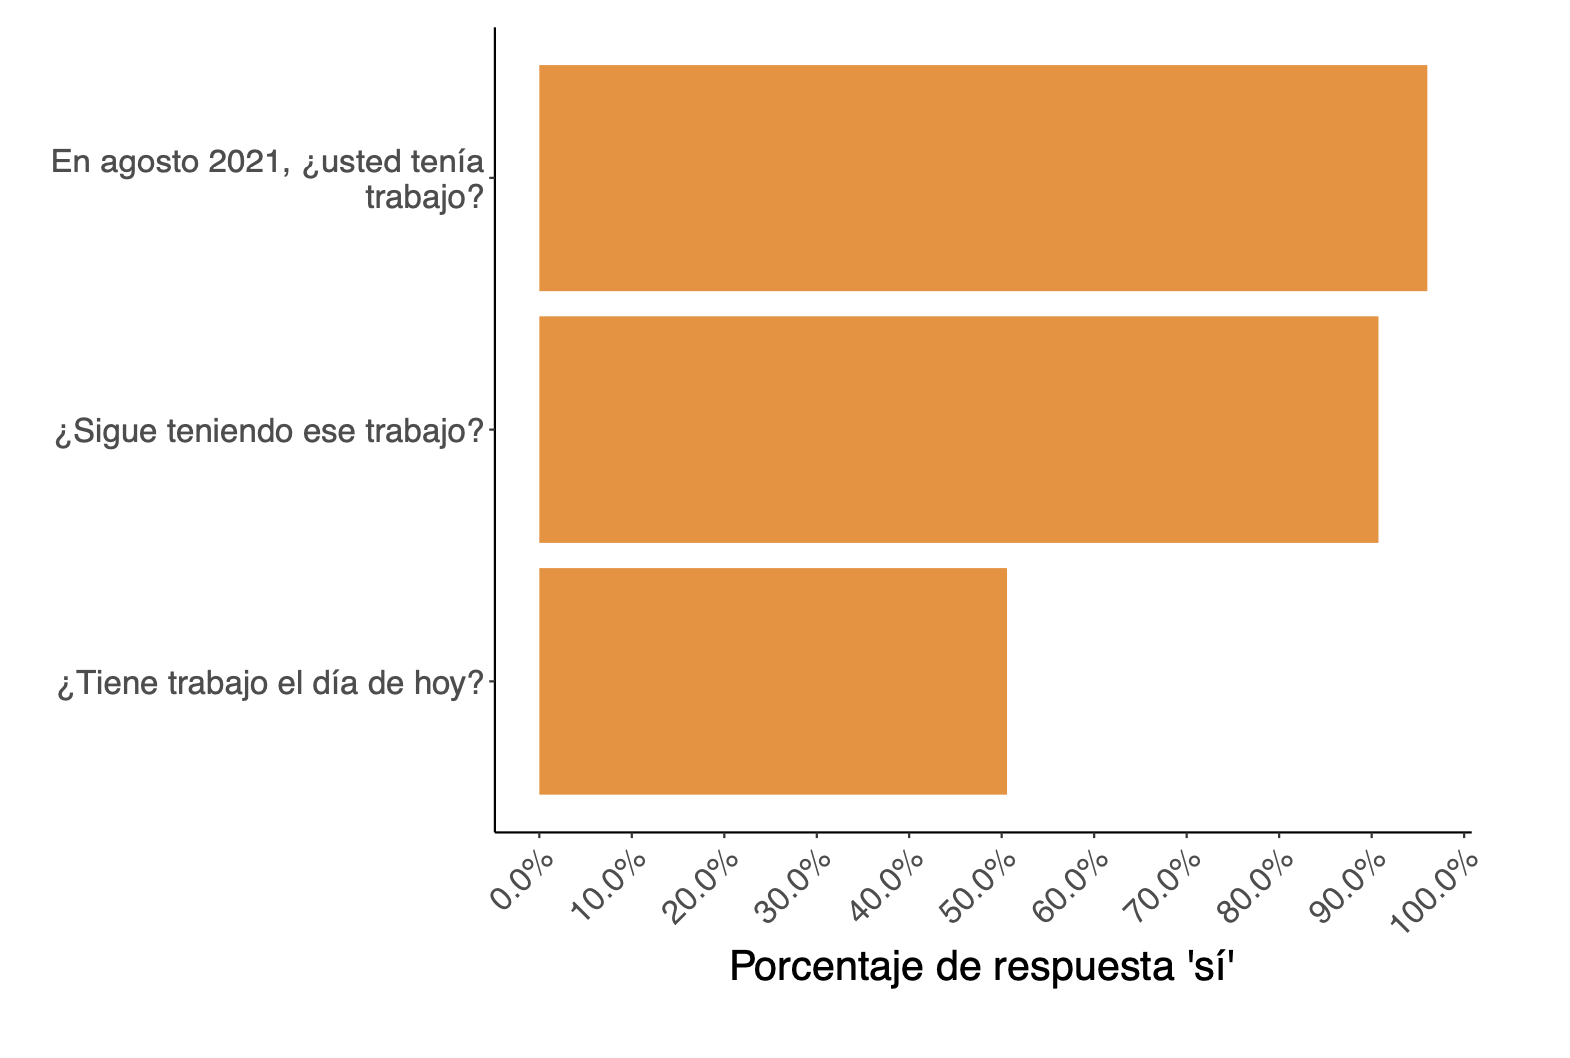
\includegraphics[width=\textwidth]{04_Figures/workey_survey/Exp_2.png}
    \end{subfigure}
    
    \begin{subfigure}{0.49\textwidth}
    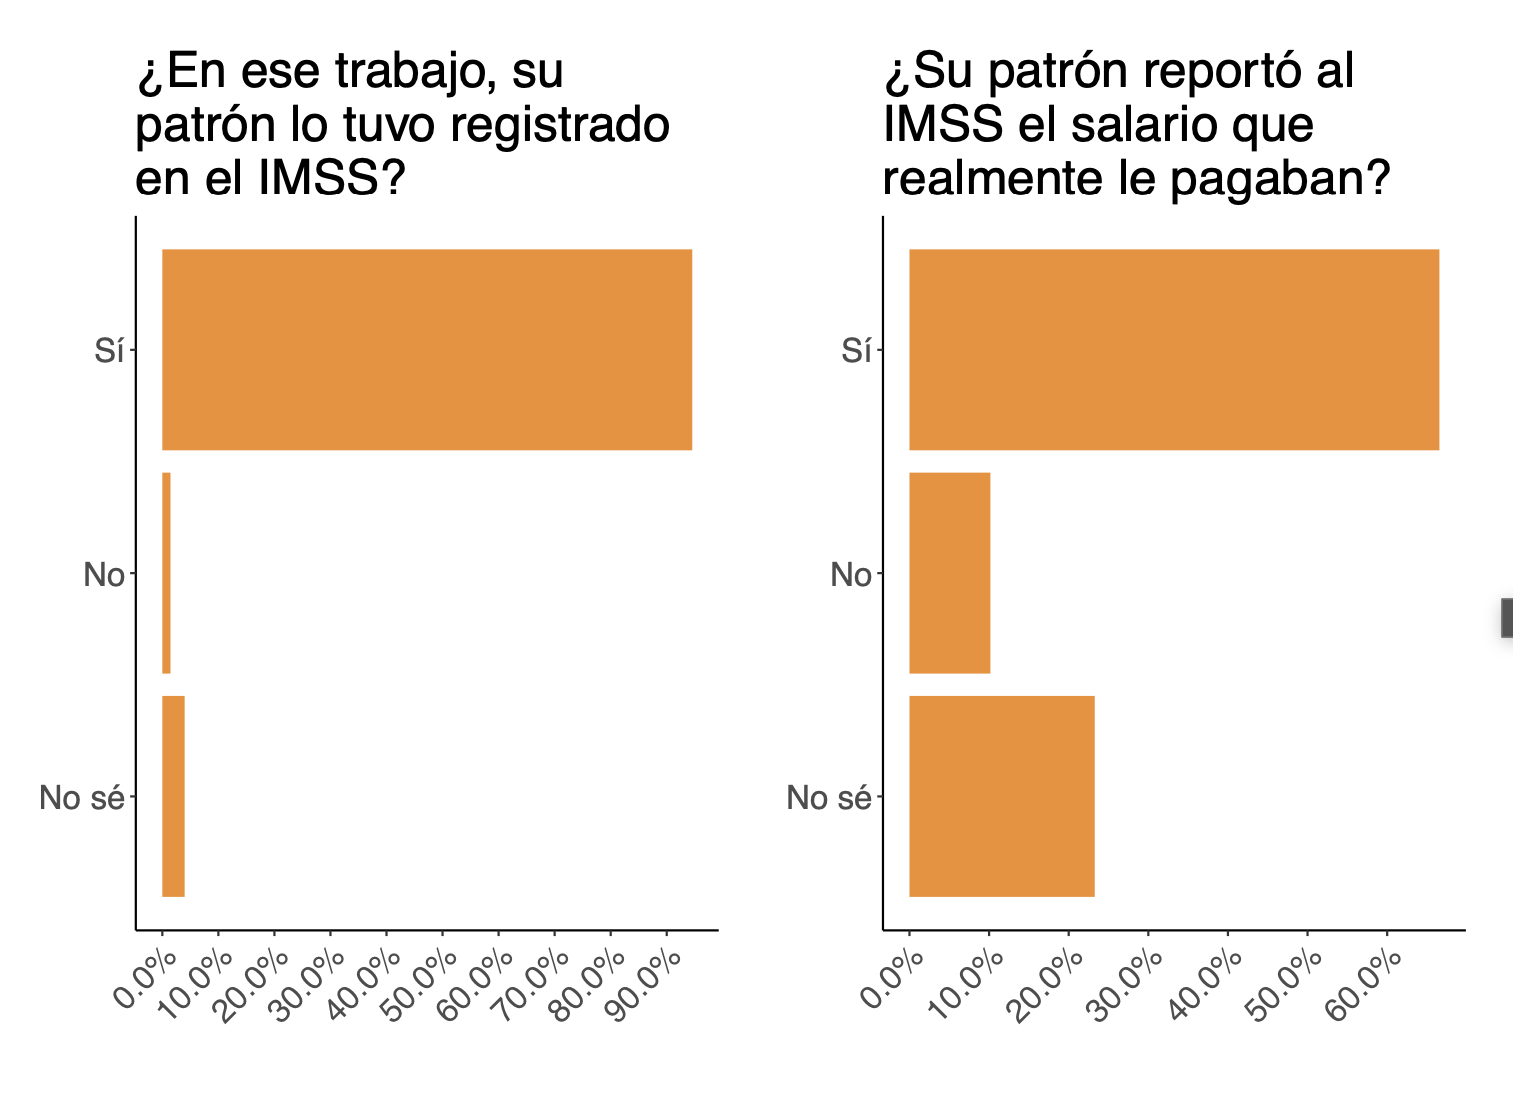
\includegraphics[width=\textwidth]{04_Figures/workey_survey/Exp_3.png}
    \end{subfigure}
    \begin{subfigure}{0.49\textwidth}
    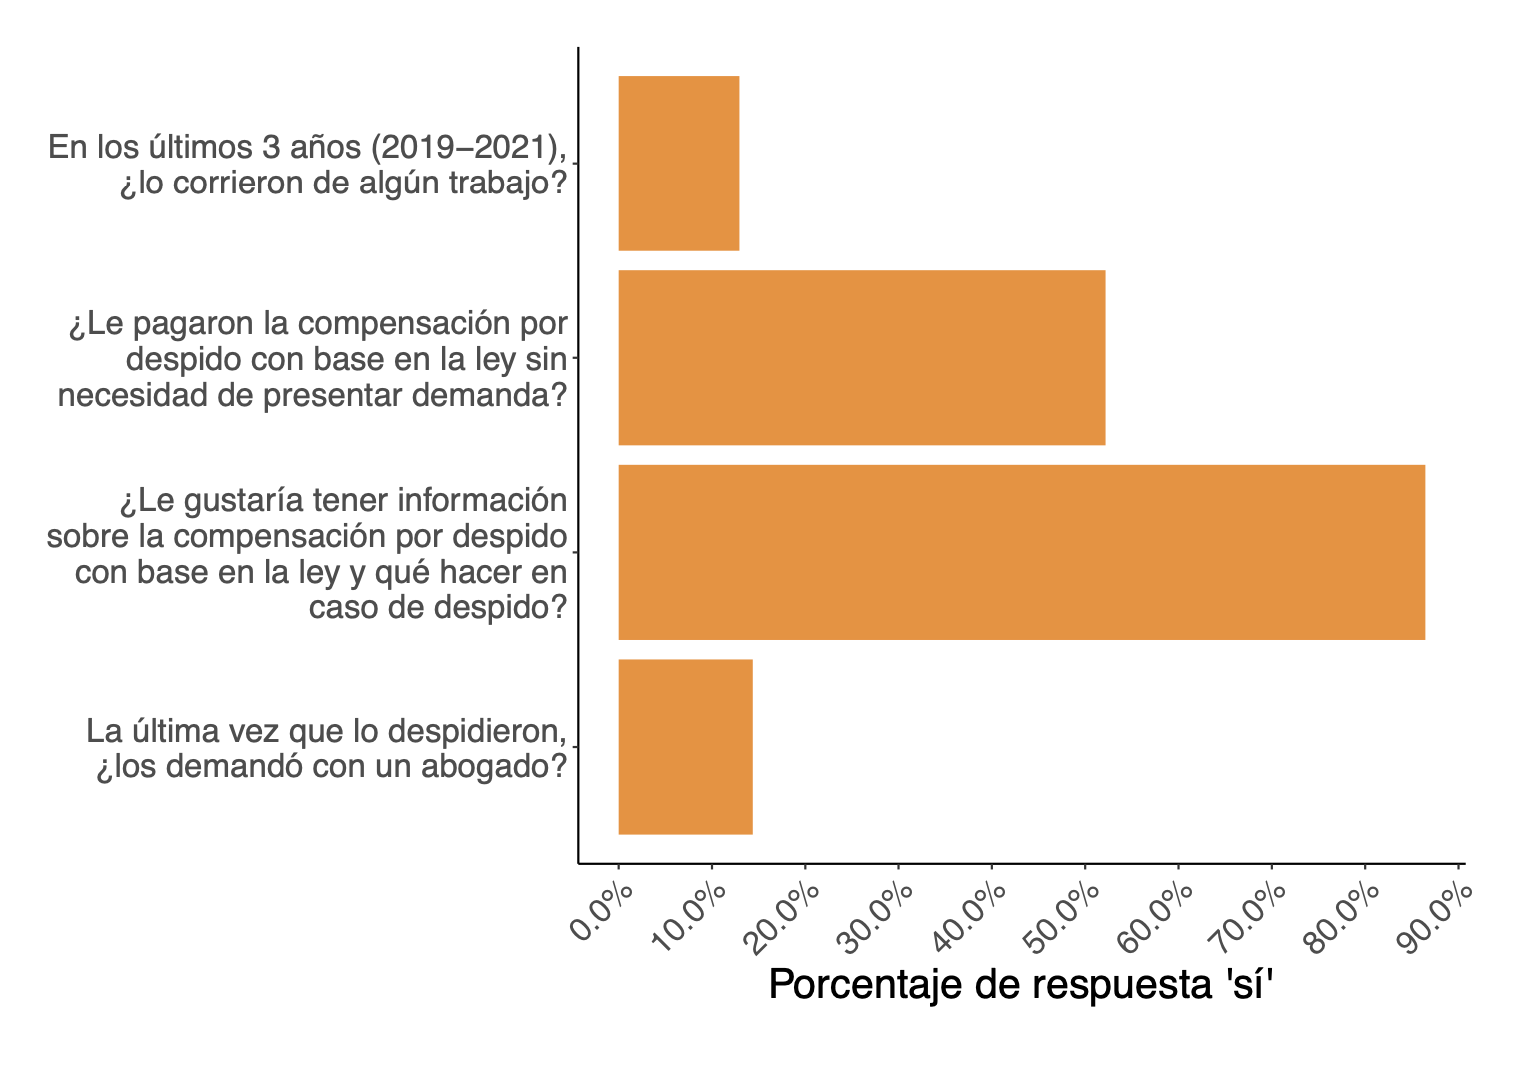
\includegraphics[width=\textwidth]{04_Figures/workey_survey/Exp_4.png}
    \end{subfigure}
    
    \begin{subfigure}{0.49\textwidth}
    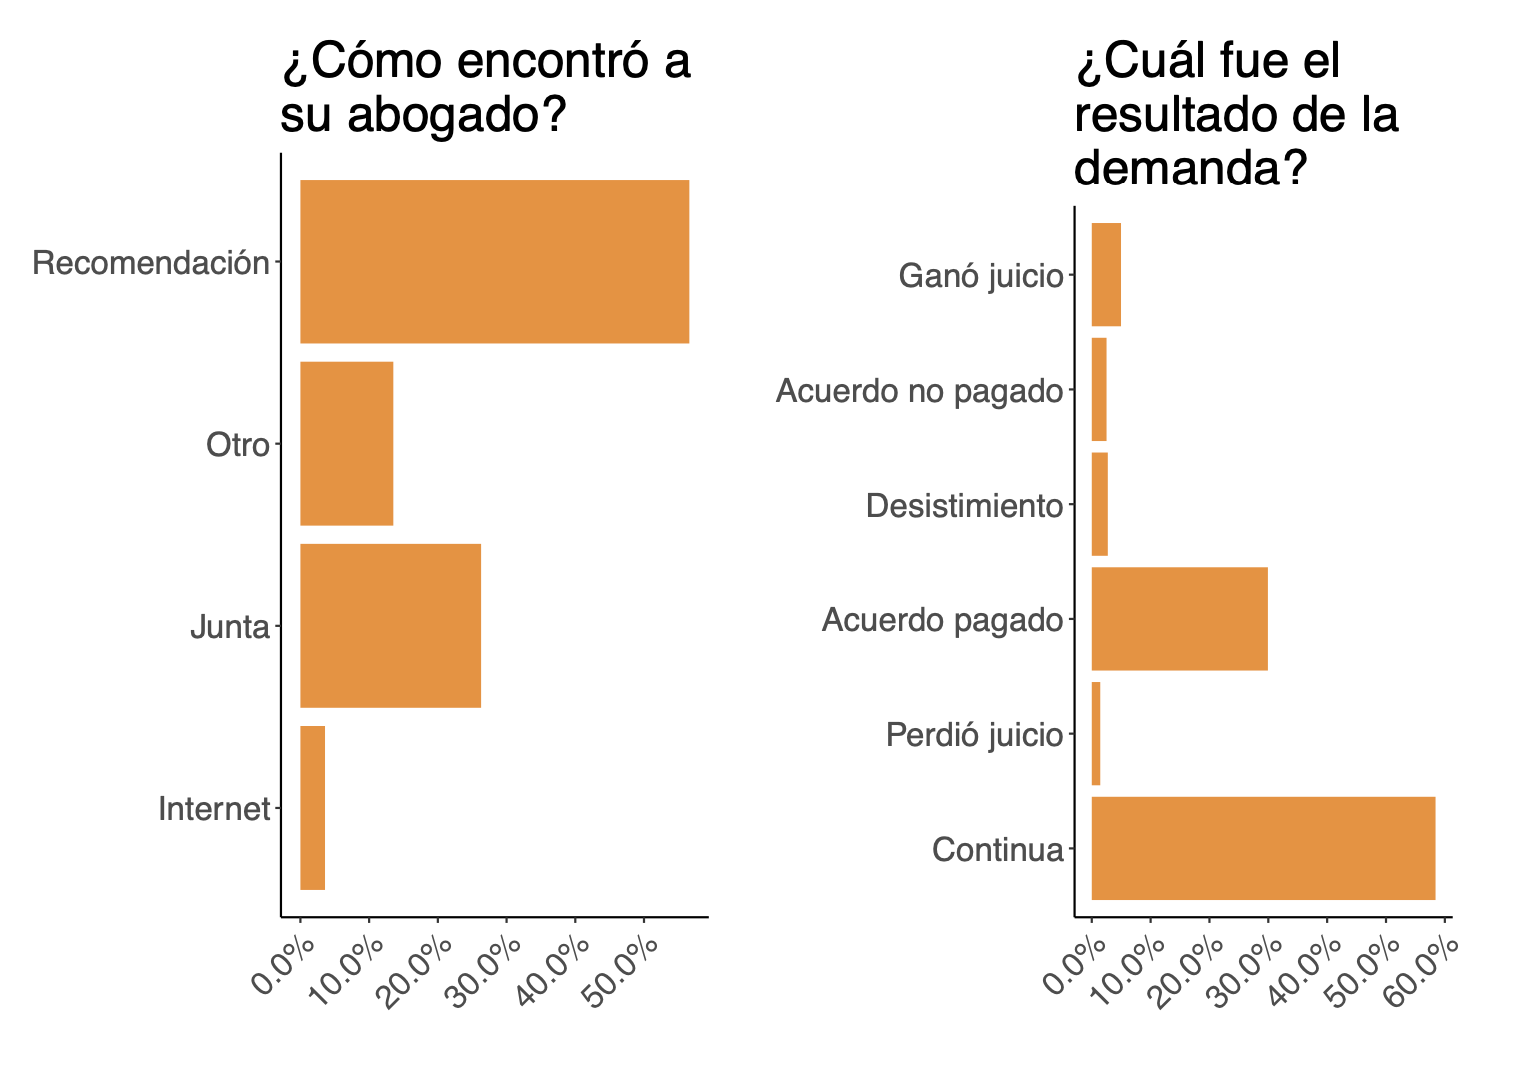
\includegraphics[width=\textwidth]{04_Figures/workey_survey/Exp_5.png}
    \end{subfigure}
    \begin{subfigure}{0.49\textwidth}
    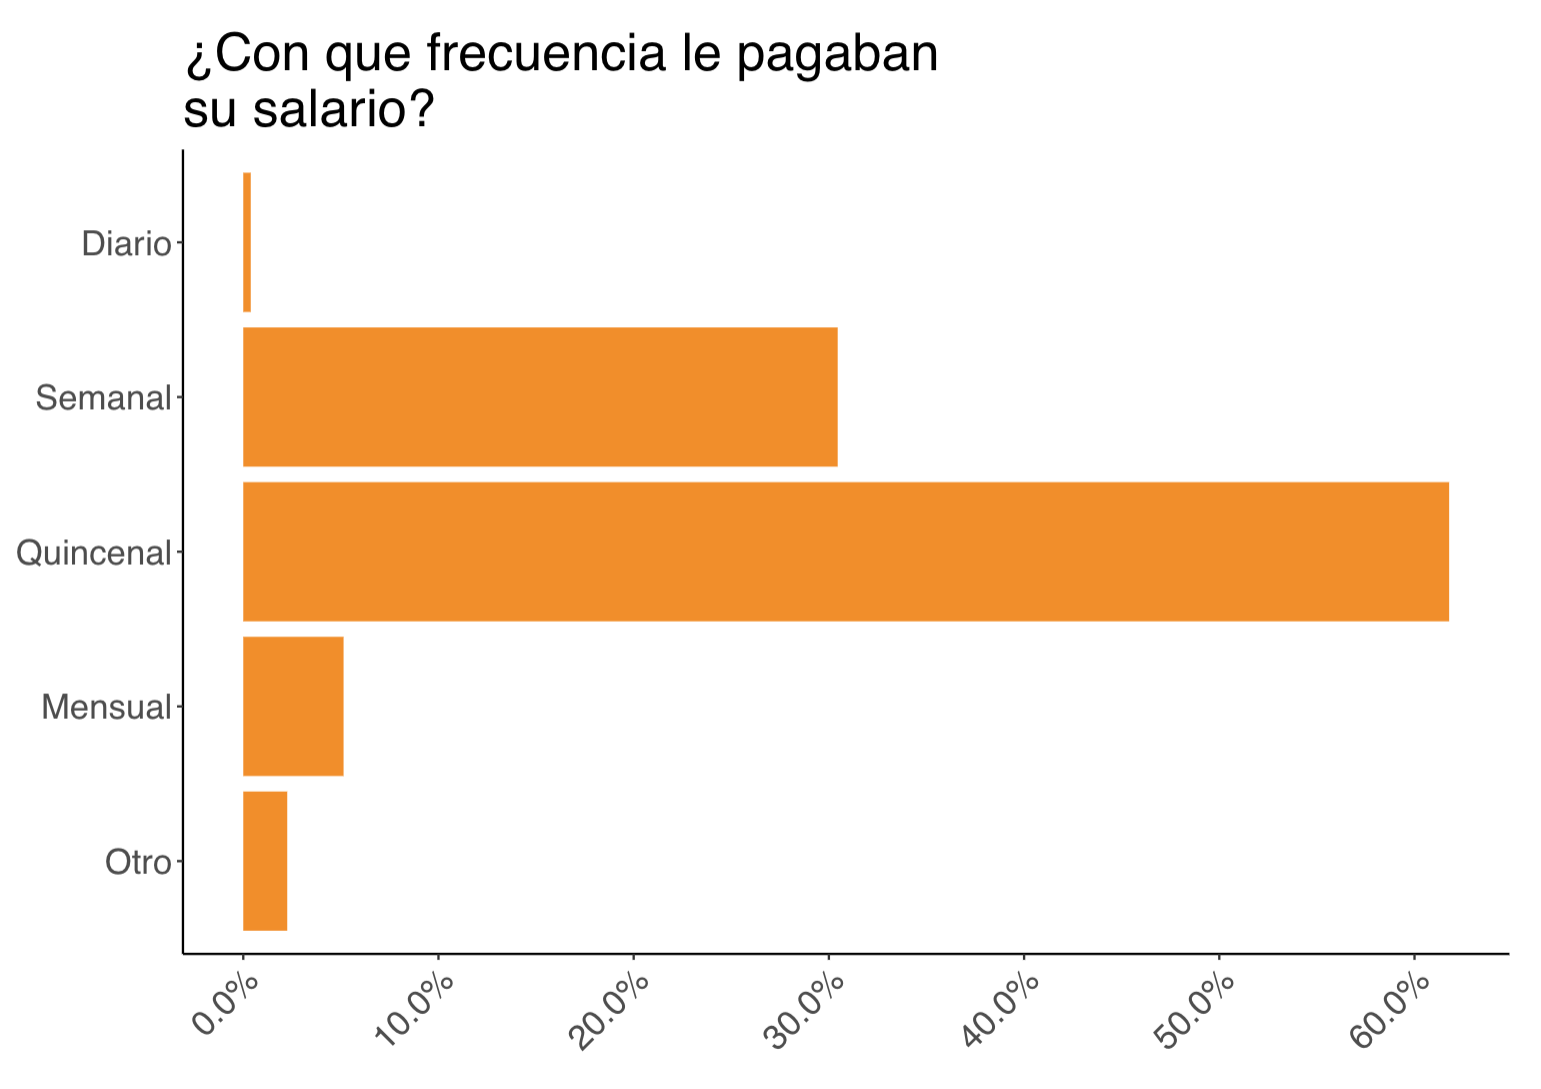
\includegraphics[width=\textwidth]{04_Figures/workey_survey/Exp_6.png}
    \end{subfigure}
    
    \end{center}
\end{figure}

\clearpage

\begin{figure}[H]
    \caption{Worker Survey Graphs}
    \label{worker_surver_2}
    \begin{center}

    \begin{subfigure}{0.49\textwidth}
    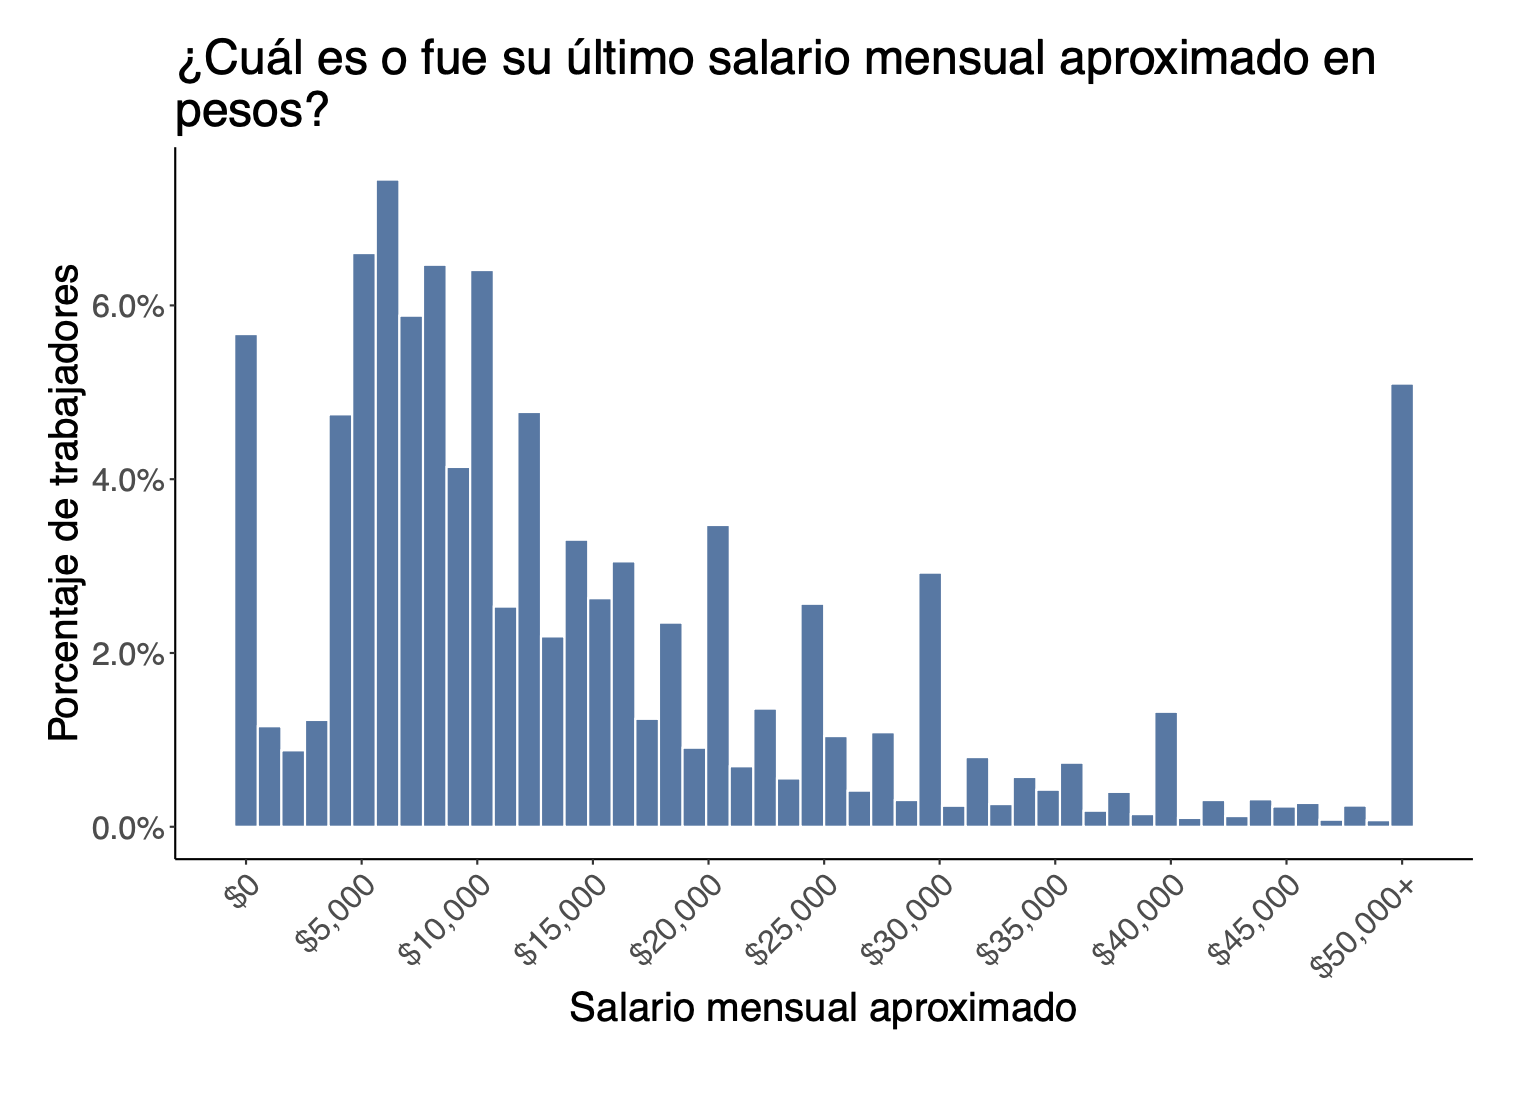
\includegraphics[width=\textwidth]{04_Figures/workey_survey/Exp_7.png}
    \end{subfigure}
    \begin{subfigure}{0.49\textwidth}
    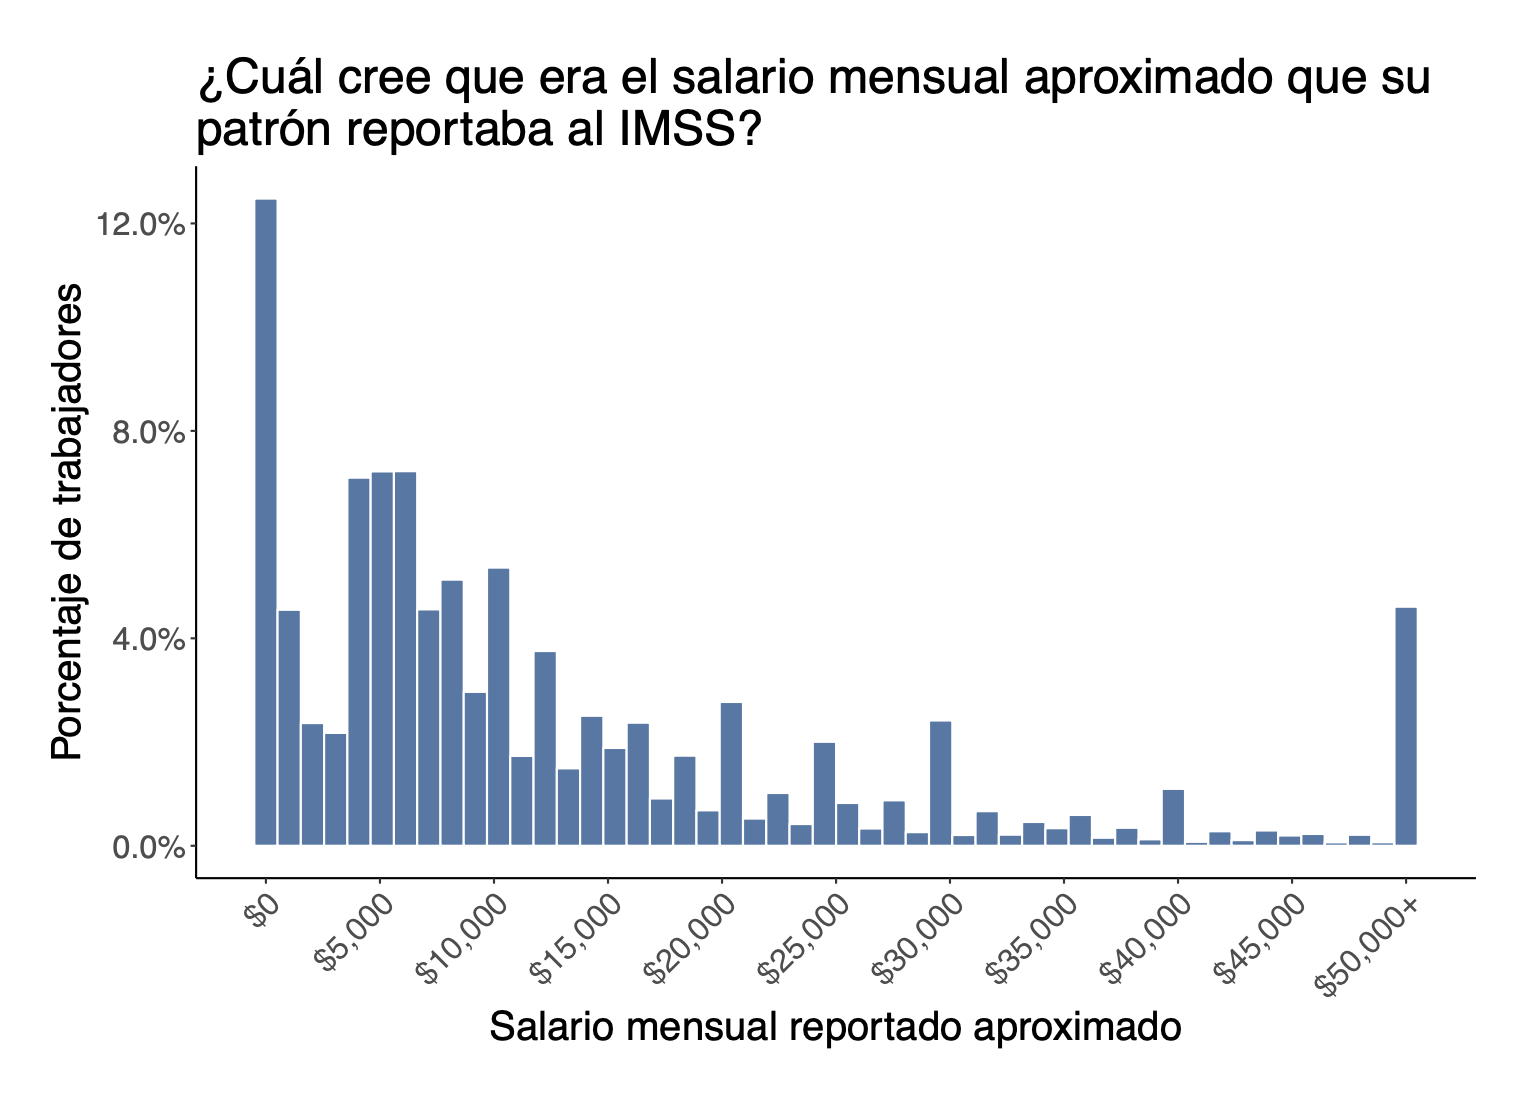
\includegraphics[width=\textwidth]{04_Figures/workey_survey/Exp_8.png}
    \end{subfigure}
    
    \begin{subfigure}{0.49\textwidth}
    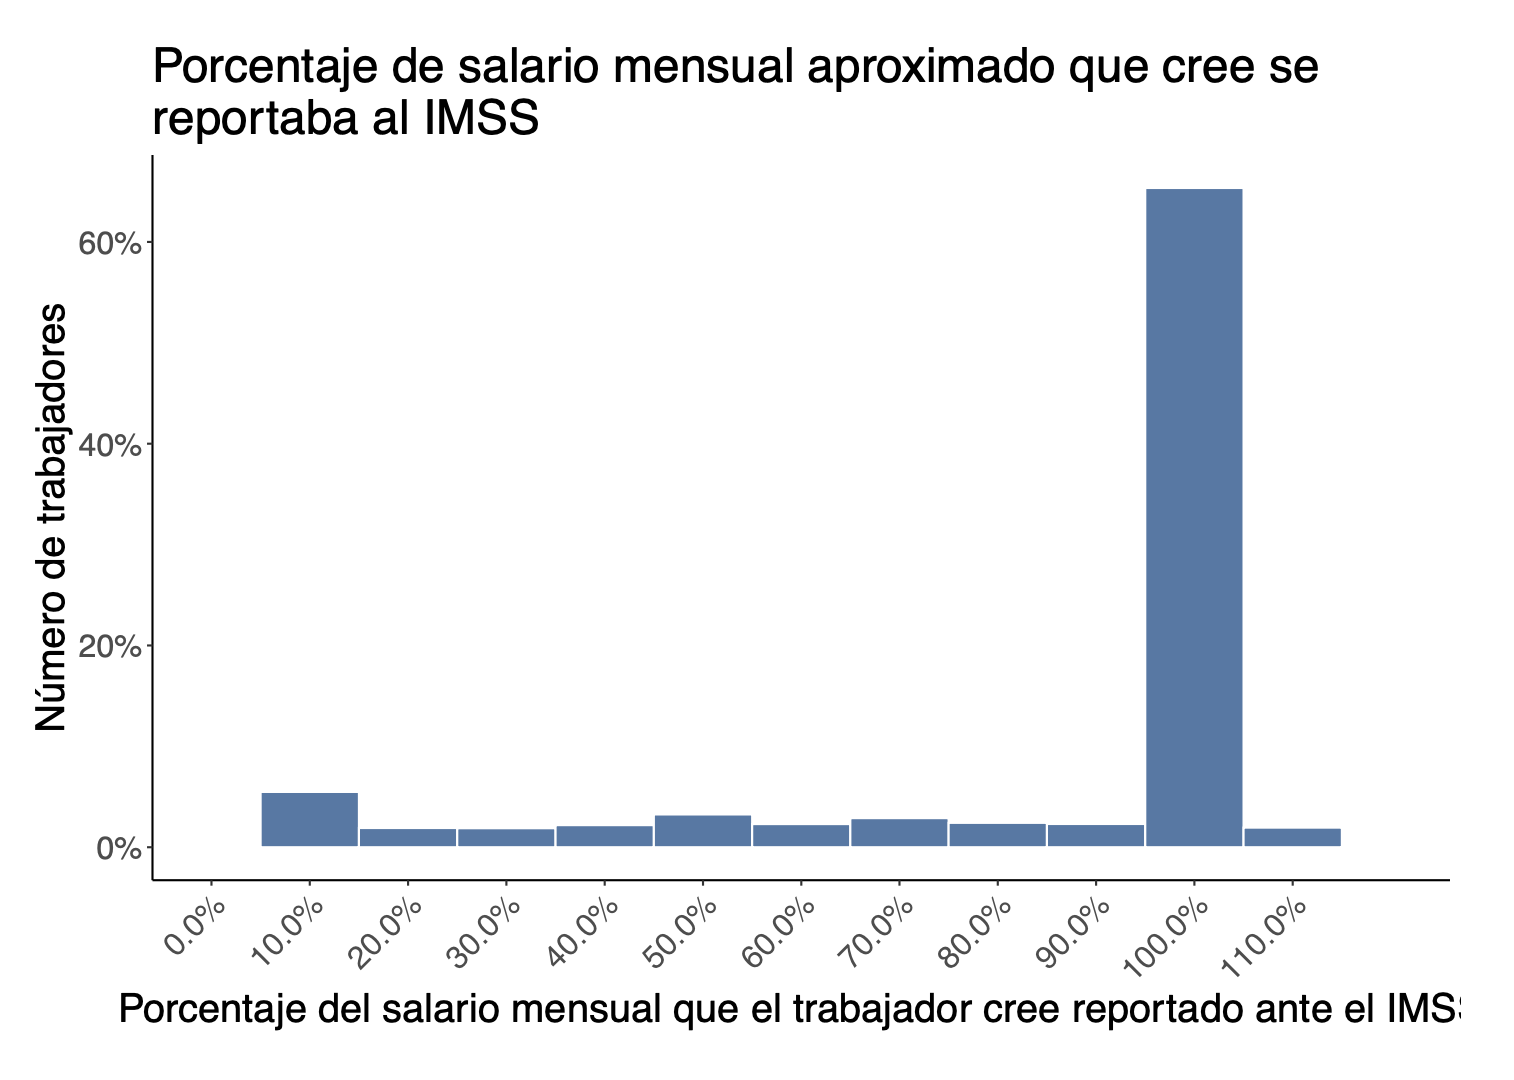
\includegraphics[width=\textwidth]{04_Figures/workey_survey/Exp_9.png}
    \end{subfigure}
    \begin{subfigure}{0.49\textwidth}
    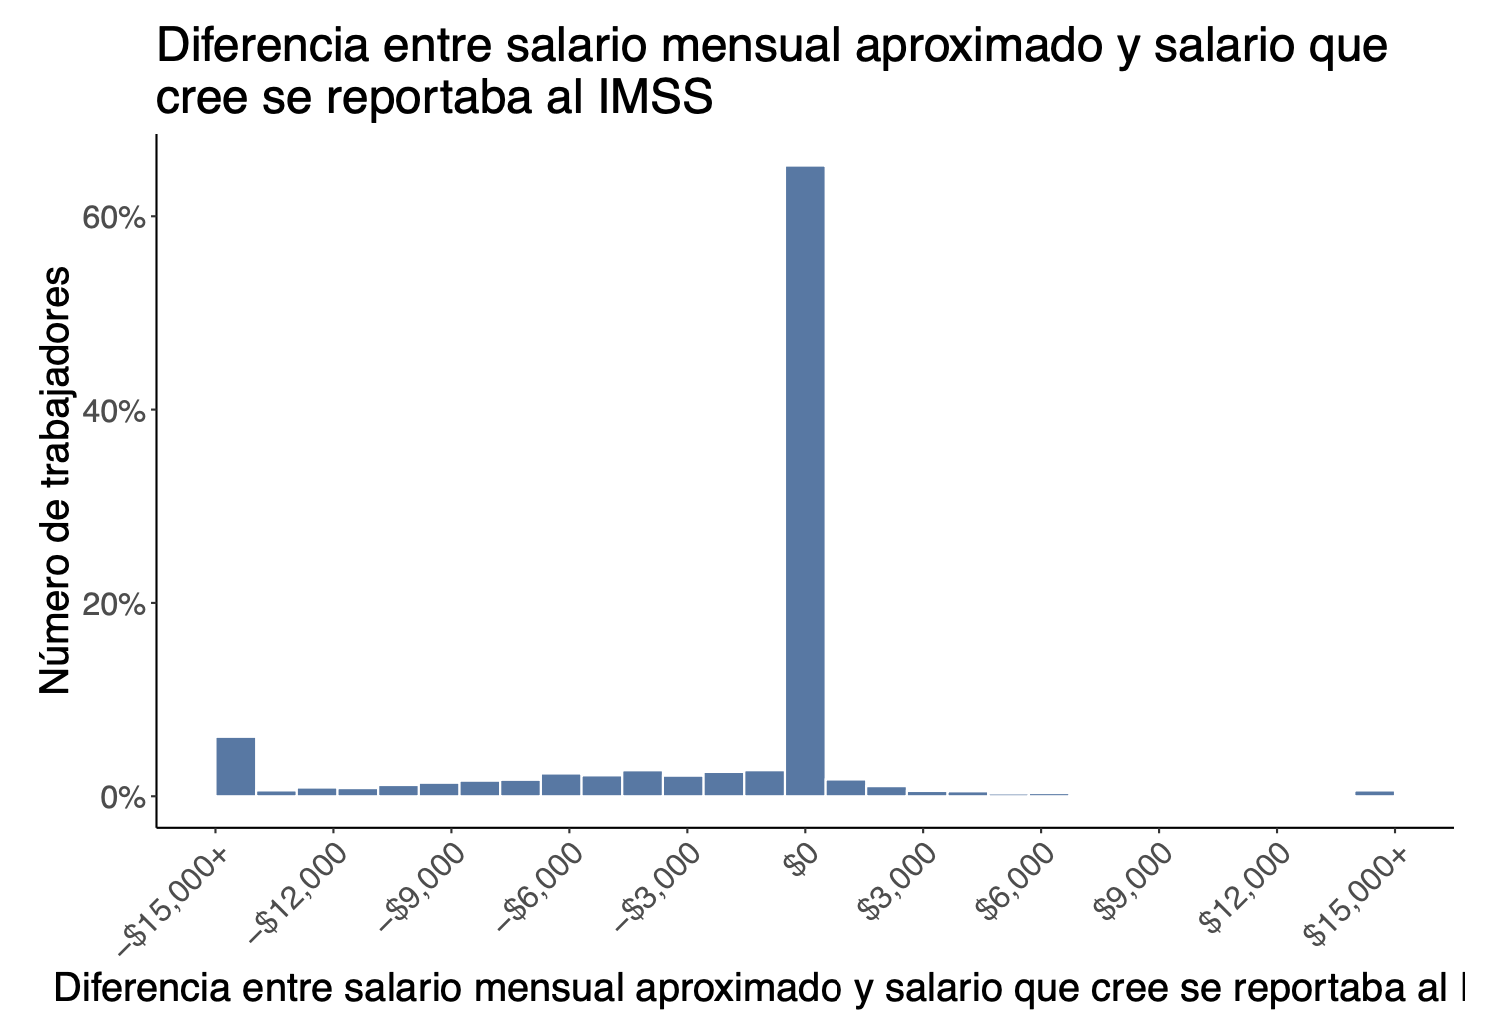
\includegraphics[width=\textwidth]{04_Figures/workey_survey/Exp_10.png}
    \end{subfigure}
    
    \begin{subfigure}{0.49\textwidth}
    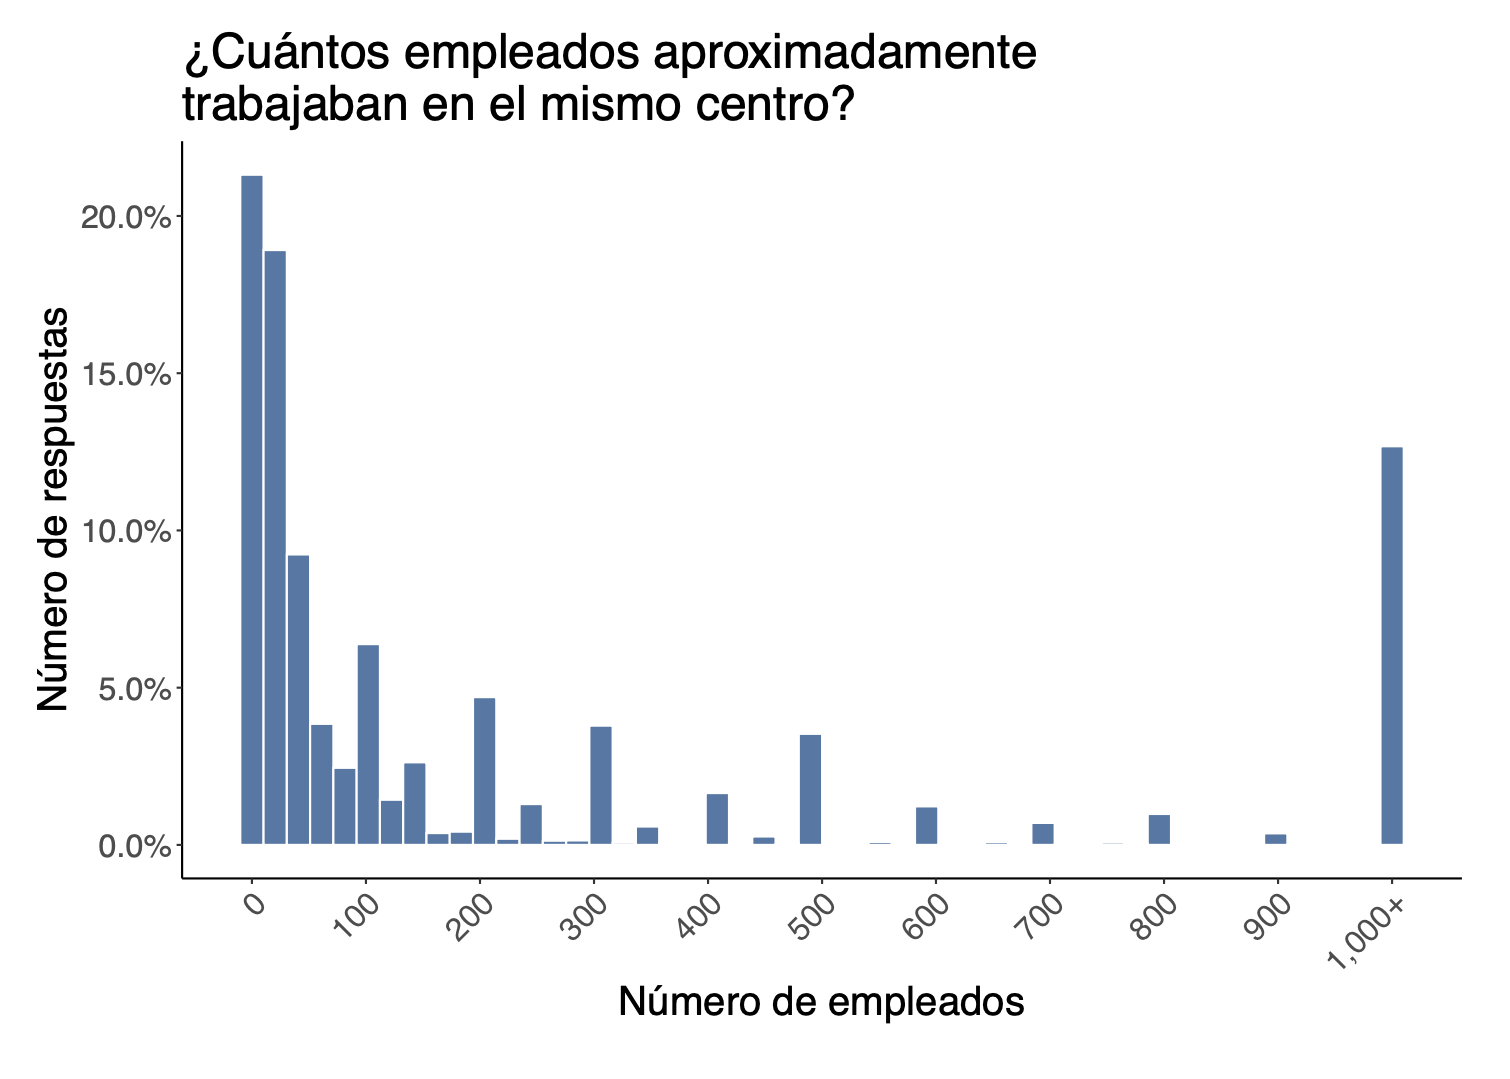
\includegraphics[width=\textwidth]{04_Figures/workey_survey/Exp_11.png}
    \end{subfigure}
    \begin{subfigure}{0.49\textwidth}
    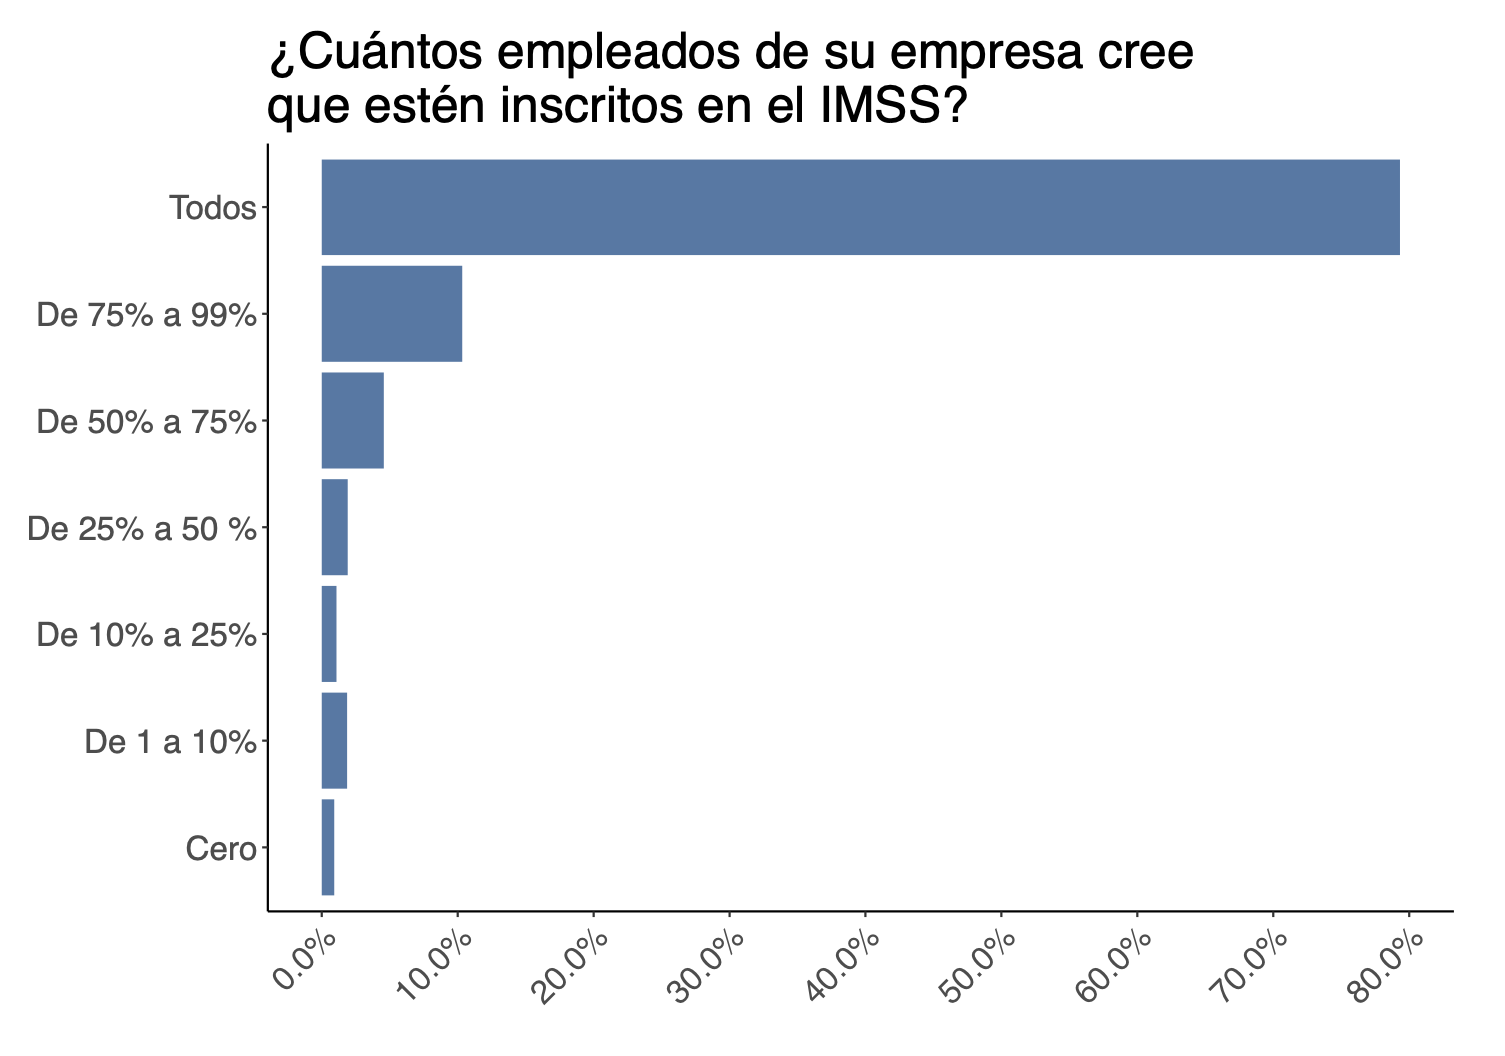
\includegraphics[width=\textwidth]{04_Figures/workey_survey/Exp_12.png}
    \end{subfigure}
    
    \end{center}
\end{figure}

\clearpage

\begin{figure}[H]
    \caption{Worker Survey Graphs}
    \label{worker_surver_3}
    \begin{center}

    \begin{subfigure}{0.49\textwidth}
    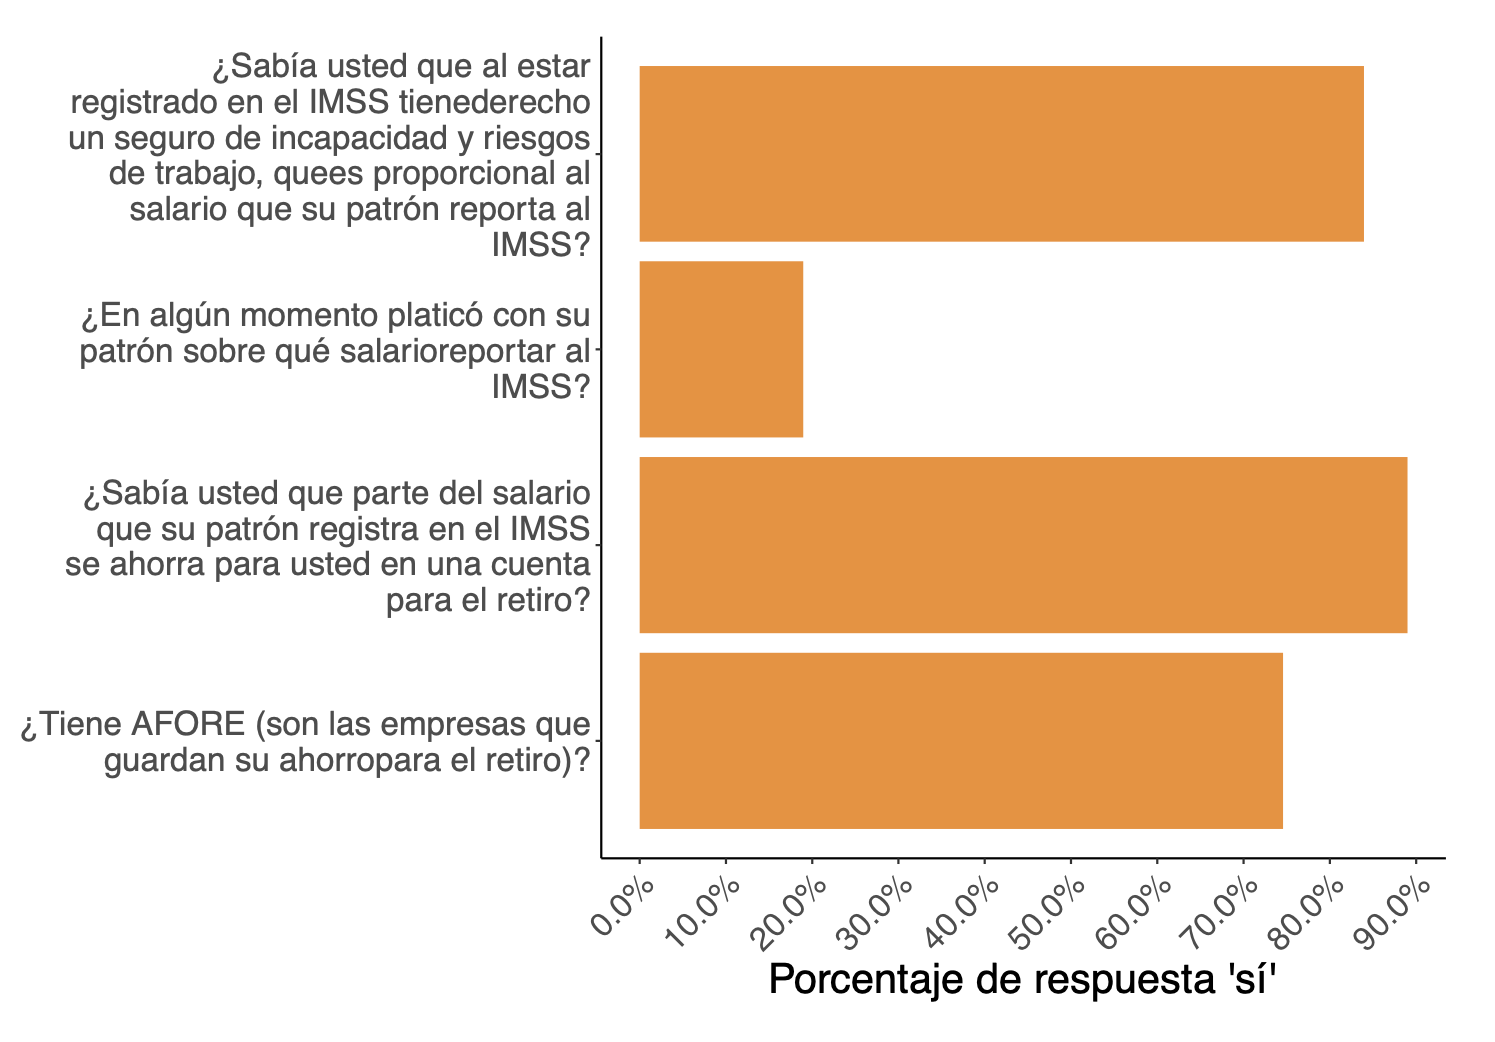
\includegraphics[width=\textwidth]{04_Figures/workey_survey/Exp_13.png}
    \end{subfigure}
    \begin{subfigure}{0.49\textwidth}
    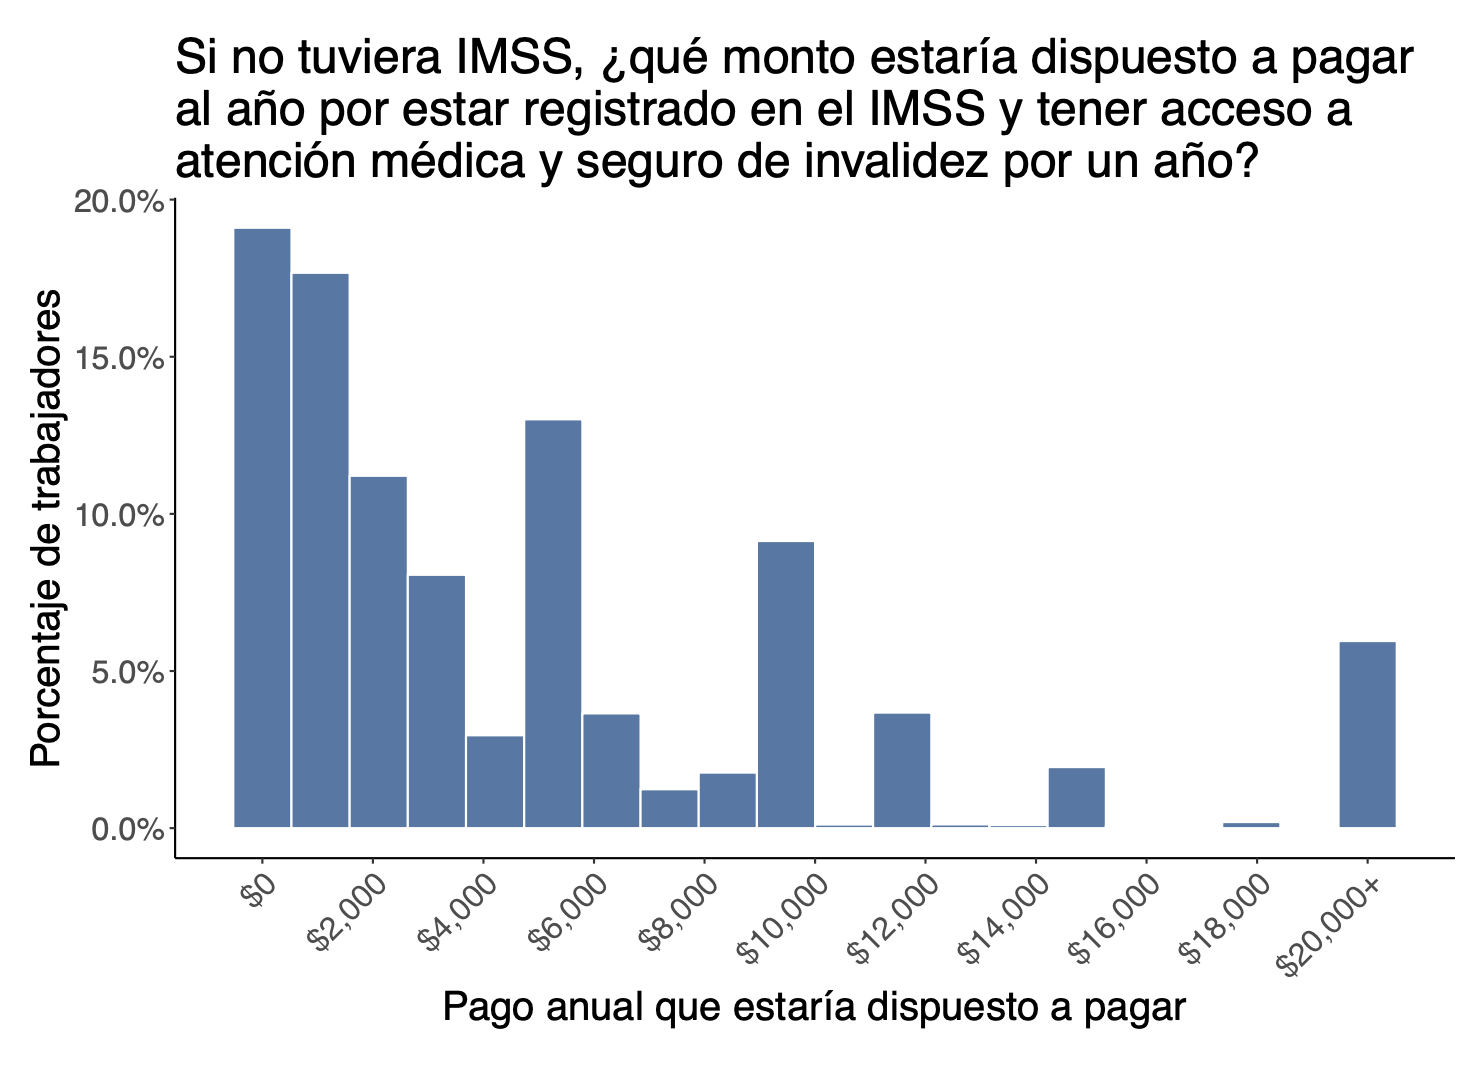
\includegraphics[width=\textwidth]{04_Figures/workey_survey/Exp_14.png}
    \end{subfigure}
    
    \begin{subfigure}{0.49\textwidth}
    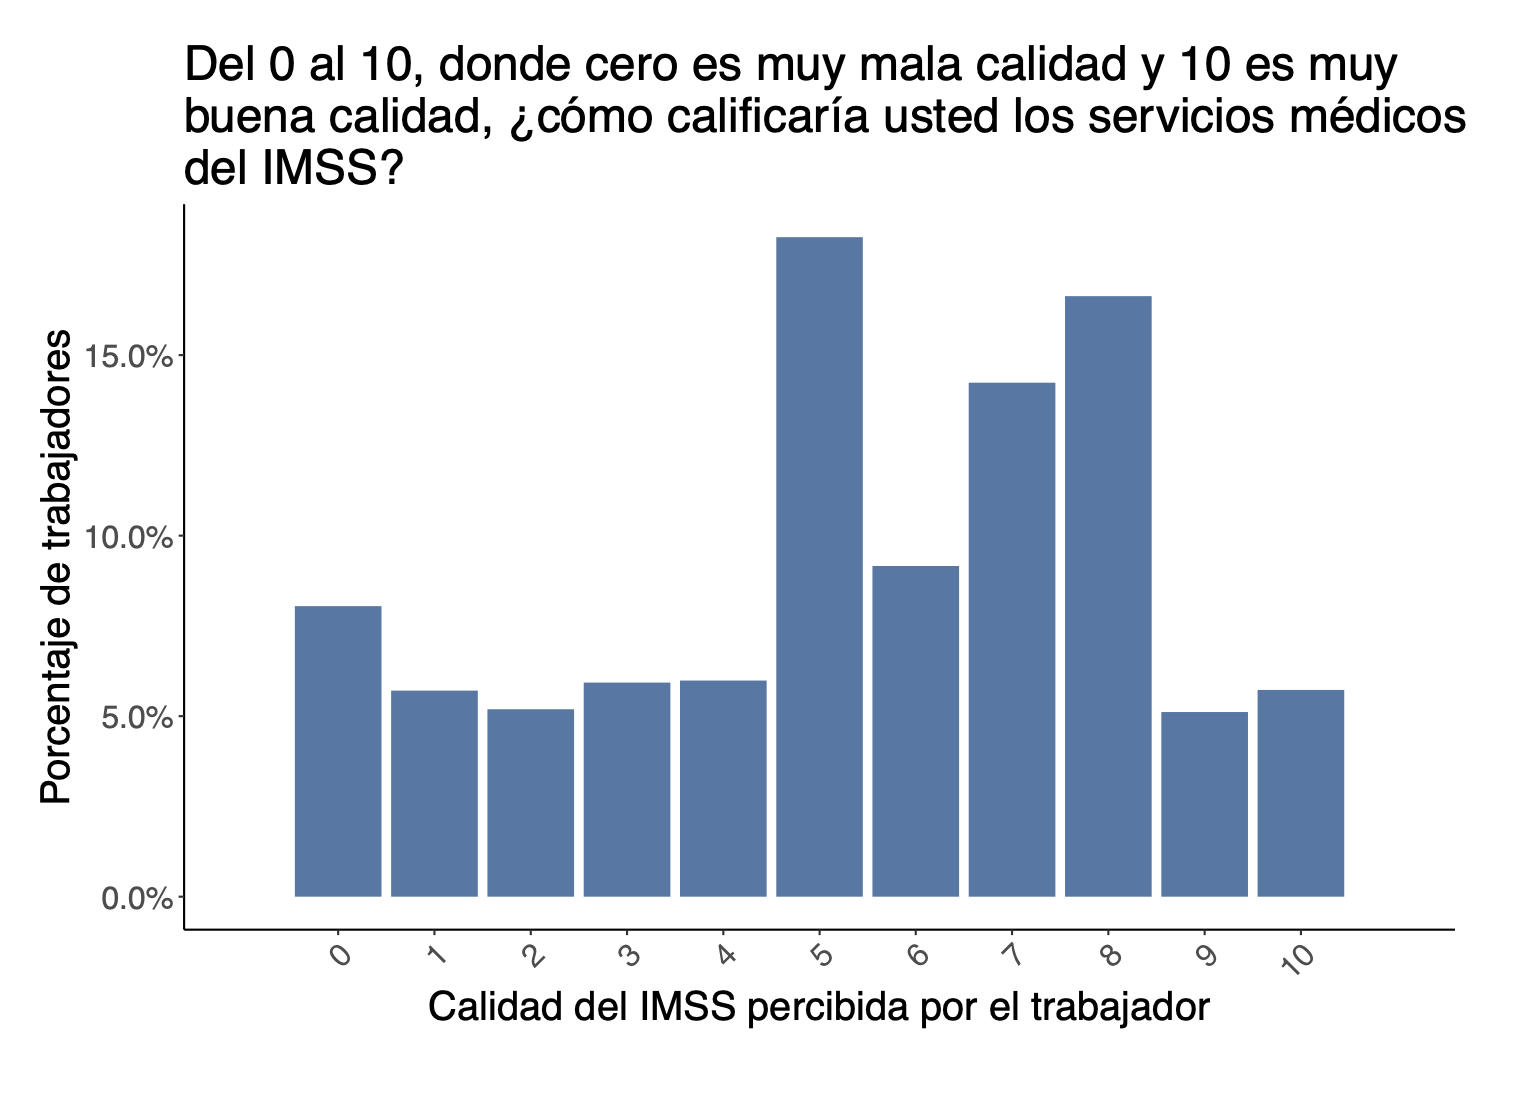
\includegraphics[width=\textwidth]{04_Figures/workey_survey/Exp_15.png}
    \end{subfigure}
    \begin{subfigure}{0.49\textwidth}
    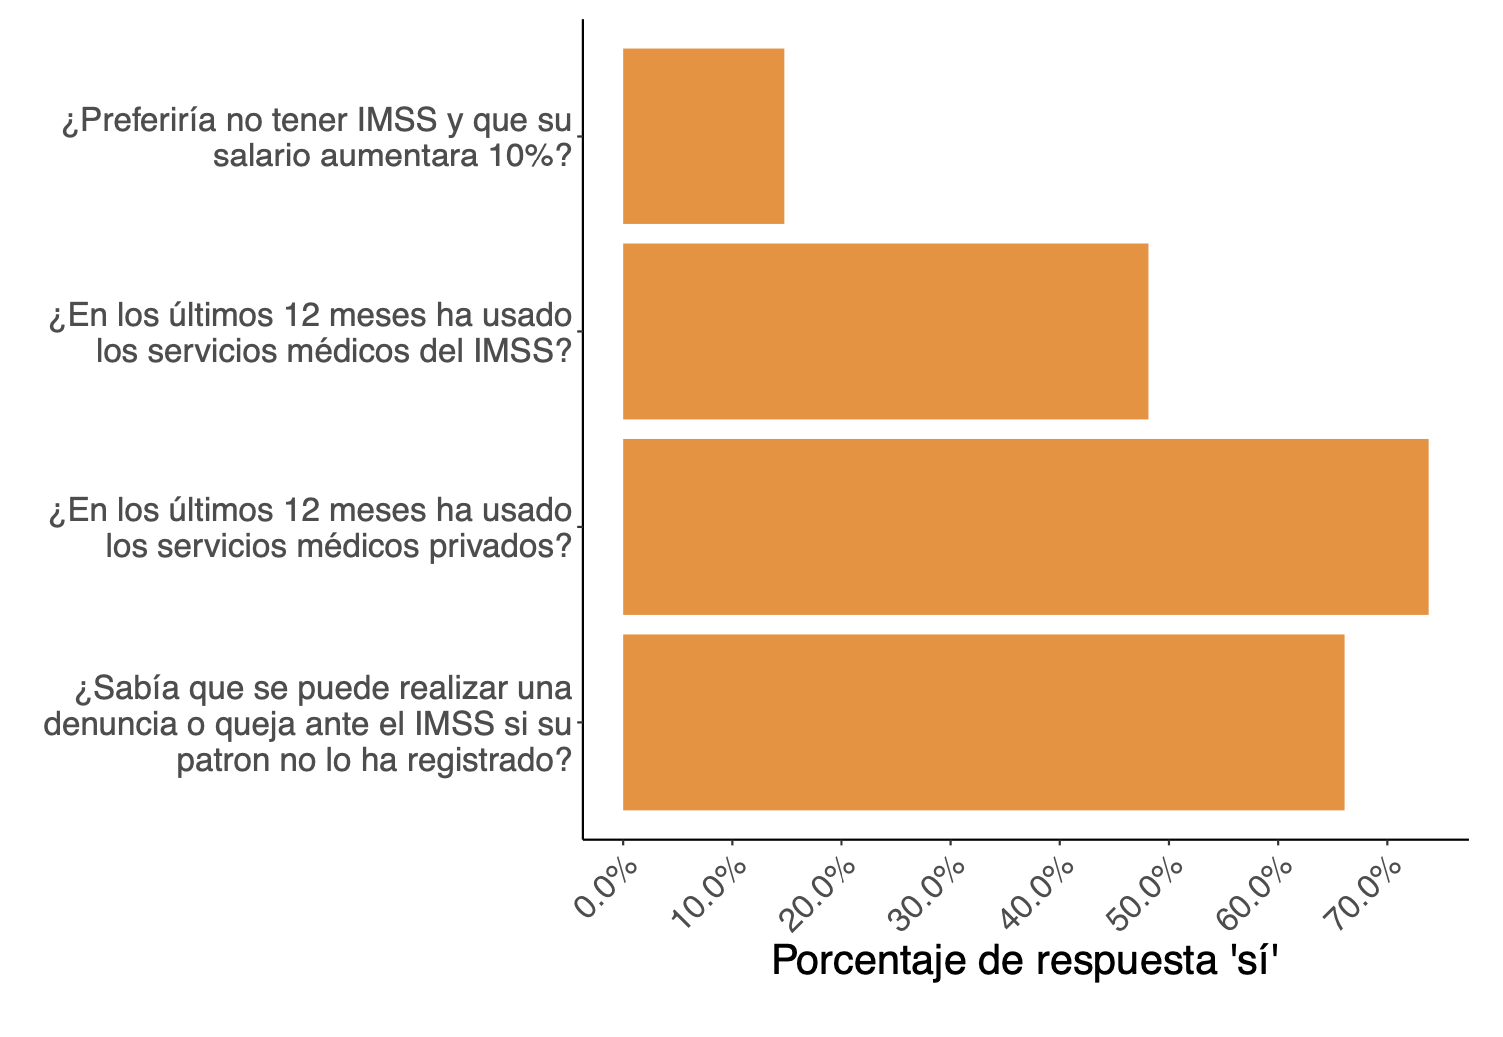
\includegraphics[width=\textwidth]{04_Figures/workey_survey/Exp_16.png}
    \end{subfigure}
    
    \end{center}
\end{figure}


%%%%%%%%%%%%%%%%%%%%%%%%%%%%%%%%%%%%%%%%%%%%%%%%%%%%%%

\newpage
%  \documentclass[oneside,11pt]{article}

% 
\usepackage{soul}
\usepackage{natbib}
\usepackage{hyperref}
\usepackage{bookmark}
\usepackage{graphicx}             
\graphicspath{{./Figuras/}}
\usepackage[dvipsnames]{xcolor}
\usepackage{todonotes}
\usepackage{makecell}
\usepackage[margin=1in]{geometry}
\usepackage{float}                
\usepackage{amsmath}
\usepackage{amscd}
\usepackage{amsfonts}
\usepackage{amssymb}
\usepackage{bbm}
\usepackage{booktabs}
\usepackage{nameref}
\usepackage{multirow}
\usepackage[nokeyprefix]{refstyle}
\usepackage{rotating}
\usepackage{threeparttable}
\usepackage{afterpage}
\usepackage{lscape}
\usepackage{enumerate}
\usepackage{caption}
\usepackage{subcaption}
\usepackage{epstopdf}
\usepackage{setspace}
\usepackage{svg}
\usepackage{dsfont}
\usepackage{amsthm}
\usepackage{tocloft}
\usepackage{etoc}
\usepackage{lmodern}
\usepackage{bm}
\usepackage[T1]{fontenc}
\usepackage{tgpagella}

\epstopdfDeclareGraphicsRule{.tiff}{png}{.png}{convert #1 \OutputFile}
\AppendGraphicsExtensions{.tiff}

\epstopdfDeclareGraphicsRule{.tif}{png}{.png}{convert #1 \OutputFile}
\AppendGraphicsExtensions{.tif}

\def\sym#1{\ifmmode^{#1}\else\(^{#1}\)\fi}

\usepackage{tikz}
\usetikzlibrary{shapes.geometric, arrows}
\usetikzlibrary{calc}
\usetikzlibrary{matrix}

\tikzset{ 
    table/.style={
        matrix of nodes,
        row sep=-\pgflinewidth,
        column sep=-\pgflinewidth,
        nodes={
            rectangle,
            draw=black,
            align=center
        },
        minimum height=1.5em,
        text depth=0.5ex,
        text height=2ex,
        nodes in empty cells,
%%
        every even row/.style={
            nodes={fill=gray!20}
        },
        column 1/.style={
            nodes={text width=2em,font=\bfseries}
        },
        row 1/.style={
            nodes={
                fill=black,
                text=white,
                font=\bfseries
            }
        }
    }
}


\usepackage{colortbl}
\usepackage{url}
\urlstyle{rm}
\definecolor{darkblue}{rgb}{0,0,.4}
\hypersetup{colorlinks=true, breaklinks=true, citecolor=Maroon, linkcolor=darkblue, menucolor=darkblue, urlcolor=darkblue}

\newtheorem{theorem}{Theorem}
\newtheorem{claim}[theorem]{Claim}
\newtheorem{prop}[theorem]{Proposition} 
\newtheorem{cor}[theorem]{Corollary} 
\newtheorem{assumption}{Assumption} 
\newtheorem{lem}{Lemma} 

\DeclareRobustCommand{\hlgr}[1]{{\sethlcolor{green}\hl{#1}}}


\usepackage{comment}
%para esconder columnas en tablas (enrique)
\usepackage{array}
\newcolumntype{H}{>{\setbox0=\hbox\bgroup}c<{\egroup}@{}}
\linespread{1.25}

\newcommand{\wh}{\widehat}
\usepackage{anyfontsize}

\usepackage[linesnumbered,vlined,ruled,commentsnumbered]{algorithm2e}

\DontPrintSemicolon
\newcommand{\To}{\mbox{\upshape\bfseries to}}
\newcommand{\E}{\mathbb{E}}

\DeclareCaptionFormat{cont}{#1 (cont.)#2#3\par}
% %%% HELPER CODE FOR DEALING WITH EXTERNAL REFERENCES
% \usepackage{xr}
% \makeatletter
% \newcommand*{\addFileDependency}[1]{
%   \typeout{(#1)}
%   \@addtofilelist{#1}
%   \IfFileExists{#1}{}{\typeout{No file #1.}}
% }
% \makeatother


% \newcommand*{\myexternaldocument}[1]{
%     \externaldocument{#1}
%     \addFileDependency{#1.tex}
%     \addFileDependency{#1.aux}
% }

% %\myexternaldocument{OA}

% %%%%%%%%%%%%%%%%%%%%%%%%%%%%%%%% DOCUMENT
% \begin{document}

%%%%%%%%%%%%%%%%%%%%%%%%%%%%%%%%%%%%%%%%%%%%%%%

% APPENDIX 
\setcounter{table}{0}
\setcounter{figure}{0}
\setcounter{section}{0}
\pagenumbering{gobble}


\begin{center}
	\LARGE IMSS RPCI \\[0.5em]
	\Large{Appendix $-$ For Online Publication} \\[1em]
	\large \author{Eduardo Alcaraz \and Gabriela López \and Luis Martínez \and Marco Medina \and Enrique Seira}
\end{center}

\appendix
\pagenumbering{arabic}
\renewcommand\thefigure{OA-\arabic{figure}}
\renewcommand\thetable{OA-\arabic{table}}
\renewcommand*{\thepage}{OA - \arabic{page}}
\renewcommand\thesection{Appendix \Alph{section}.}
\renewcommand\thesubsection{\Alph{section}.\arabic{subsection}}

%\renewcommand{\cftparskip}{0em} % NOT NEEDED
\renewcommand\cftsecdotsep{\cftdotsep}
\renewcommand\cftsubsecdotsep{\cftnodots}
\renewcommand{\cftsecnumwidth}{6em}
 \renewcommand{\cftpnumalign}{r}
%\renewcommand{\cftsecleader}{\normalfont\cftdotfill{\cftsecdotsep}}


\renewcommand{\cftsecleader}{\cftdotfill{\cftsecdotsep}\hspace{1.8em}}
%\renewcommand{\cftsecpagefont}{20em}
%\renewcommand{\cftfignumwidth}{6em}
%\renewcommand{\cfttabnumwidth}{3.3em}

%\tableofcontents
\etocdepthtag.toc{mtappendix}
\etocsettagdepth{mtchapter}{none}
\etocsettagdepth{mtappendix}{subsection}

\setstretch{0.9}
%\renewcommand\contentsname{} % the empty name

\begingroup
\let\clearpage\relax
%\vspace{-1.5em} % the removed space. Set as appropriate
\tableofcontents
\endgroup

\clearpage

\section{ RPCI}
\vspace{.2in}

\begin{figure}[H]
    \caption{RPCI flyers}
    \label{rpci_flyers}
    \begin{center}
    
    \begin{subfigure}{0.49\textwidth}
    \caption{RPCI flyer titled "Does my employer has me registered at IMSS?"}
    
\includegraphics[width=\textwidth]{04_Figures/rpci_app/rpci_flyer_3.jpeg}
    \end{subfigure}
    \begin{subfigure}{0.49\textwidth}
    \caption{RPCI flyer titled "Digital services for a healthy environment"}
    \includegraphics[width=\textwidth]{04_Figures/rpci_app/rpci_flyer_2.jpeg}
    \end{subfigure}

    \end{center}
\end{figure}
\scriptsize{
\noindent Flyers circulated by the Mexican Institute of Social Security (IMSS) for the RPCI. Both flyers explain how you can track and access your job register information, such as wage and firm you are registered at, if you register for the RPCI.
}

\clearpage

\begin{figure}[H]
    \caption{Registering for the RPCI}
    \label{rpci_register}
    \begin{center}
    
    \begin{subfigure}{0.9\textwidth}
    \includegraphics[width=\textwidth]{04_Figures/rpci_app/rpci_register.png}
    \end{subfigure}

    \end{center}
\end{figure}
\scriptsize{
\noindent Diagram shows how to register for the RPCI within the IMSS Digital app. The worker registers only once to access the RPCI, using his Unique Population Registry Key (CURP) and email address.
}

\clearpage

\begin{figure}[H]
    \caption{RPCI example}
    \label{rpci_example}
    \begin{center}
    
    \begin{subfigure}{0.49\textwidth}
    \caption{RPCI within the IMSS Digital app}
    \includegraphics[width=\textwidth]{04_Figures/rpci_app/rpci_2.png}
    \end{subfigure}
    \begin{subfigure}{0.49\textwidth}
    \caption{RPCI PDF file}
    \includegraphics[width=\textwidth]{04_Figures/rpci_app/rpci_3.png}
    \end{subfigure}
    

    \end{center}
\end{figure}
\scriptsize{
\noindent Figure (a) shows the IMSS Digital app, where once the worker is registered for the RPCI, the worker can download their report in PDF or receive it via email. Figure (b) shows an example of the PDF for the RPCI. The report includes the worker job registered information, such as wage and the firm the worker is registered at.
}

%\clearpage

%\bibliographystyle{authordate1}
%\bibliographystyle{amsalpha}
%\bibliographystyle{AER}

%\bibliography{References}




% \end{document}

\end{document}

